\iforigin

\subsection{Sample Questions EN}
\begin{multicols}{2}
	\raggedcolumns
	\begin{minipage}{\linewidth}
\vspace{1em}\noindent\textbf{1. When adjusting your mirrors to carry a passenger, the passenger should:}

\begin{itemize}[nosep,leftmargin=2em]
\item [A.] Stand behind the motorcycle.
\item [B.] Sit on the seat with you.
\item [C.] Adjust the mirror while you sit on the motorcycle.
\item [D.] Stand beside the motorcycle in the blind spot.

\end{itemize}
\end{minipage}


\begin{minipage}{\linewidth}
\vspace{1em}\noindent\textbf{2. A passenger should:}

\begin{itemize}[nosep,leftmargin=2em]
\item [A.] Hold onto the seat strap.
\item [B.] Hold onto the side of the seat.
\item [C.] Hold onto the operator's waist.
\item [D.] Not ride without a backrest.

\end{itemize}
\end{minipage}


\begin{minipage}{\linewidth}
\vspace{1em}\noindent\textbf{3. When the motorcycle is stopped at an intersection, a passenger should:}

\begin{itemize}[nosep,leftmargin=2em]
\item [A.] Keep both feet on the foot pegs.
\item [B.] Place one foot on the ground.
\item [C.] Place both feet on the ground.
\item [D.] Move back on the seat.

\end{itemize}
\end{minipage}


\begin{minipage}{\linewidth}
\vspace{1em}\noindent\textbf{4. When carrying a passenger:}

\begin{itemize}[nosep,leftmargin=2em]
\item [A.] You will have more balance.
\item [B.] You will be able to slow more quickly.
\item [C.] It will take longer to accelerate and slow down.
\item [D.] You will have less chance of skidding.

\end{itemize}
\end{minipage}


\begin{minipage}{\linewidth}
\vspace{1em}\noindent\textbf{5. When riding with passengers, you should:}

\begin{itemize}[nosep,leftmargin=2em]
\item [A.] Start slowing sooner.
\item [B.] Use only your front brake to slow.
\item [C.] Never talk to them.
\item [D.] Start in the center of the lane.

\end{itemize}
\end{minipage}


\begin{minipage}{\linewidth}
\vspace{1em}\noindent\textbf{6. When carrying loads:}

\begin{itemize}[nosep,leftmargin=2em]
\item [A.] Keep the load behind the rear axle.
\item [B.] Secure the load with a rope.
\item [C.] Fasten the load against the frame on the back of the seat.
\item [D.] Keep the load low and as far forward as possible.

\end{itemize}
\end{minipage}


\begin{minipage}{\linewidth}
\vspace{1em}\noindent\textbf{7. A group of riders move from a staggered formation into a single file when:}

\begin{itemize}[nosep,leftmargin=2em]
\item [A.] Riding at night.
\item [B.] Traffic is heavy.
\item [C.] Stopping at intersections.
\item [D.] Turning corners.

\end{itemize}
\end{minipage}


\begin{minipage}{\linewidth}
\vspace{1em}\noindent\textbf{8. In this picture, riders are in a staggered formation. The following distance between A and C should be at least:}

\vspace{1ex}
\centering
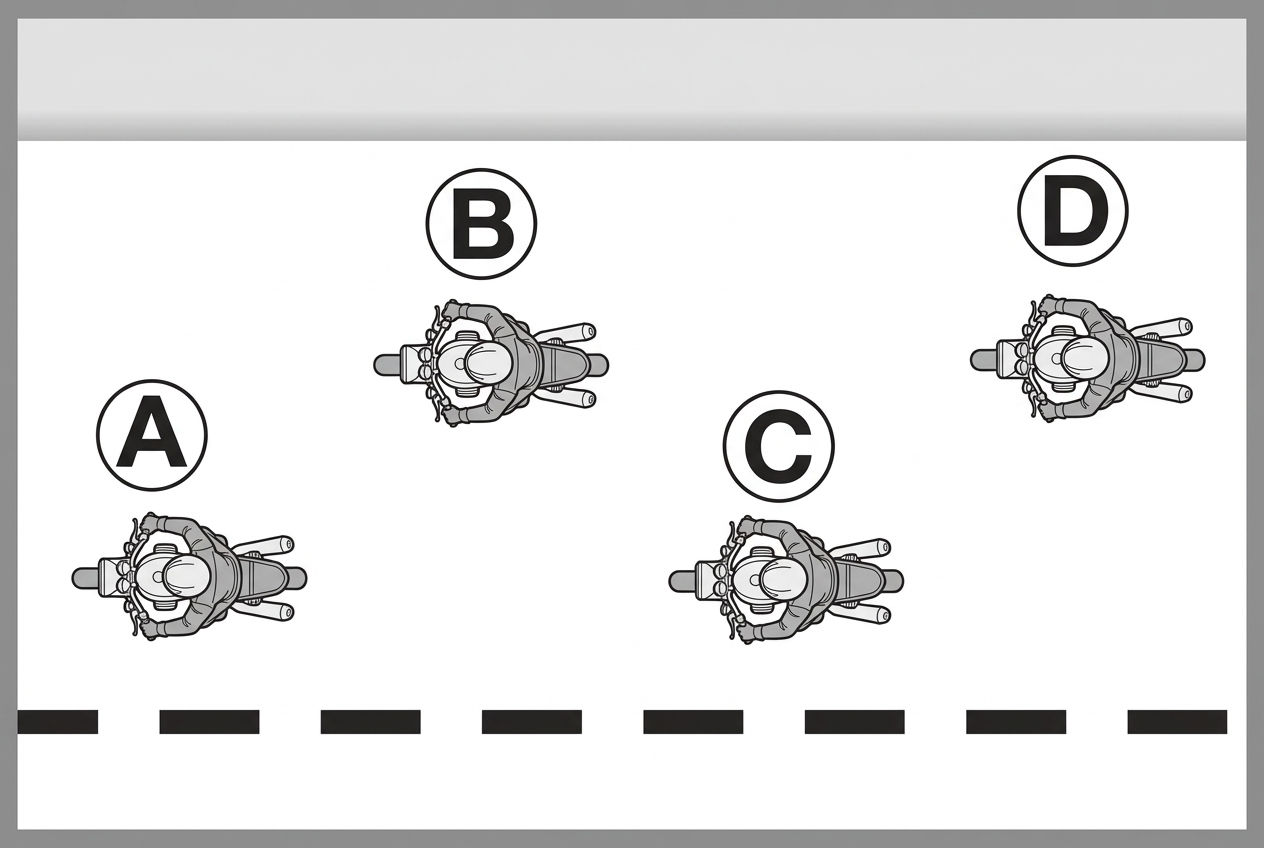
\includegraphics[width=0.8\linewidth]{ q_8.jpeg }
\captionof*{figure}{ Four motorcycles (labeled A, B, C, D) riding in a staggered formation along a multi-lane road, where A is a leader in left portion, B after leader in right portion, C is third, in left portion and behind the leader. }

\begin{itemize}[nosep,leftmargin=2em]
\item [A.] Four seconds.
\item [B.] One car length.
\item [C.] One second.
\item [D.] Two seconds.

\end{itemize}
\end{minipage}


\begin{minipage}{\linewidth}
\vspace{1em}\noindent\textbf{9. Riders in a staggered formation will be passing a car. After the lead rider passes, he/she should:}

\begin{itemize}[nosep,leftmargin=2em]
\item [A.] Return to the right portion of the lane.
\item [B.] Return to the center portion of the lane.
\item [C.] Return to the left portion of the lane.
\item [D.] Signal the others to follow.

\end{itemize}
\end{minipage}


\begin{minipage}{\linewidth}
\vspace{1em}\noindent\textbf{10. Alcohol enters the bloodstream and quickly reaches the brain. What is affected first?}

\begin{itemize}[nosep,leftmargin=2em]
\item [A.] Judgment.
\item [B.] Speech.
\item [C.] Balance.
\item [D.] Vision.

\end{itemize}
\end{minipage}


\begin{minipage}{\linewidth}
\vspace{1em}\noindent\textbf{11. Alcohol first affects your:}

\begin{itemize}[nosep,leftmargin=2em]
\item [A.] Vision.
\item [B.] Speech.
\item [C.] Judgment.
\item [D.] Balance.

\end{itemize}
\end{minipage}


\begin{minipage}{\linewidth}
\vspace{1em}\noindent\textbf{12. Approximately half of all motorcycle crash fatalities are caused by:}

\begin{itemize}[nosep,leftmargin=2em]
\item [A.] Road conditions.
\item [B.] The rider's helmet.
\item [C.] Alcohol Impairment.
\item [D.] Mechanical Failure.

\end{itemize}
\end{minipage}


\begin{minipage}{\linewidth}
\vspace{1em}\noindent\textbf{13. If you don't control your drinking:}

\begin{itemize}[nosep,leftmargin=2em]
\item [A.] Ride slower.
\item [B.] Allow at least an hour for each drink before riding.
\item [C.] Exercise or dance to wear the drinks off.
\item [D.] Drink hot coffee to be alert

\end{itemize}
\end{minipage}


\begin{minipage}{\linewidth}
\vspace{1em}\noindent\textbf{14. Studies show that almost half of all riders killed in motorcycle crashes:}

\begin{itemize}[nosep,leftmargin=2em]
\item [A.] Had poor eyesight.
\item [B.] Had been drinking.
\item [C.] Were speeding.
\item [D.] Were unskilled.

\end{itemize}
\end{minipage}


\begin{minipage}{\linewidth}
\vspace{1em}\noindent\textbf{15. The ability to think clearly and ride safely is affected by as little as:}

\begin{itemize}[nosep,leftmargin=2em]
\item [A.] 1 drink.
\item [B.] 6 drinks.
\item [C.] 3 drinks.
\item [D.] 2 drinks.

\end{itemize}
\end{minipage}


\begin{minipage}{\linewidth}
\vspace{1em}\noindent\textbf{16. If you drink 4 typical drinks, what is the least amount of alcohol remaining in your body after 2 hrs?}

\begin{itemize}[nosep,leftmargin=2em]
\item [A.] 2 drinks.
\item [B.] 3 drinks.
\item [C.] 1 drink.
\item [D.] 4 drinks.

\end{itemize}
\end{minipage}


\begin{minipage}{\linewidth}
\vspace{1em}\noindent\textbf{17. For greatest safety, your helmet should:}

\begin{itemize}[nosep,leftmargin=2em]
\item [A.] Fit tightly at the base; loosely at the top.
\item [B.] Fit loosely all the way around.
\item [C.] Fit snugly all the way around.
\item [D.] Be worn only on long rides.

\end{itemize}
\end{minipage}


\begin{minipage}{\linewidth}
\vspace{1em}\noindent\textbf{18. The single most important thing you can do to improve your chances of surviving a crash is to:}

\begin{itemize}[nosep,leftmargin=2em]
\item [A.] Lay the motorcycle down before hitting an obstacle.
\item [B.] Wear a securely fastened helmet.
\item [C.] Be familiar with the motorcycle.
\item [D.] Ride in the center portion of the lane.

\end{itemize}
\end{minipage}


\begin{minipage}{\linewidth}
\vspace{1em}\noindent\textbf{19. Wearing a helmet can reduce the chance of a fatal head injury in:}

\begin{itemize}[nosep,leftmargin=2em]
\item [A.] Low-speed crash only.
\item [B.] Single-vehicle crashes only.
\item [C.] Any crash, regardless of speed.
\item [D.] High-speed crash only.

\end{itemize}
\end{minipage}


\begin{minipage}{\linewidth}
\vspace{1em}\noindent\textbf{20. Wearing a helmet will:}

\begin{itemize}[nosep,leftmargin=2em]
\item [A.] Reduce your chances of neck and head injuries.
\item [B.] Increase your chances of a neck injury.
\item [C.] Reduce your vision by two-thirds.
\item [D.] Neither reduce nor increase your chances of a head injury.

\end{itemize}
\end{minipage}


\begin{minipage}{\linewidth}
\vspace{1em}\noindent\textbf{21. Of the following, which one gives the most eye and face protection while riding?}

\begin{itemize}[nosep,leftmargin=2em]
\item [A.] Goggles.
\item [B.] A windshield.
\item [C.] A faceshield.
\item [D.] Sunglasses.

\end{itemize}
\end{minipage}


\begin{minipage}{\linewidth}
\vspace{1em}\noindent\textbf{22. While riding an unfamiliar motorcycle:}

\begin{itemize}[nosep,leftmargin=2em]
\item [A.] Do not shift above third gear.
\item [B.] Stay in the right portion of the lane.
\item [C.] Have the owner ride with you.
\item [D.] Allow extra room for stopping.

\end{itemize}
\end{minipage}


\begin{minipage}{\linewidth}
\vspace{1em}\noindent\textbf{23. The engine cut-off switch is usually located:}

\begin{itemize}[nosep,leftmargin=2em]
\item [A.] Near the clutch.
\item [B.] On the left handlebar.
\item [C.] Near the right hand grip.
\item [D.] On the top of the gas tank.

\end{itemize}
\end{minipage}


\begin{minipage}{\linewidth}
\vspace{1em}\noindent\textbf{24. With a properly adjusted mirror you can see:}

\begin{itemize}[nosep,leftmargin=2em]
\item [A.] The lane beside you.
\item [B.] The lane behind you.
\item [C.] Part of the lane beside you and behind you.
\item [D.] Everything behind and to the side.

\end{itemize}
\end{minipage}


\begin{minipage}{\linewidth}
\vspace{1em}\noindent\textbf{25. When slowing for a normal stop:}

\begin{itemize}[nosep,leftmargin=2em]
\item [A.] Use only the rear brake.
\item [B.] Use less throttle and the front brake only.
\item [C.] Shift down through the gears as you slow.
\item [D.] Pull in the clutch and coast.

\end{itemize}
\end{minipage}


\begin{minipage}{\linewidth}
\vspace{1em}\noindent\textbf{26. When turning, you should:}

\begin{itemize}[nosep,leftmargin=2em]
\item [A.] Watch the center line.
\item [B.] Look straight ahead.
\item [C.] Look at the guard rail.
\item [D.] Look through the turn.

\end{itemize}
\end{minipage}


\begin{minipage}{\linewidth}
\vspace{1em}\noindent\textbf{27. Which one of the following statements is correct:}

\begin{itemize}[nosep,leftmargin=2em]
\item [A.] Press left, lean left, go right.
\item [B.] Press left, lean left, go left.
\item [C.] Press left, lean right, go right.
\item [D.] Press right, lean right, go left.

\end{itemize}
\end{minipage}


\begin{minipage}{\linewidth}
\vspace{1em}\noindent\textbf{28. While in a turn, it is best to:}

\begin{itemize}[nosep,leftmargin=2em]
\item [A.] Maintain a steady speed or gradually accelerate.
\item [B.] Slow down.
\item [C.] Use your brakes.
\item [D.] Accelerate and look straight ahead.

\end{itemize}
\end{minipage}


\begin{minipage}{\linewidth}
\vspace{1em}\noindent\textbf{29. If you need to slow down while turning:}

\begin{itemize}[nosep,leftmargin=2em]
\item [A.] Apply the rear brake, and lean farther into the turn.
\item [B.] Never apply the brakes.
\item [C.] Use caution, apply both brakes.
\item [D.] Apply the rear brake only.

\end{itemize}
\end{minipage}


\begin{minipage}{\linewidth}
\vspace{1em}\noindent\textbf{30. To make a normal stop, use:}

\begin{itemize}[nosep,leftmargin=2em]
\item [A.] The rear brake first.
\item [B.] Both brakes, and downshift.
\item [C.] The front brake and downshift.
\item [D.] The rear brake only.

\end{itemize}
\end{minipage}


\begin{minipage}{\linewidth}
\vspace{1em}\noindent\textbf{31. Your motorcycle has two brakes. Use both brakes:}

\begin{itemize}[nosep,leftmargin=2em]
\item [A.] Only for emergency stops.
\item [B.] While swerving.
\item [C.] Every time you slow or stop.
\item [D.] Only for normal stops.

\end{itemize}
\end{minipage}


\begin{minipage}{\linewidth}
\vspace{1em}\noindent\textbf{32. In a normal turn:}

\begin{itemize}[nosep,leftmargin=2em]
\item [A.] Lean your motorcycle more than your body.
\item [B.] Lean your motorcycle and your body at the same angle.
\item [C.] Do not lean.
\item [D.] Lean your body more than your motorcycle.

\end{itemize}
\end{minipage}


\begin{minipage}{\linewidth}
\vspace{1em}\noindent\textbf{33. In slow tight turns:}

\begin{itemize}[nosep,leftmargin=2em]
\item [A.] Lean the motorcycle only, and keep your body straight.
\item [B.] Lean your body more than the motorcycle.
\item [C.] Lean with the motorcycle.
\item [D.] Do not lean.

\end{itemize}
\end{minipage}


\begin{minipage}{\linewidth}
\vspace{1em}\noindent\textbf{34. To reduce speed before turning:}

\begin{itemize}[nosep,leftmargin=2em]
\item [A.] Shift to neutral.
\item [B.] Pull in the clutch and use both brakes.
\item [C.] Apply the rear brake only.
\item [D.] Close the throttle and apply both brakes.

\end{itemize}
\end{minipage}


\begin{minipage}{\linewidth}
\vspace{1em}\noindent\textbf{35. When turning, it is important to:}

\begin{itemize}[nosep,leftmargin=2em]
\item [A.] Look straight ahead.
\item [B.] Slow after starting into the turn.
\item [C.] Reduce speed coming out of the turn.
\item [D.] Look through the turn to where you want to go.

\end{itemize}
\end{minipage}


\begin{minipage}{\linewidth}
\vspace{1em}\noindent\textbf{36. It is important to search the road for escape routes:}

\begin{itemize}[nosep,leftmargin=2em]
\item [A.] Through alleyways.
\item [B.] At intersections.
\item [C.] When riding a borrowed motorcycle.
\item [D.] On curves.

\end{itemize}
\end{minipage}


\begin{minipage}{\linewidth}
\vspace{1em}\noindent\textbf{37. To make good judgments in traffic, you need to first:}

\begin{itemize}[nosep,leftmargin=2em]
\item [A.] Be able to swerve.
\item [B.] Search ahead.
\item [C.] Watch for pedestrians.
\item [D.] Know how to stop quickly.

\end{itemize}
\end{minipage}


\begin{minipage}{\linewidth}
\vspace{1em}\noindent\textbf{38. The car driver is signaling for a left turn. The rider should:}

\vspace{1ex}
\centering
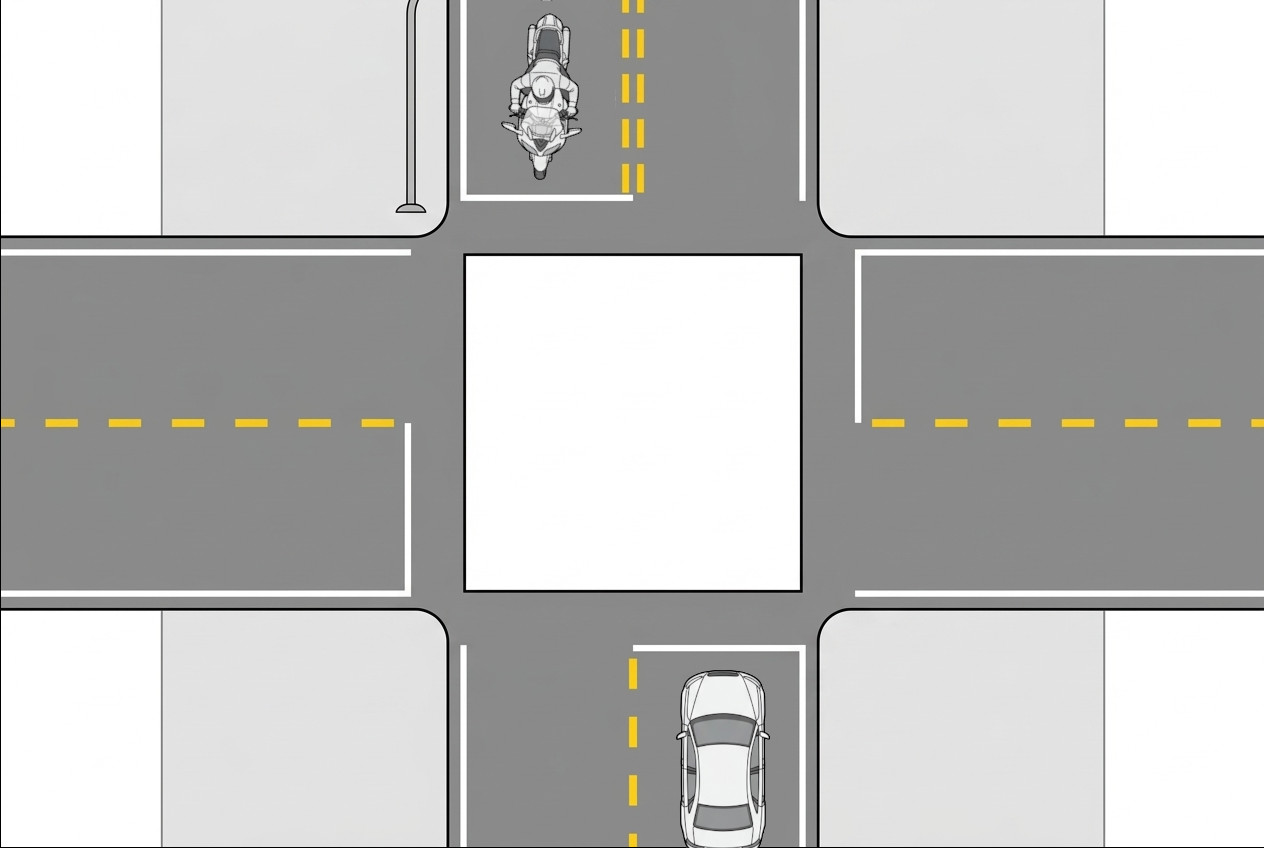
\includegraphics[width=0.8\linewidth]{ q_38.jpeg }
\captionof*{figure}{ A scene at an intersection where a motorcycle and a car meet at the intersection. The motorcycle is driving straight ahead, while the car is turning in front of motorcycle. The motorcycle has the right-of-way. }

\begin{itemize}[nosep,leftmargin=2em]
\item [A.] Hold speed and center lane position.
\item [B.] Slow and move away from approaching vehicles.
\item [C.] Increase speed and move left.
\item [D.] Increase speed and stay in the center of the lane.

\end{itemize}
\end{minipage}


\begin{minipage}{\linewidth}
\vspace{1em}\noindent\textbf{39. You should make a special point of checking traffic to the rear:}

\begin{itemize}[nosep,leftmargin=2em]
\item [A.] Before starting into a curve.
\item [B.] When you approach an intersection.
\item [C.] When carrying a passenger.
\item [D.] Before slowing.

\end{itemize}
\end{minipage}


\begin{minipage}{\linewidth}
\vspace{1em}\noindent\textbf{40. When preparing to pass, it is usually better to:}

\begin{itemize}[nosep,leftmargin=2em]
\item [A.] Signal, check your left mirror,  look left.
\item [B.] Signal, move into left lane, accelerate.
\item [C.] Signal, check your left mirror.
\item [D.] Signal, Check your left mirror, speed up.

\end{itemize}
\end{minipage}


\begin{minipage}{\linewidth}
\vspace{1em}\noindent\textbf{41. Riding in the center lane position:}

\begin{itemize}[nosep,leftmargin=2em]
\item [A.] Keeps others from seeing you.
\item [B.] Is safest place when approaching intersections.
\item [C.] Keeps others from sharing your lane.
\item [D.] Should be avoided if possible.

\end{itemize}
\end{minipage}


\begin{minipage}{\linewidth}
\vspace{1em}\noindent\textbf{42. To discourage other drivers from sharing your lane, it is usually best to:}

\begin{itemize}[nosep,leftmargin=2em]
\item [A.] Ride in the left portion of your lane.
\item [B.] Ride in the center portion of your lane.
\item [C.] Ride next to another vehicle.
\item [D.] Ride in the right portion of your lane.

\end{itemize}
\end{minipage}


\begin{minipage}{\linewidth}
\vspace{1em}\noindent\textbf{43. Keeping a cushion of space around your motorcycle:}

\begin{itemize}[nosep,leftmargin=2em]
\item [A.] Is only necessary for beginning motorcyclists.
\item [B.] Allows you time and space to react.
\item [C.] Allows you to weave through traffic when you need to.
\item [D.] Makes you more vulnerable.

\end{itemize}
\end{minipage}


\begin{minipage}{\linewidth}
\vspace{1em}\noindent\textbf{44. To spot approaching traffic and maintain a space cushion in the illustration above:}

\vspace{1ex}
\centering
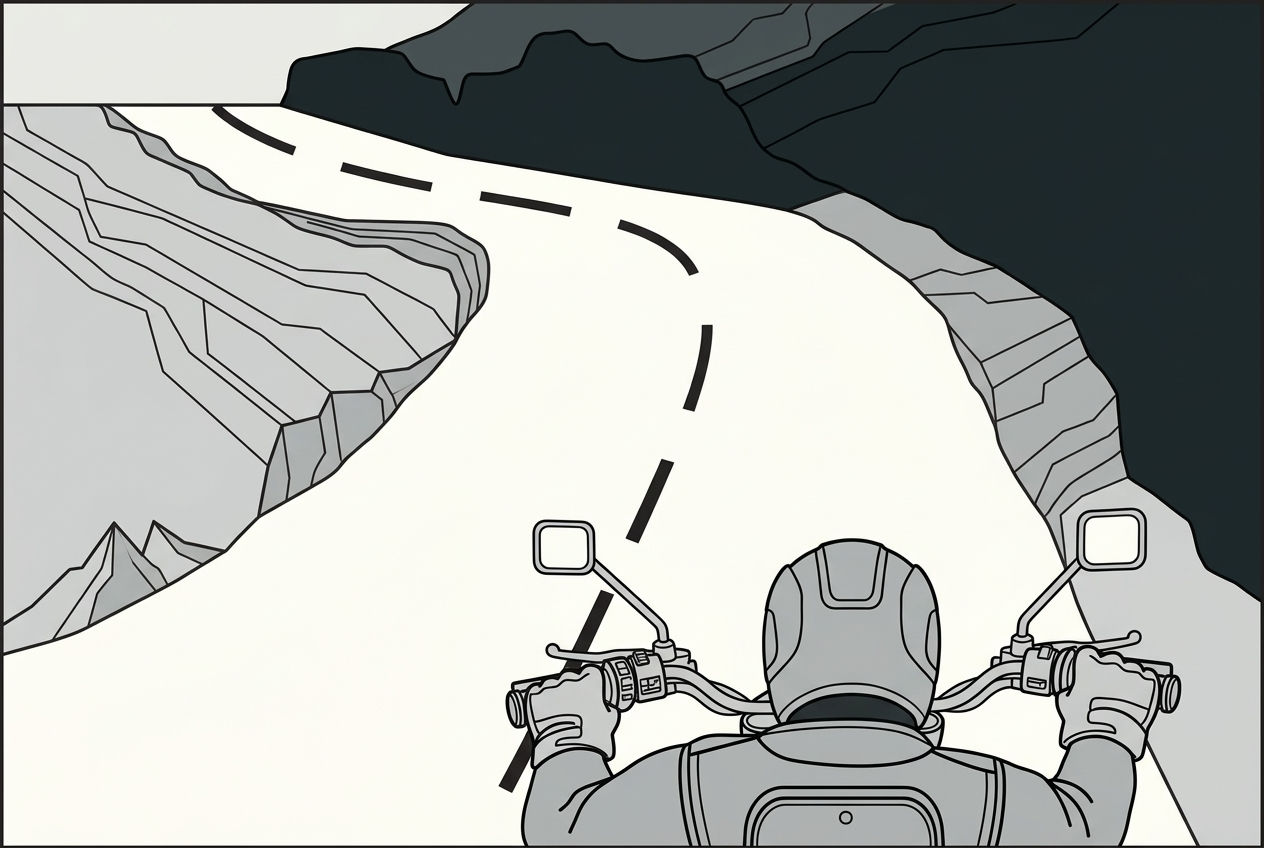
\includegraphics[width=0.8\linewidth]{ q_44.jpeg }
\captionof*{figure}{ Looking ahead at a winding road curve }

\begin{itemize}[nosep,leftmargin=2em]
\item [A.] Ride in the center of the lane.
\item [B.] Move right and lean away from the turn.
\item [C.] Do not lean.
\item [D.] Ride in the left portion of the lane.

\end{itemize}
\end{minipage}


\begin{minipage}{\linewidth}
\vspace{1em}\noindent\textbf{45. You plan to make a right turn after stopping at an intersection. Usually it is best to:}

\begin{itemize}[nosep,leftmargin=2em]
\item [A.] Let the traffic coming from behind pass around you.
\item [B.] Turn from the center portion of the lane.
\item [C.] Turn from the right portion of the lane.
\item [D.] Turn from the left portion of the lane.

\end{itemize}
\end{minipage}


\begin{minipage}{\linewidth}
\vspace{1em}\noindent\textbf{46. Following close to vehicles in front of you:}

\begin{itemize}[nosep,leftmargin=2em]
\item [A.] Helps you see hazards in the road.
\item [B.] Is safer at night.
\item [C.] Protects you in heavy traffic.
\item [D.] Is a factor in crashes caused by motorcyclists.

\end{itemize}
\end{minipage}


\begin{minipage}{\linewidth}
\vspace{1em}\noindent\textbf{47. When following a car, you should try to:}

\begin{itemize}[nosep,leftmargin=2em]
\item [A.] Ride where the driver can see you in the rear-view mirror.
\item [B.] Ride next to another car to be more visible.
\item [C.] Ride in the left side of the lane.
\item [D.] Ride in the right side of the lane.

\end{itemize}
\end{minipage}


\begin{minipage}{\linewidth}
\vspace{1em}\noindent\textbf{48. At intersections, the most common cause of motorcycle/car crashes is:}

\begin{itemize}[nosep,leftmargin=2em]
\item [A.] Drivers entering a rider's right of way.
\item [B.] Riders not seeing drivers enter from side streets.
\item [C.] Drivers tailgating riders.
\item [D.] Riders not yielding to oncoming traffic.

\end{itemize}
\end{minipage}


\begin{minipage}{\linewidth}
\vspace{1em}\noindent\textbf{49. Car/Motorcycle crashes are most common:}

\begin{itemize}[nosep,leftmargin=2em]
\item [A.] At intersections.
\item [B.] At night.
\item [C.] When the rider is speeding.
\item [D.] On freeways.

\end{itemize}
\end{minipage}


\begin{minipage}{\linewidth}
\vspace{1em}\noindent\textbf{50. Making eye contact with a driver at an intersection:}

\begin{itemize}[nosep,leftmargin=2em]
\item [A.] Is a sure sign that the driver will probably yield.
\item [B.] Is important if the driver is pulling out from a side street.
\item [C.] Does not mean that the driver sees you.
\item [D.] Confuses them.

\end{itemize}
\end{minipage}


\begin{minipage}{\linewidth}
\vspace{1em}\noindent\textbf{51. The greatest danger for a rider when passing parked cars is:}

\begin{itemize}[nosep,leftmargin=2em]
\item [A.] A car backing into a parking space.
\item [B.] A car pulling out.
\item [C.] A car door being opened.
\item [D.] Someone stepping from between cars.

\end{itemize}
\end{minipage}


\begin{minipage}{\linewidth}
\vspace{1em}\noindent\textbf{52. In this picture, the light most likely to make the motorcycle noticeable to the car driver is the:}

\vspace{1ex}
\centering
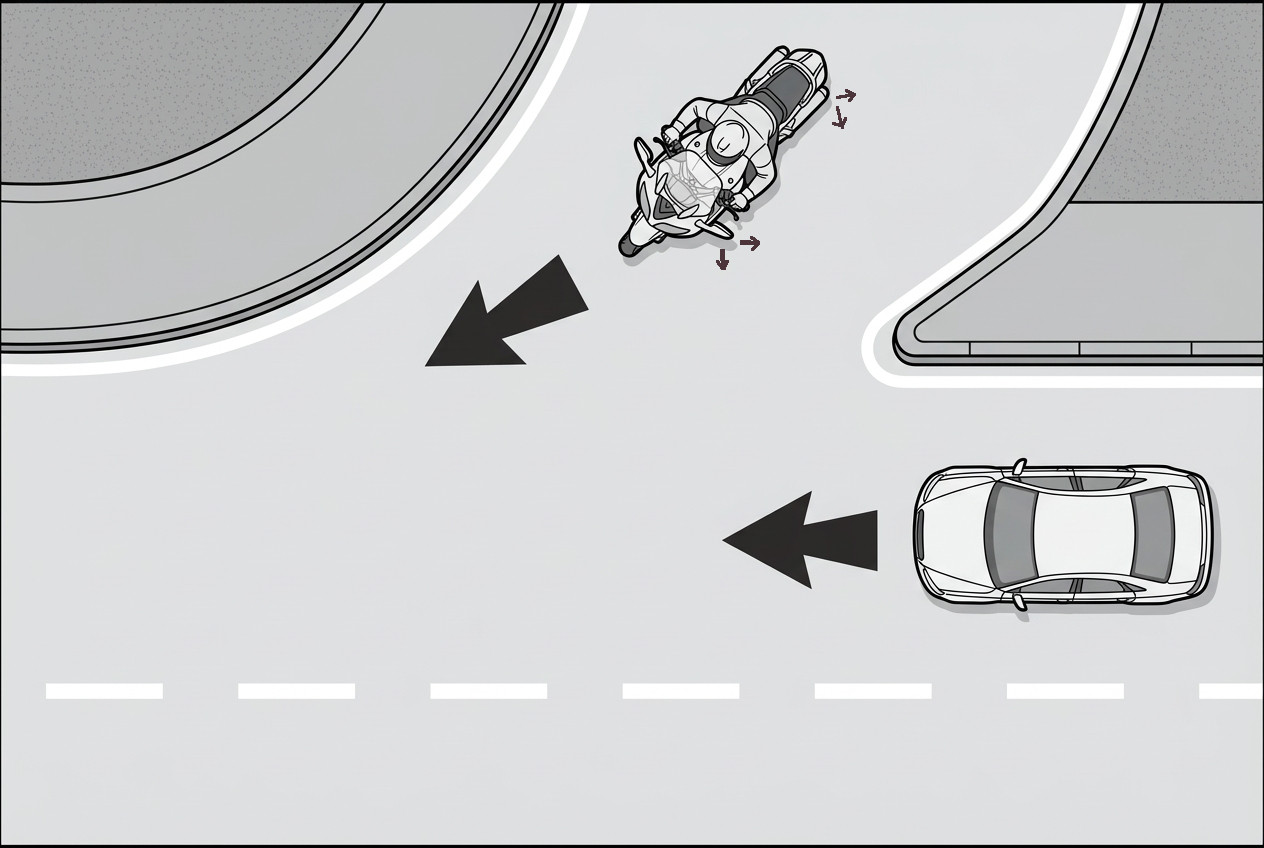
\includegraphics[width=0.8\linewidth]{ q_52.jpeg }
\captionof*{figure}{ Rider merges highway when there is a car in right lane on the highway }

\begin{itemize}[nosep,leftmargin=2em]
\item [A.] Brake light.
\item [B.] Taillight.
\item [C.] Headlight.
\item [D.] Turn signal.

\end{itemize}
\end{minipage}


\begin{minipage}{\linewidth}
\vspace{1em}\noindent\textbf{53. When riding in traffic at night, the best way to locate bumps in the road is to:}

\begin{itemize}[nosep,leftmargin=2em]
\item [A.] Look over the cars ahead.
\item [B.] Put your headlights on high beam.
\item [C.] Read the road signs.
\item [D.] Watch the taillights of the car ahead.

\end{itemize}
\end{minipage}


\begin{minipage}{\linewidth}
\vspace{1em}\noindent\textbf{54. The best way to help others see your motorcycle is to:}

\begin{itemize}[nosep,leftmargin=2em]
\item [A.] Ride in the left portion of the lane.
\item [B.] Wear a white helmet.
\item [C.] Stay in the center portion of the lane.
\item [D.] Ride with your headlight turned on.

\end{itemize}
\end{minipage}


\begin{minipage}{\linewidth}
\vspace{1em}\noindent\textbf{55. Not turning off a turn signal is most likely to:}

\begin{itemize}[nosep,leftmargin=2em]
\item [A.] Encourage other drivers to pull into your path.
\item [B.] Keeps others from noticing your brake light.
\item [C.] Reduces your chances of a crash because other drivers stay clear.
\item [D.] Encourage others to follow you too closely.

\end{itemize}
\end{minipage}


\begin{minipage}{\linewidth}
\vspace{1em}\noindent\textbf{56. Make a special point to use your mirrors:}

\begin{itemize}[nosep,leftmargin=2em]
\item [A.] On long trips.
\item [B.] When riding through an intersection.
\item [C.] When following a vehicle.
\item [D.] Before slowing or stopping.

\end{itemize}
\end{minipage}


\begin{minipage}{\linewidth}
\vspace{1em}\noindent\textbf{57. Before changing lanes to the left:}

\begin{itemize}[nosep,leftmargin=2em]
\item [A.] Check your left mirror; and look to the left.
\item [B.] Check the right mirror, then the left mirror.
\item [C.] Check the left mirror, then the right mirror.
\item [D.] Use your horn and speed up.

\end{itemize}
\end{minipage}


\begin{minipage}{\linewidth}
\vspace{1em}\noindent\textbf{58. The best gear to wear to be seen at night is:}

\begin{itemize}[nosep,leftmargin=2em]
\item [A.] Fluorescent clothing.
\item [B.] A white helmet.
\item [C.] Reflective clothing.
\item [D.] A red jacket.

\end{itemize}
\end{minipage}


\begin{minipage}{\linewidth}
\vspace{1em}\noindent\textbf{59. To see better when following a car at night:}

\begin{itemize}[nosep,leftmargin=2em]
\item [A.] Increase your following distance and use your low beam.
\item [B.] Use the headlights of the vehicle ahead.
\item [C.] Pass when safe and use your high beam.
\item [D.] Drop far back and use your high beam.

\end{itemize}
\end{minipage}


\begin{minipage}{\linewidth}
\vspace{1em}\noindent\textbf{60. When riding at night:}

\begin{itemize}[nosep,leftmargin=2em]
\item [A.] Always ride in the center lane.
\item [B.] Ride with flashers on.
\item [C.] Wear reflective clothing.
\item [D.] Follow closer to the vehicle ahead for safety.

\end{itemize}
\end{minipage}


\begin{minipage}{\linewidth}
\vspace{1em}\noindent\textbf{61. If you lock the front tire when stopping:}

\begin{itemize}[nosep,leftmargin=2em]
\item [A.] Release the rear brake.
\item [B.] Keep the front brake locked until fully stopped.
\item [C.] Keep both brakes locked.
\item [D.] Release and reapply the front brake.

\end{itemize}
\end{minipage}


\begin{minipage}{\linewidth}
\vspace{1em}\noindent\textbf{62. In the picture above, the rear wheel locks while trying to stop quickly. It is usually best to:}

\vspace{1ex}
\centering
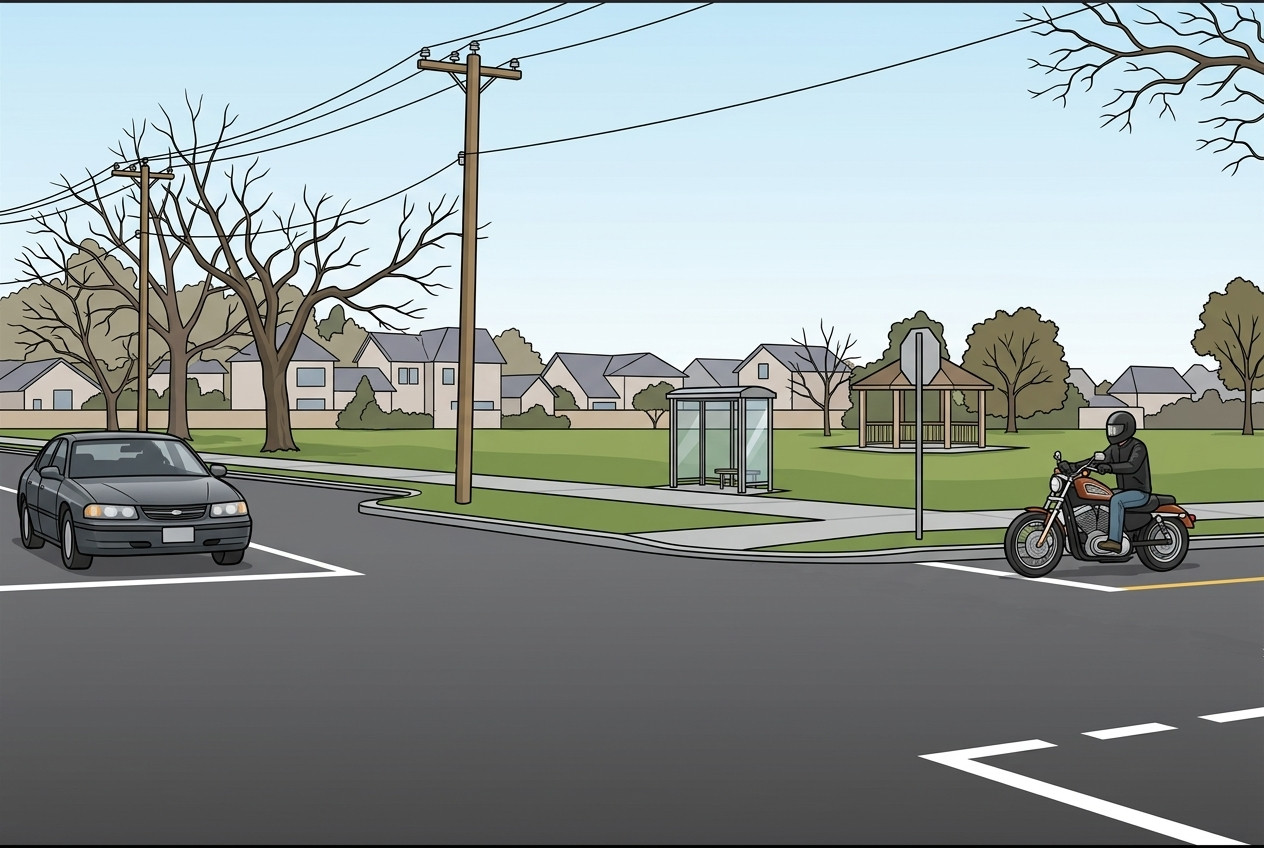
\includegraphics[width=0.8\linewidth]{ q_62.jpeg }
\captionof*{figure}{ A street intersection in a suburban neighborhood with a car on the left and a motorcycle on the right aproaching the eachother. }

\begin{itemize}[nosep,leftmargin=2em]
\item [A.] Maintain position and release the rear brake.
\item [B.] Lean the motorcycle and release the rear brake.
\item [C.] Release front brake and keep rear brake locked.
\item [D.] Keep the rear wheel locked until stopped.

\end{itemize}
\end{minipage}


\begin{minipage}{\linewidth}
\vspace{1em}\noindent\textbf{63. When swerving, it is important to:}

\begin{itemize}[nosep,leftmargin=2em]
\item [A.] Always brake before swerving.
\item [B.] Separate braking from swerving.
\item [C.] Always brake after swerving.
\item [D.] Swerve in the direction the hazard is traveling.

\end{itemize}
\end{minipage}


\begin{minipage}{\linewidth}
\vspace{1em}\noindent\textbf{64. To ride over metal bridge gratings:}

\begin{itemize}[nosep,leftmargin=2em]
\item [A.] Ride straight across.
\item [B.] Weave (zig-zag) across.
\item [C.] Cross at a sharp angle without changing lanes.
\item [D.] Speed up.

\end{itemize}
\end{minipage}


\begin{minipage}{\linewidth}
\vspace{1em}\noindent\textbf{65. To ride over an object on the road:}

\begin{itemize}[nosep,leftmargin=2em]
\item [A.] Stay seated until you have crossed it.
\item [B.] Rise slightly off the seat.
\item [C.] Edge across it.
\item [D.] Grip the gas tank with your knees.

\end{itemize}
\end{minipage}


\begin{minipage}{\linewidth}
\vspace{1em}\noindent\textbf{66. When riding over an obstacle, it is usually best to:}

\begin{itemize}[nosep,leftmargin=2em]
\item [A.] Keep a normal seat position.
\item [B.] Rise slightly off the seat.
\item [C.] Grip the gas tank with your knees.
\item [D.] Lean forward as much as possible.

\end{itemize}
\end{minipage}


\begin{minipage}{\linewidth}
\vspace{1em}\noindent\textbf{67. On a paved, two-lane road, sand and gravel are most likely to collect:}

\begin{itemize}[nosep,leftmargin=2em]
\item [A.] In the left wheel track.
\item [B.] Near the center of the road.
\item [C.] Near the sides of the road.
\item [D.] In the center of the lane.

\end{itemize}
\end{minipage}


\begin{minipage}{\linewidth}
\vspace{1em}\noindent\textbf{68. On a wet road, it will usually be most slippery:}

\begin{itemize}[nosep,leftmargin=2em]
\item [A.] On loose gravel.
\item [B.] In the left wheel track.
\item [C.] In the right wheel track.
\item [D.] In the center portion of the lane.

\end{itemize}
\end{minipage}


\begin{minipage}{\linewidth}
\vspace{1em}\noindent\textbf{69. To handle a slippery surface, it is best to:}

\begin{itemize}[nosep,leftmargin=2em]
\item [A.] Use the rear brake lightly while crossing.
\item [B.] Slow down before reaching it.
\item [C.] Gradually accelerate.
\item [D.] Downshift when you reach it.

\end{itemize}
\end{minipage}


\begin{minipage}{\linewidth}
\vspace{1em}\noindent\textbf{70. To stop on wet pavement:}

\begin{itemize}[nosep,leftmargin=2em]
\item [A.] Apply the front brake only if the wheel begins to slide.
\item [B.] Coast to a stop.
\item [C.] Apply the rear brake only.
\item [D.] Apply the front and rear brakes together.

\end{itemize}
\end{minipage}


\begin{minipage}{\linewidth}
\vspace{1em}\noindent\textbf{71. When riding where sand and gravel have collected on paved roads, you should:}

\begin{itemize}[nosep,leftmargin=2em]
\item [A.] Downshift and use more throttle.
\item [B.] Pull-in the clutch.
\item [C.] Only use the rear brake to slow down.
\item [D.] Avoid sudden changes in speed or direction.

\end{itemize}
\end{minipage}


\begin{minipage}{\linewidth}
\vspace{1em}\noindent\textbf{72. If the rear tire goes flat:}

\begin{itemize}[nosep,leftmargin=2em]
\item [A.] You will not be able to maintain control.
\item [B.] You will lose power to the rear wheel.
\item [C.] The back of the motorcycle will jerk from side to side.
\item [D.] The steering will feel heavy.

\end{itemize}
\end{minipage}


\begin{minipage}{\linewidth}
\vspace{1em}\noindent\textbf{73. If you have a flat tire while riding, hold the handle grips firmly and:}

\begin{itemize}[nosep,leftmargin=2em]
\item [A.] Gently apply both brakes.
\item [B.] Use the brake of the good tire or avoid braking.
\item [C.] Continue to the nearest repair facility.
\item [D.] Use only the brake that controls the flat tire.

\end{itemize}
\end{minipage}


\begin{minipage}{\linewidth}
\vspace{1em}\noindent\textbf{74. When the front tire goes flat while riding:}

\begin{itemize}[nosep,leftmargin=2em]
\item [A.] Apply the front brake.
\item [B.] You will not be able to control the motorcycle.
\item [C.] Apply rear brake and steer to the edge of the road.
\item [D.] Steer to the right and apply both brakes.

\end{itemize}
\end{minipage}


\begin{minipage}{\linewidth}
\vspace{1em}\noindent\textbf{75. When the front tire goes flat:}

\begin{itemize}[nosep,leftmargin=2em]
\item [A.] The steering will feel heavy.
\item [B.] It has no effect on handling.
\item [C.] The back of the motorcycle will jerk from side to side.
\item [D.] You will lose power to the brakes.

\end{itemize}
\end{minipage}


\begin{minipage}{\linewidth}
\vspace{1em}\noindent\textbf{76. If your throttle sticks:}

\begin{itemize}[nosep,leftmargin=2em]
\item [A.] Squeeze the clutch and use engine cut-off switch.
\item [B.] Shift to neutral and apply both brakes.
\item [C.] Downshift and apply both brakes.
\item [D.] Apply the front brake.

\end{itemize}
\end{minipage}


\begin{minipage}{\linewidth}
\vspace{1em}\noindent\textbf{77. In the picture above, it is usually best to:}

\vspace{1ex}
\centering
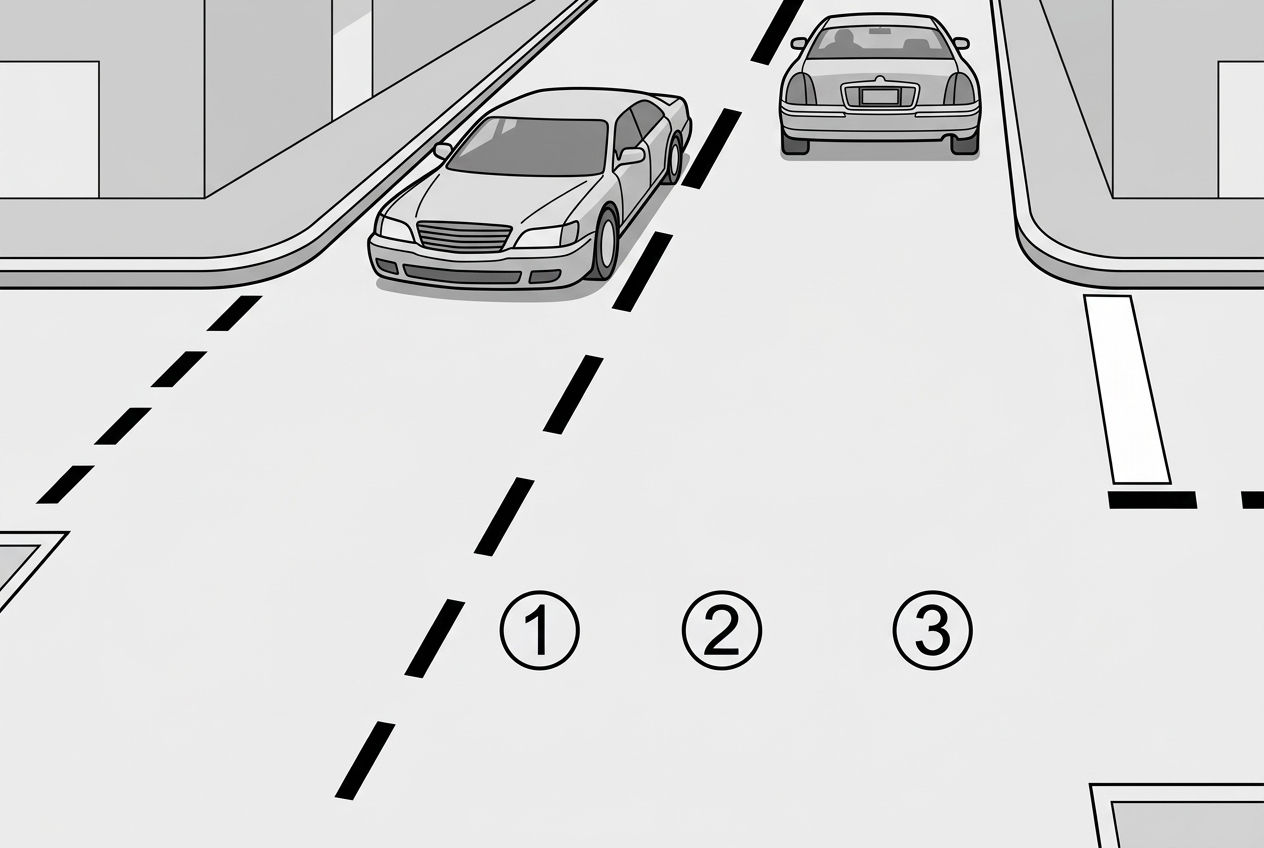
\includegraphics[width=0.8\linewidth]{ q_77.jpeg }
\captionof*{figure}{ Illustration of the lane with three numbered portions: 1 - left, 2 - center, 3 - right. }

\begin{itemize}[nosep,leftmargin=2em]
\item [A.] Speed up to get by quickly.
\item [B.] Ride in position 3.
\item [C.] Ride in position 1.
\item [D.] Ride in position 2 or 3.

\end{itemize}
\end{minipage}


\begin{minipage}{\linewidth}
\vspace{1em}\noindent\textbf{78. In this picture, A, B, and C are riding as a group. To pass, rider B should:}

\vspace{1ex}
\centering
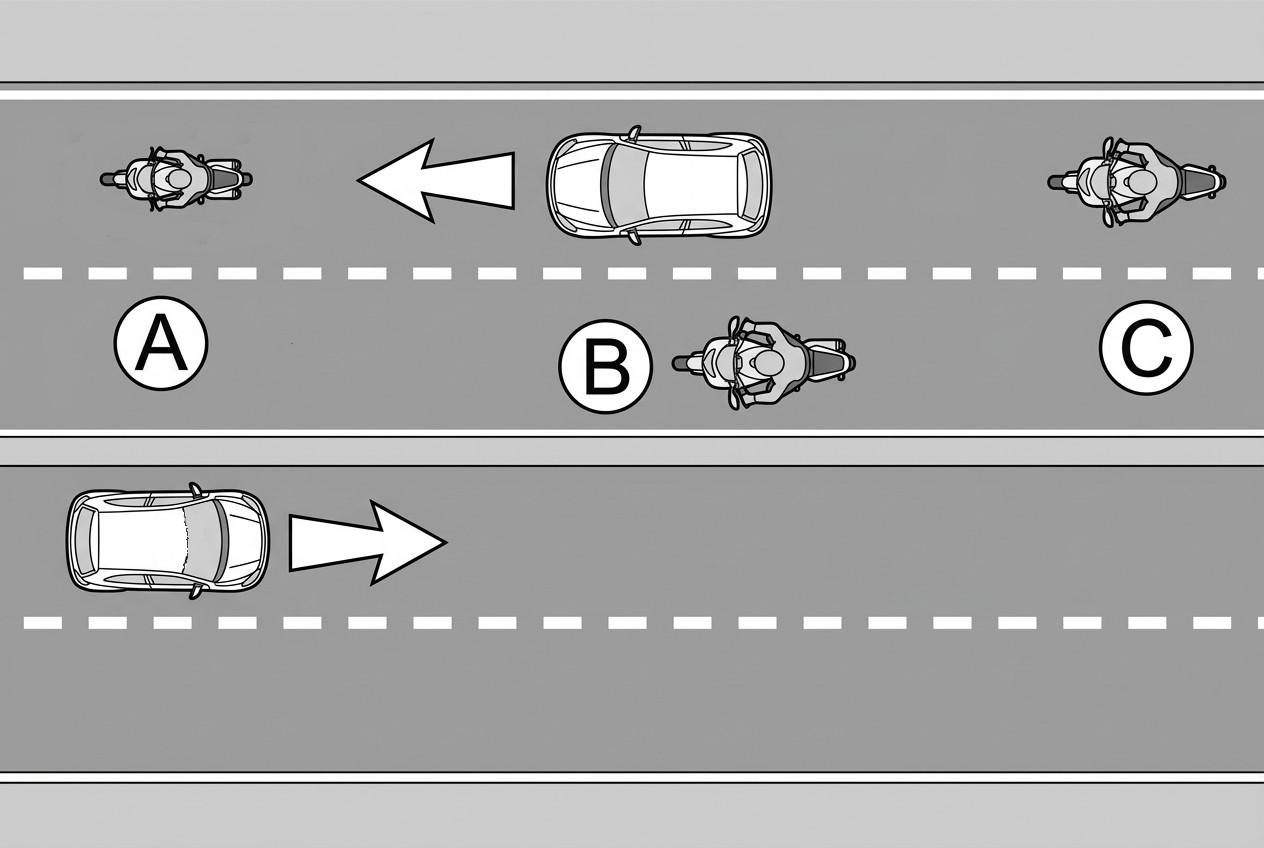
\includegraphics[width=0.8\linewidth]{ q_78.jpeg }
\captionof*{figure}{ Illustration of bike formation passing a car. A passed, B is passing, C is waiting. }

\begin{itemize}[nosep,leftmargin=2em]
\item [A.] Complete the pass in front of A.
\item [B.] Pass with C.
\item [C.] Return to the lane and ride next to A.
\item [D.] Return to the right portion of the lane behind A.

\end{itemize}
\end{minipage}


\begin{minipage}{\linewidth}
\vspace{1em}\noindent\textbf{79. To create more space in the situation pictured above, you should:}

\vspace{1ex}
\centering
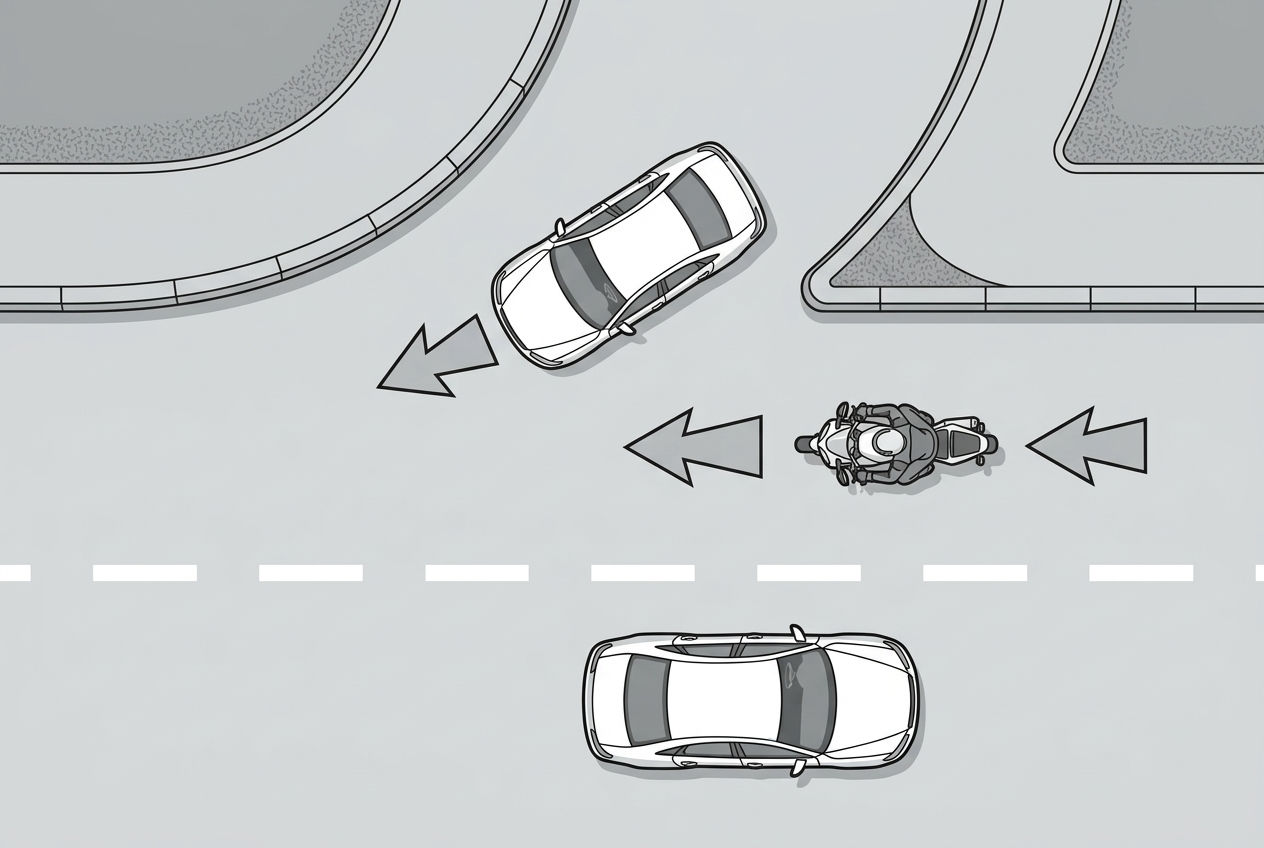
\includegraphics[width=0.8\linewidth]{ q_79.jpeg }
\captionof*{figure}{ Motorcycle driving in right lane of a highway, a car mergin to the right lane infront of  motorcycle. }

\begin{itemize}[nosep,leftmargin=2em]
\item [A.] Ride in the right portion of the lane.
\item [B.] Adjust speed and stay in the center of the lane.
\item [C.] Move to the left lane.
\item [D.] Pass the car on your left.

\end{itemize}
\end{minipage}


\begin{minipage}{\linewidth}
\vspace{1em}\noindent\textbf{80. Most motorcycle/car crashes:}

\begin{itemize}[nosep,leftmargin=2em]
\item [A.] Occur because a car driver pulls into the path of the motorcycle.
\item [B.] Result in minor injuries.
\item [C.] Occur because a motorcyclist turns left in front of a vehicle.
\item [D.] Occur because of speeding.

\end{itemize}
\end{minipage}


\begin{minipage}{\linewidth}
\vspace{1em}\noindent\textbf{81. You are preparing to move to the left lane, as pictured above. To spot cars passing beside you, it is best to:}

\vspace{1ex}
\centering
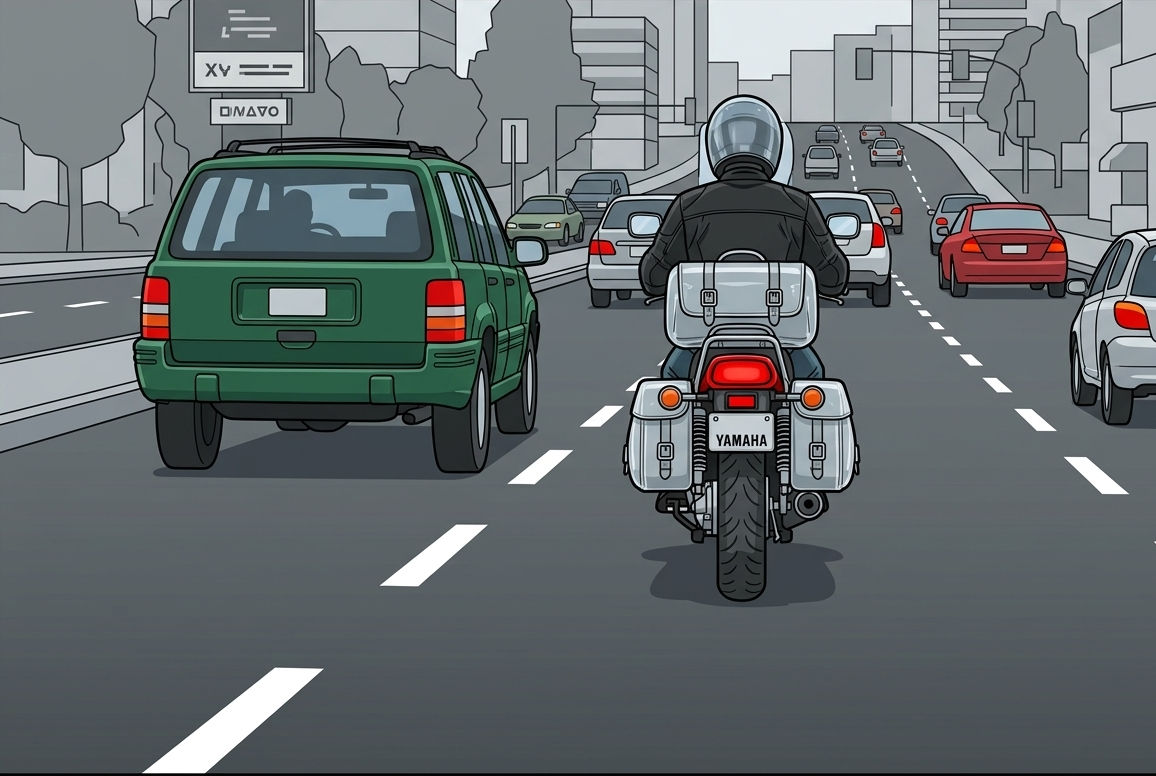
\includegraphics[width=0.8\linewidth]{ q_81.jpeg }
\captionof*{figure}{ Motorcycle in center of a middle lane. Prepearing to move to left lane. }

\begin{itemize}[nosep,leftmargin=2em]
\item [A.] Slow and look in the left mirror.
\item [B.] Look in the left mirror.
\item [C.] Speed up and look in the left mirror.
\item [D.] Turn your head to the left.

\end{itemize}
\end{minipage}


\begin{minipage}{\linewidth}
\vspace{1em}\noindent\textbf{82. To adjust for traffic and avoid debris in the curve pictured, ride:}

\vspace{1ex}
\centering

\includegraphics[width=0.8\linewidth]{ q_82.jpeg }
\captionof*{figure}{ Undivided highway curve where right side has numbered portions: 1 - left portion, 2 - center portion, 3 - right portion }

\begin{itemize}[nosep,leftmargin=2em]
\item [A.] In position 3.
\item [B.] In position 2.
\item [C.] Without leaning.
\item [D.] In position 1.

\end{itemize}
\end{minipage}


\begin{minipage}{\linewidth}
\vspace{1em}\noindent\textbf{83. To cross tracks that run parallel to your course:}

\begin{itemize}[nosep,leftmargin=2em]
\item [A.] Edge gradually across.
\item [B.] Move into the opposing lane to cross at a 90-degree angle.
\item [C.] Wait for the tracks to end.
\item [D.] Move away, then turn and cross at an angle of at least 45 degrees.

\end{itemize}
\end{minipage}


\begin{minipage}{\linewidth}
\vspace{1em}\noindent\textbf{84. In this picture, the rider in the most dangerous position is:}

\vspace{1ex}
\centering
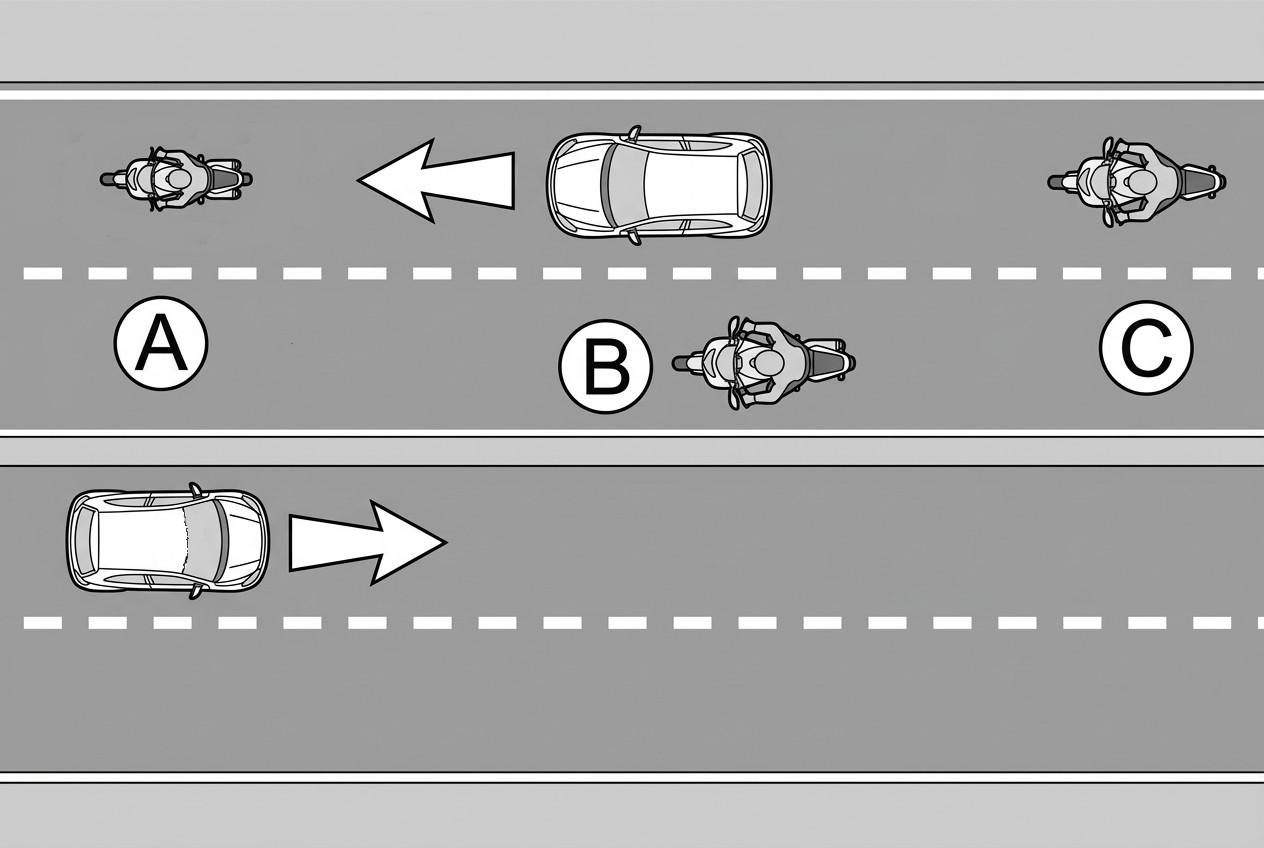
\includegraphics[width=0.8\linewidth]{ q_84.jpeg }
\captionof*{figure}{ Illustration of bike formation passing a car. A passed, B is passing, C is waiting. }

\begin{itemize}[nosep,leftmargin=2em]
\item [A.] Rider B.
\item [B.] Rider C.
\item [C.] Rider A.
\item [D.] None.

\end{itemize}
\end{minipage}


	
\end{multicols}

\clearpage
\subsection{Answer Explained EN}	
\begin{multicols}{2}
	\raggedcolumns
	\begin{minipage}{\linewidth}
\noindent\textbf{1.}  -- \textbf {(B).} When adjusting your mirrors to carry a passenger, the passenger should:  \textbf {Sit on the seat with you.} \par \textit {A passenger's weight changes the bike's attitude and your sitting position, so mirrors must be set with the passenger seated, exactly as you will ride.} \\
\end{minipage}

\begin{minipage}{\linewidth}
\noindent\textbf{2.}  -- \textbf {(C).} A passenger should:  \textbf {Hold onto the operator's waist.} \par \textit {Holding the operator's waist (or hips/belt) lets the passenger synconiusly move with the rider and lean with the bike, keeping the motorcycle stable.} \\
\end{minipage}

\begin{minipage}{\linewidth}
\noindent\textbf{3.}  -- \textbf {(A).} When the motorcycle is stopped at an intersection, a passenger should:  \textbf {Keep both feet on the foot pegs.} \par \textit {Putting feet down can unbalance the bike and risks injury, so only the operator handles the stop.} \\
\end{minipage}

\begin{minipage}{\linewidth}
\noindent\textbf{4.}  -- \textbf {(C).} When carrying a passenger:  \textbf {It will take longer to accelerate and slow down.} \par \textit {Even a small passenger is a big share of a motorcycle's total weight, far more than two or three passengers are in a car. This makes the bike harder to handle and slower to accelerate and stop.} \\
\end{minipage}

\begin{minipage}{\linewidth}
\noindent\textbf{5.}  -- \textbf {(A).} When riding with passengers, you should:  \textbf {Start slowing sooner.} \par \textit {Even a small passenger is a big share of a motorcycle's total weight, far more than two or three passengers are in a car. This makes the bike harder to handle and slower to accelerate and stop.} \\
\end{minipage}

\begin{minipage}{\linewidth}
\noindent\textbf{6.}  -- \textbf {(D).} When carrying loads:  \textbf {Keep the load low and as far forward as possible.} \par \textit {A low, forward load keeps bike's original center of gravity unchanged, preserving stability and handling. A load behind the rear axle can cause wobble or weave.} \\
\end{minipage}

\begin{minipage}{\linewidth}
\noindent\textbf{7.}  -- \textbf {(D).} A group of riders move from a staggered formation into a single file when:  \textbf {Turning corners.} \par \textit {Turns, curves, and entering or leaving a highway require a rider to have full lane space for room to react and maneuver, so the group goes single file. And then regroup to a staggered formation again.} \\
\end{minipage}

\begin{minipage}{\linewidth}
\noindent\textbf{8.}  -- \textbf {(D).} In this picture, riders are in a staggered formation. The following distance between A and C should be at least:  \textbf {Two seconds.} \par \textit {A staggered formation keeps the group compact while each rider still keeps a two-second gap to the bike directly ahead, giving room to react and maneuver.} \\
\end{minipage}

\begin{minipage}{\linewidth}
\noindent\textbf{9.}  -- \textbf {(C).} Riders in a staggered formation will be passing a car. After the lead rider passes, he/she should:  \textbf {Return to the left portion of the lane.} \par \textit {Riders pass one at a time, even in a staggered formation. After passing, the lead rider returns to the left portion of the lane, leaving room for the next rider, who moves up as the new lead and passes the same way, until the whole group is past.} \\
\end{minipage}

\begin{minipage}{\linewidth}
\noindent\textbf{10.}  -- \textbf {(A).} Alcohol enters the bloodstream and quickly reaches the brain. What is affected first?  \textbf {Judgment.} \par \textit {Alcohol impairs judgment and inhibitions first, so a rider may take risks and misjudge their own impairment before physical effects like slurred speech, balance, or vision problems show up.} \\
\end{minipage}

\begin{minipage}{\linewidth}
\noindent\textbf{11.}  -- \textbf {(C).} Alcohol first affects your:  \textbf {Judgment.} \par \textit {Alcohol impairs judgment and inhibitions first, so a rider may take risks and misjudge their own impairment before physical effects like slurred speech, balance, or vision problems show up.} \\
\end{minipage}

\begin{minipage}{\linewidth}
\noindent\textbf{12.}  -- \textbf {(C).} Approximately half of all motorcycle crash fatalities are caused by:  \textbf {Alcohol Impairment.} \par \textit {Alcohol impairs judgment and inhibitions, so a rider may take risks and misjudge their own impairment before physical effects like slurred speech, balance, or vision problems show up.} \\
\end{minipage}

\begin{minipage}{\linewidth}
\noindent\textbf{13.}  -- \textbf {(B).} If you don't control your drinking:  \textbf {Allow at least an hour for each drink before riding.} \par \textit {Only time removes alcohol, at roughly one drink per hour. Riding slower, exercise, or coffee don't lower impairment.} \\
\end{minipage}

\begin{minipage}{\linewidth}
\noindent\textbf{14.}  -- \textbf {(B).} Studies show that almost half of all riders killed in motorcycle crashes:  \textbf {Had been drinking.} \par \textit {Alcohol is a factor in a large share of fatal motorcycle crashes. Don't drink and ride.} \\
\end{minipage}

\begin{minipage}{\linewidth}
\noindent\textbf{15.}  -- \textbf {(A).} The ability to think clearly and ride safely is affected by as little as:  \textbf {1 drink.} \par \textit {Even one drink can slow reactions and impair judgment, so there is no safe amount for a rider. Don't drink and ride.} \\
\end{minipage}

\begin{minipage}{\linewidth}
\noindent\textbf{16.}  -- \textbf {(A).} If you drink 4 typical drinks, what is the least amount of alcohol remaining in your body after 2 hrs?  \textbf {2 drinks.} \par \textit {The body clears about one drink per hour, so after 2 hours at most 2 of the 4 drinks are gone, leaving at least 2 in your system.} \\
\end{minipage}

\begin{minipage}{\linewidth}
\noindent\textbf{17.}  -- \textbf {(C).} For greatest safety, your helmet should:  \textbf {Fit snugly all the way around.} \par \textit {A snug, even fit keeps the helmet from shifting or coming off in a crash. Helmets save lives. Wear full face helmet. Don’t tempt fate. Don't test the waters.} \\
\end{minipage}

\begin{minipage}{\linewidth}
\noindent\textbf{18.}  -- \textbf {(B).} The single most important thing you can do to improve your chances of surviving a crash is to:  \textbf {Wear a securely fastened helmet.} \par \textit {Head injuries are the leading cause of motorcycle deaths, and a properly fastened helmet is the most effective protection against them. Helmets save lives. Wear full face helmet. Don’t tempt fate. Don't test the waters.} \\
\end{minipage}

\begin{minipage}{\linewidth}
\noindent\textbf{19.}  -- \textbf {(C).} Wearing a helmet can reduce the chance of a fatal head injury in:  \textbf {Any crash, regardless of speed.} \par \textit {A helmet reduces the risk of fatal head injury in every type of crash.Helmets save lives. Wear full face helmet. Don’t tempt fate. Don't test the waters.} \\
\end{minipage}

\begin{minipage}{\linewidth}
\noindent\textbf{20.}  -- \textbf {(A).} Wearing a helmet will:  \textbf {Reduce your chances of neck and head injuries.} \par \textit {The helmet does not cause neck injure and does not restrict the view. These are all urban legends. Wear full face helmet. Don’t tempt fate. Don't test the waters.} \\
\end{minipage}

\begin{minipage}{\linewidth}
\noindent\textbf{21.}  -- \textbf {(C).} Of the following, which one gives the most eye and face protection while riding?  \textbf {A faceshield.} \par \textit {A faceshield covers the whole face and eyes against wind, debris, and impact. All other options give partial protection. Just imagine a rock flying out from under the wheels of the car ahead. Or nail. Or...} \\
\end{minipage}

\begin{minipage}{\linewidth}
\noindent\textbf{22.}  -- \textbf {(D).} While riding an unfamiliar motorcycle:  \textbf {Allow extra room for stopping.} \par \textit {Unfamiliar brakes and handling are hard to judge, so leave extra distance to stop until you get to know the bike better.} \\
\end{minipage}

\begin{minipage}{\linewidth}
\noindent\textbf{23.}  -- \textbf {(C).} The engine cut-off switch is usually located:  \textbf {Near the right hand grip.} \par \textit {The cut-off switch is a key safety control. Picture a bike sliding on its side with the rear wheel still spinning. It's usually by the right grip, so you can shut off the engine with just your thumb.} \\
\end{minipage}

\begin{minipage}{\linewidth}
\noindent\textbf{24.}  -- \textbf {(C).} With a properly adjusted mirror you can see:  \textbf {Part of the lane beside you and behind you.} \par \textit {Motorcycle mirrors show the lane behind and only part of the lane beside you, so blind spots remain and you must still turn your head to check (do a head-checks).} \\
\end{minipage}

\begin{minipage}{\linewidth}
\noindent\textbf{25.}  -- \textbf {(C).} When slowing for a normal stop:  \textbf {Shift down through the gears as you slow.} \par \textit {Downshifting as you slow keeps you in the right gear, so when you come to a full stop (like at a red light) you're already in 1st and ready to go. Using one brake alone or coasting with the clutch pulled in gives less control.} \\
\end{minipage}

\begin{minipage}{\linewidth}
\noindent\textbf{26.}  -- \textbf {(D).} When turning, you should:  \textbf {Look through the turn.} \par \textit {The bike tends to go where you look, so look through the turn to where you want to go. Fixating on the center line or guard rail pulls you toward it.} \\
\end{minipage}

\begin{minipage}{\linewidth}
\noindent\textbf{27.}  -- \textbf {(B).} Which one of the following statements is correct:  \textbf {Press left, lean left, go left.} \par \textit {Just to remember the answer: press, lean, and direction always match. The key point is to pull your chin towards the mirror. Also called as a mirror kiss. You will automatically make three things: the correct body tilt forward and to the side, press on correct grip and your head uprized. without any without any thought about left, right, push, pull, lean etc. It's magic.} \\
\end{minipage}

\begin{minipage}{\linewidth}
\noindent\textbf{28.}  -- \textbf {(A).} While in a turn, it is best to:  \textbf {Maintain a steady speed or gradually accelerate.} \par \textit {Steady or gently increasing throttle keeps the bike tilt angle stable and the tires gripping. Acceleration, slowing or braking mid-turn upsets traction, and change bike tilt angle and so the curve.} \\
\end{minipage}

\begin{minipage}{\linewidth}
\noindent\textbf{29.}  -- \textbf {(C).} If you need to slow down while turning:  \textbf {Use caution, apply both brakes.} \par \textit {Main rule is to always use both brakes. Hard braking can cause a skid, but braking is not forbidden.} \\
\end{minipage}

\begin{minipage}{\linewidth}
\noindent\textbf{30.}  -- \textbf {(B).} To make a normal stop, use:  \textbf {Both brakes, and downshift.} \par \textit {Both brakes together give the most stopping power and control, and downshifting leaves you in 1st gear ready to go. Using one brake alone reduces control.} \\
\end{minipage}

\begin{minipage}{\linewidth}
\noindent\textbf{31.}  -- \textbf {(C).} Your motorcycle has two brakes. Use both brakes:  \textbf {Every time you slow or stop.} \par \textit {The front brake provides most of the stopping power, but using both every time builds the habit you need in an emergency.} \\
\end{minipage}

\begin{minipage}{\linewidth}
\noindent\textbf{32.}  -- \textbf {(B).} In a normal turn:  \textbf {Lean your motorcycle and your body at the same angle.} \par \textit {At normal turning speeds the bike and rider lean together at the same angle, which keeps the machine balanced.} \\
\end{minipage}

\begin{minipage}{\linewidth}
\noindent\textbf{33.}  -- \textbf {(A).} In slow tight turns:  \textbf {Lean the motorcycle only, and keep your body straight.} \par \textit {At low speed the bike must lean to turn tightly, while your upright body acts as a counterweight that keeps you balanced.} \\
\end{minipage}

\begin{minipage}{\linewidth}
\noindent\textbf{34.}  -- \textbf {(D).} To reduce speed before turning:  \textbf {Close the throttle and apply both brakes.} \par \textit {Slow down before the turn. You never know how good traction will be. Build your braking habit: no throttle, both brakes.} \\
\end{minipage}

\begin{minipage}{\linewidth}
\noindent\textbf{35.}  -- \textbf {(D).} When turning, it is important to:  \textbf {Look through the turn to where you want to go.} \par \textit {The bike tends to go where you look, so look through the turn to your exit. Slowing should be done before the turn, not in or out of it. You never know how good traction you have in turn.} \\
\end{minipage}

\begin{minipage}{\linewidth}
\noindent\textbf{36.}  -- \textbf {(B).} It is important to search the road for escape routes:  \textbf {At intersections.} \par \textit {Intersections are probably the most dangerous place, so always know where you can change lanes if something does wrong.} \\
\end{minipage}

\begin{minipage}{\linewidth}
\noindent\textbf{37.}  -- \textbf {(B).} To make good judgments in traffic, you need to first:  \textbf {Search ahead.} \par \textit {Good judgment starts with information: search the road ahead first, then evaluate what you see and act on it.} \\
\end{minipage}

\begin{minipage}{\linewidth}
\noindent\textbf{38.}  -- \textbf {(B).} The car driver is signaling for a left turn. The rider should:  \textbf {Slow and move away from approaching vehicles.} \par \textit {Even with the right-of-way, a driver may misjudge your speed or not see you at all. Slowing and keeping a cushion of space around you gives you time and space to react.} \\
\end{minipage}

\begin{minipage}{\linewidth}
\noindent\textbf{39.}  -- \textbf {(D).} You should make a special point of checking traffic to the rear:  \textbf {Before slowing.} \par \textit {Check behind before slowing so you know that a following driver can see you and can stop in time. You can warn them additionaly with blinking your brake light if needed.} \\
\end{minipage}

\begin{minipage}{\linewidth}
\noindent\textbf{40.}  -- \textbf {(A).} When preparing to pass, it is usually better to:  \textbf {Signal, check your left mirror,  look left.} \par \textit {A trick question about head-checks. Signal comes first it is obvious, then mirror because it is simple, then confirmation of no-change and blind spots. Just what the doctor ordered.} \\
\end{minipage}

\begin{minipage}{\linewidth}
\noindent\textbf{41.}  -- \textbf {(C).} Riding in the center lane position:  \textbf {Keeps others from sharing your lane.} \par \textit {The center position makes you more visible and leaves no chance for another vehicle to squeeze into your lane beside you. These are a lot of urban legends about riding in the center position. Please note that although it is the best solution, it has its drawbacks.} \\
\end{minipage}

\begin{minipage}{\linewidth}
\noindent\textbf{42.}  -- \textbf {(B).} To discourage other drivers from sharing your lane, it is usually best to:  \textbf {Ride in the center portion of your lane.} \par \textit {Riding in the center takes up the lane visually, so other drivers are less tempted to pass or share it. Riding to either side invites them in. These are a lot of urban legends about riding in the center position. Please note that although it is the best solution, it has its drawbacks.} \\
\end{minipage}

\begin{minipage}{\linewidth}
\noindent\textbf{43.}  -- \textbf {(B).} Keeping a cushion of space around your motorcycle:  \textbf {Allows you time and space to react.} \par \textit {Space around you gives time to see hazards and room to brake or swerve. Every rider needs it.} \\
\end{minipage}

\begin{minipage}{\linewidth}
\noindent\textbf{44.}  -- \textbf {(A).} To spot approaching traffic and maintain a space cushion in the illustration above:  \textbf {Ride in the center of the lane.} \par \textit {Riding through winding road curve, it is dangerous to get too close to the dividing line, as oncoming traffic may cut corners and enter your lane. The right side provides a poor view of the distance ahead. The center of the lane gives room on both sides, so you keep a cushion from oncoming traffic and from the edge while you watch the road ahead.} \\
\end{minipage}

\begin{minipage}{\linewidth}
\noindent\textbf{45.}  -- \textbf {(B).} You plan to make a right turn after stopping at an intersection. Usually it is best to:  \textbf {Turn from the center portion of the lane.} \par \textit {Staying in the center portion keeps other vehicles from squeezing past you in your lane while you turn. These are a lot of urban legends about riding in the center position. Please note that although it is the best solution, it has its drawbacks.} \\
\end{minipage}

\begin{minipage}{\linewidth}
\noindent\textbf{46.}  -- \textbf {(D).} Following close to vehicles in front of you:  \textbf {Is a factor in crashes caused by motorcyclists.} \par \textit {Tailgating leaves no time or space to react or stop, and it blocks your view of the road and pavement ahead.} \\
\end{minipage}

\begin{minipage}{\linewidth}
\noindent\textbf{47.}  -- \textbf {(A).} When following a car, you should try to:  \textbf {Ride where the driver can see you in the rear-view mirror.} \par \textit {The drivers mostly check rear-view mirror only. So center portion is your best choice.} \\
\end{minipage}

\begin{minipage}{\linewidth}
\noindent\textbf{48.}  -- \textbf {(A).} At intersections, the most common cause of motorcycle/car crashes is:  \textbf {Drivers entering a rider's right of way.} \par \textit {The most common crash type is a driver failing to see the motorcycle and pulling or turning into the rider's path.} \\
\end{minipage}

\begin{minipage}{\linewidth}
\noindent\textbf{49.}  -- \textbf {(A).} Car/Motorcycle crashes are most common:  \textbf {At intersections.} \par \textit {Intersections are where paths cross and drivers most often fail to see riders.} \\
\end{minipage}

\begin{minipage}{\linewidth}
\noindent\textbf{50.}  -- \textbf {(C).} Making eye contact with a driver at an intersection:  \textbf {Does not mean that the driver sees you.} \par \textit {A driver can look right at you without registering a motorcycle, so eye contact is no guarantee of being seen or yielded to. Stay ready to react.} \\
\end{minipage}

\begin{minipage}{\linewidth}
\noindent\textbf{51.}  -- \textbf {(B).} The greatest danger for a rider when passing parked cars is:  \textbf {A car pulling out.} \par \textit {A driver pulling away from the curb may block entire stree. So you will have no escape route. This is the greatest danger, so stay alert and watch for drivers in parked cars.} \\
\end{minipage}

\begin{minipage}{\linewidth}
\noindent\textbf{52.}  -- \textbf {(D).} In this picture, the light most likely to make the motorcycle noticeable to the car driver is the:  \textbf {Turn signal.} \par \textit {The only useful light in this scenario is turning light. But be sure thery won't see it anyway.} \\
\end{minipage}

\begin{minipage}{\linewidth}
\noindent\textbf{53.}  -- \textbf {(D).} When riding in traffic at night, the best way to locate bumps in the road is to:  \textbf {Watch the taillights of the car ahead.} \par \textit {Taillights that bounce up and down show bumps or rough pavement ahead. High beams don't help much in traffic and can dazzle other drivers.} \\
\end{minipage}

\begin{minipage}{\linewidth}
\noindent\textbf{54.}  -- \textbf {(D).} The best way to help others see your motorcycle is to:  \textbf {Ride with your headlight turned on.} \par \textit {A lit headlight makes you more noticeable to other drivers, day or night. Lane position and helmet color help far less.} \\
\end{minipage}

\begin{minipage}{\linewidth}
\noindent\textbf{55.}  -- \textbf {(A).} Not turning off a turn signal is most likely to:  \textbf {Encourage other drivers to pull into your path.} \par \textit {Bike turn signal does not cancel itselft after turn. A signal left on falsely tells others you are about to turn, so drivers may pull out or turn into your path.} \\
\end{minipage}

\begin{minipage}{\linewidth}
\noindent\textbf{56.}  -- \textbf {(D).} Make a special point to use your mirrors:  \textbf {Before slowing or stopping.} \par \textit {A motorcycle is narrow, and drivers behind may not notice it slowing down. Check your mirrors first to see how close the traffic behind you is, then flash your brake light to get their attention before you slow or stop.} \\
\end{minipage}

\begin{minipage}{\linewidth}
\noindent\textbf{57.}  -- \textbf {(A).} Before changing lanes to the left:  \textbf {Check your left mirror; and look to the left.} \par \textit {Mirrors have the blind spots. Head-checks is mandatory practice — turn your head to look that way before moving over.} \\
\end{minipage}

\begin{minipage}{\linewidth}
\noindent\textbf{58.}  -- \textbf {(C).} The best gear to wear to be seen at night is:  \textbf {Reflective clothing.} \par \textit {Reflective material bounces headlight beams back to drivers. Best choice at night.} \\
\end{minipage}

\begin{minipage}{\linewidth}
\noindent\textbf{59.}  -- \textbf {(B).} To see better when following a car at night:  \textbf {Use the headlights of the vehicle ahead.} \par \textit {The headlights of the vehicle ahead more powerfull and light the road for you, so you can see farther and spot hazards.} \\
\end{minipage}

\begin{minipage}{\linewidth}
\noindent\textbf{60.}  -- \textbf {(C).} When riding at night:  \textbf {Wear reflective clothing.} \par \textit {Reflective clothing makes you much easier to see in the dark.} \\
\end{minipage}

\begin{minipage}{\linewidth}
\noindent\textbf{61.}  -- \textbf {(D).} If you lock the front tire when stopping:  \textbf {Release and reapply the front brake.} \par \textit {A trick question. Front and rear brakes follow different rules. A locked front wheel is dangerous: you lose steering and balance, and the bike can fall. Release the front brake immediately to regain traction, then reapply it with less pressure.} \\
\end{minipage}

\begin{minipage}{\linewidth}
\noindent\textbf{62.}  -- \textbf {(D).} In the picture above, the rear wheel locks while trying to stop quickly. It is usually best to:  \textbf {Keep the rear wheel locked until stopped.} \par \textit {Front and rear brakes follow different rules. A locked rear wheel should stay locked until you stop. High risk to catch highkick. This a base rule. During BRC there is an exercise how to safely unlock it without risk.} \\
\end{minipage}

\begin{minipage}{\linewidth}
\noindent\textbf{63.}  -- \textbf {(B).} When swerving, it is important to:  \textbf {Separate braking from swerving.} \par \textit {Braking and swerving both use tire traction, and doing them together can cause a skid. Swerve first, then brake once the bike is upright, or brake first and then release the brake to swerve.} \\
\end{minipage}

\begin{minipage}{\linewidth}
\noindent\textbf{64.}  -- \textbf {(A).} To ride over metal bridge gratings:  \textbf {Ride straight across.} \par \textit {Gratings make the bike feel unsteady, but the tires still grip. Stay relaxed, keep a steady speed and go straight. Weaving or angling across makes the unsteadiness worse.} \\
\end{minipage}

\begin{minipage}{\linewidth}
\noindent\textbf{65.}  -- \textbf {(B).} To ride over an object on the road:  \textbf {Rise slightly off the seat.} \par \textit {Rising slightly off the seat moves your weight onto the footpegs, which is lower on the bike and improves balance. Your bent legs also absorb the impact instead of your spine.} \\
\end{minipage}

\begin{minipage}{\linewidth}
\noindent\textbf{66.}  -- \textbf {(B).} When riding over an obstacle, it is usually best to:  \textbf {Rise slightly off the seat.} \par \textit {Standing slightly on the footpegs with your knees bent lets the bike move under you. This keeps your weight low, absorbs the shock of the obstacle, and helps you stay in control.} \\
\end{minipage}

\begin{minipage}{\linewidth}
\noindent\textbf{67.}  -- \textbf {(C).} On a paved, two-lane road, sand and gravel are most likely to collect:  \textbf {Near the sides of the road.} \par \textit {Traffic pushes loose sand and gravel out of the wheel tracks toward the edges of the road, so it builds up near the sides.} \\
\end{minipage}

\begin{minipage}{\linewidth}
\noindent\textbf{68.}  -- \textbf {(D).} On a wet road, it will usually be most slippery:  \textbf {In the center portion of the lane.} \par \textit {Normally the center of the lane is the best spot, but not in rain. Oil and fluid drips there and mixes with water, so the center gets very slick. Ride in the tire tracks instead.} \\
\end{minipage}

\begin{minipage}{\linewidth}
\noindent\textbf{69.}  -- \textbf {(B).} To handle a slippery surface, it is best to:  \textbf {Slow down before reaching it.} \par \textit {Braking, accelerating and downshifting all stress traction. Reduce speed before you reach the slippery spot, then keep the bike upright and steady while crossing.} \\
\end{minipage}

\begin{minipage}{\linewidth}
\noindent\textbf{70.}  -- \textbf {(D).} To stop on wet pavement:  \textbf {Apply the front and rear brakes together.} \par \textit {Using both brakes gives the best stopping power, even in the wet. Apply them gently and smoothly, because wet pavement locks a wheel more easily.} \\
\end{minipage}

\begin{minipage}{\linewidth}
\noindent\textbf{71.}  -- \textbf {(D).} When riding where sand and gravel have collected on paved roads, you should:  \textbf {Avoid sudden changes in speed or direction.} \par \textit {Loose material gives little grip. Sudden braking, acceleration or steering can make a tire slip, so keep your inputs smooth and gradual.} \\
\end{minipage}

\begin{minipage}{\linewidth}
\noindent\textbf{72.}  -- \textbf {(C).} If the rear tire goes flat:  \textbf {The back of the motorcycle will jerk from side to side.} \par \textit {A flat rear tire makes the back of the bike sway or jerk side to side. Steering feels heavy only with a flat front tire. You can still keep control by holding the grips firmly.} \\
\end{minipage}

\begin{minipage}{\linewidth}
\noindent\textbf{73.}  -- \textbf {(B).} If you have a flat tire while riding, hold the handle grips firmly and:  \textbf {Use the brake of the good tire or avoid braking.} \par \textit {Braking the flat tire can cause a skid and a fall. If you must brake, use the good tire's brake gently, or avoid braking and let the bike slow down.} \\
\end{minipage}

\begin{minipage}{\linewidth}
\noindent\textbf{74.}  -- \textbf {(C).} When the front tire goes flat while riding:  \textbf {Apply rear brake and steer to the edge of the road.} \par \textit {The rear tire is the good one, so use its brake gently if you must brake. Never brake the flat tire. Slow down, only then move to the edge of the road.} \\
\end{minipage}

\begin{minipage}{\linewidth}
\noindent\textbf{75.}  -- \textbf {(A).} When the front tire goes flat:  \textbf {The steering will feel heavy.} \par \textit {A flat front tire makes the steering feel heavy and sluggish. Side-to-side jerking of the rear is the sign of a flat rear tire.} \\
\end{minipage}

\begin{minipage}{\linewidth}
\noindent\textbf{76.}  -- \textbf {(A).} If your throttle sticks:  \textbf {Squeeze the clutch and use engine cut-off switch.} \par \textit {The clutch stops the bike from accelerating, but a stuck throttle would still over-rev the engine and could cause damage. The cut-off switch shuts the engine off so you can brake and pull over safely.} \\
\end{minipage}

\begin{minipage}{\linewidth}
\noindent\textbf{77.}  -- \textbf {(D).} In the picture above, it is usually best to:  \textbf {Ride in position 2 or 3.} \par \textit {Positions 2 and 3 keep you away from the hazard on the left side of the lane and leave you more room to react.} \\
\end{minipage}

\begin{minipage}{\linewidth}
\noindent\textbf{78.}  -- \textbf {(D).} In this picture, A, B, and C are riding as a group. To pass, rider B should:  \textbf {Return to the right portion of the lane behind A.} \par \textit {Riders in a group pass one at a time. Each rider returns to their original position in a formation. The idea is to restore formation in front of a passig car.} \\
\end{minipage}

\begin{minipage}{\linewidth}
\noindent\textbf{79.}  -- \textbf {(B).} To create more space in the situation pictured above, you should:  \textbf {Adjust speed and stay in the center of the lane.} \par \textit {A merging driver will likely not notice you, so give them room. Yes, you have the right-of-way, but your safety is more important.} \\
\end{minipage}

\begin{minipage}{\linewidth}
\noindent\textbf{80.}  -- \textbf {(A).} Most motorcycle/car crashes:  \textbf {Occur because a car driver pulls into the path of the motorcycle.} \par \textit {A motorcycle is narrow, and drivers may not notice it. Most crashes happen when a driver fails to see the motorcycle and turns or pulls into its path.} \\
\end{minipage}

\begin{minipage}{\linewidth}
\noindent\textbf{81.}  -- \textbf {(D).} You are preparing to move to the left lane, as pictured above. To spot cars passing beside you, it is best to:  \textbf {Turn your head to the left.} \par \textit {Mirrors don't show the blind spot, where a passing car can hide. Do the head-checks, look over your shoulder before moving over.} \\
\end{minipage}

\begin{minipage}{\linewidth}
\noindent\textbf{82.}  -- \textbf {(B).} To adjust for traffic and avoid debris in the curve pictured, ride:  \textbf {In position 2.} \par \textit {The center portion keeps you away from oncoming traffic on the left and from sand and debris near the edge on the right.} \\
\end{minipage}

\begin{minipage}{\linewidth}
\noindent\textbf{83.}  -- \textbf {(D).} To cross tracks that run parallel to your course:  \textbf {Move away, then turn and cross at an angle of at least 45 degrees.} \par \textit {Crossing tracks is dangerous. Edging across gradually can catch your tire in the groove and throw you off. Do it at 90 to 45 degrees angle. Do not enter oncoming traffic lane or shoulder.} \\
\end{minipage}

\begin{minipage}{\linewidth}
\noindent\textbf{84.}  -- \textbf {(A).} In this picture, the rider in the most dangerous position is:  \textbf {Rider B.} \par \textit {Rider B is alongside the car in the passing lane, which is the most exposed spot. B is in the car's blind spot and has the least room to react.} \\
\end{minipage}

	
\end{multicols}
\fi

\clearpage
\subsection{\ru{Примеры вопросов RU}}
\begin{multicols}{2}
	\raggedcolumns
	\begin{minipage}{\linewidth}
\vspace{1em}\noindent\textbf{1. Регулировка зеркал при перевозке пассажира. Пассажир должен:}

\begin{itemize}[nosep,leftmargin=2em]
\item [A.] Стоять позади мотоцикла.
\item [B.] Сесть на сиденье рядом с вами.
\item [C.] Регулировать зеркало, пока вы сидите на мотоцикле.
\item [D.] Стоять рядом с мотоциклом в мёртвой зоне.

\end{itemize}
\end{minipage}


\begin{minipage}{\linewidth}
\vspace{1em}\noindent\textbf{2. Пассажир должен:}

\begin{itemize}[nosep,leftmargin=2em]
\item [A.] Держаться за ремень сиденья.
\item [B.] Держаться за боковую часть сиденья.
\item [C.] Держаться за талию водителя.
\item [D.] Не ездить без спинки.

\end{itemize}
\end{minipage}


\begin{minipage}{\linewidth}
\vspace{1em}\noindent\textbf{3. Когда мотоцикл останавливается на перекрёстке, пассажир должен:}

\begin{itemize}[nosep,leftmargin=2em]
\item [A.] Держать ноги на подножках.
\item [B.] Поставить одну ногу на землю.
\item [C.] Поставить обе ноги на землю.
\item [D.] Отодвинуться назад на сиденье.

\end{itemize}
\end{minipage}


\begin{minipage}{\linewidth}
\vspace{1em}\noindent\textbf{4. При езде с пассажиром:}

\begin{itemize}[nosep,leftmargin=2em]
\item [A.] Вы будете лучше удерживать равновесие.
\item [B.] Вы сможете быстрее замедлиться.
\item [C.] Разгон и торможение займут больше времени.
\item [D.] У вас будет меньше шансов попасть в занос.

\end{itemize}
\end{minipage}


\begin{minipage}{\linewidth}
\vspace{1em}\noindent\textbf{5. При езде с пассажирами вам следует:}

\begin{itemize}[nosep,leftmargin=2em]
\item [A.] Начинать тормозить раньше чем обычно.
\item [B.] Использовать для торможения только передний тормоз.
\item [C.] Никогда не разговаривать с ним.
\item [D.] Начинать движение в центре полосы движения.

\end{itemize}
\end{minipage}


\begin{minipage}{\linewidth}
\vspace{1em}\noindent\textbf{6. При перевозке грузов:}

\begin{itemize}[nosep,leftmargin=2em]
\item [A.] Располагайте груз позади задней оси.
\item [B.] Закрепите груз с помощью веревки.
\item [C.] Закрепите груз к раме сзади сиденья.
\item [D.] Располагайте груз низко и как можно ближе к передней части.

\end{itemize}
\end{minipage}


\begin{minipage}{\linewidth}
\vspace{1em}\noindent\textbf{7. Группа байкеров переходит из шахматного порядка в колонну по одному, в случае:}

\begin{itemize}[nosep,leftmargin=2em]
\item [A.] Езды ночью.
\item [B.] При интенсивном дорожном движении.
\item [C.] При остановке на перекрестках.
\item [D.] При прохождении поворотов.

\end{itemize}
\end{minipage}


\begin{minipage}{\linewidth}
\vspace{1em}\noindent\textbf{8. На этом изображении мотоциклисты едут в шахматном порядке. Дистанция между A и C должна составлять не менее:}

\vspace{1ex}
\centering
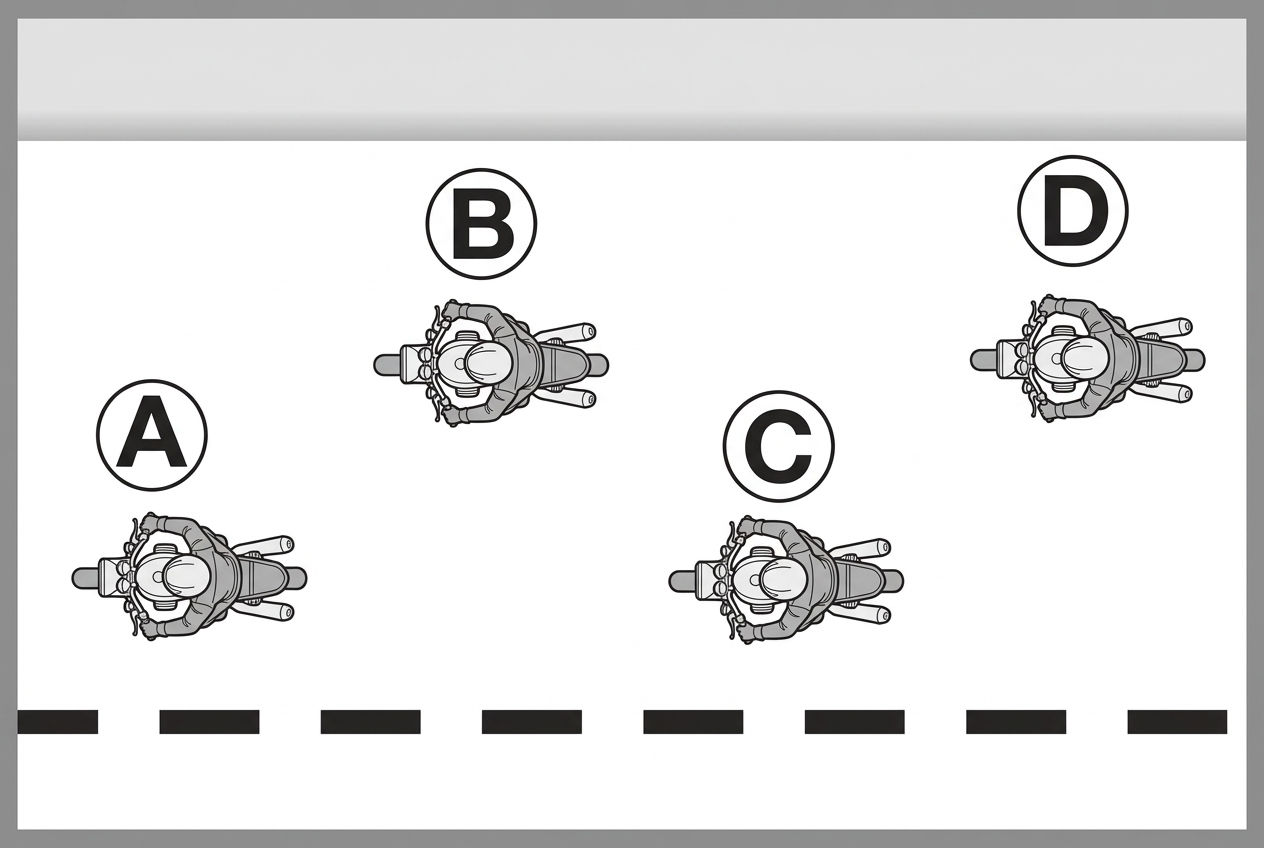
\includegraphics[width=0.8\linewidth]{ q_8.jpeg }
\captionof*{figure}{ Четыре мотоцикла (обозначенные буквами A, B, C, D) движутся в шахматном порядке по многополосной дороге: A — лидер в левой части, B — следует за лидером в правой части, C — третий, в левой части и позади лидера. }

\begin{itemize}[nosep,leftmargin=2em]
\item [A.] Четыре секунды.
\item [B.] Длина одного автомобиля.
\item [C.] Одна секунда.
\item [D.] Две секунды.

\end{itemize}
\end{minipage}


\begin{minipage}{\linewidth}
\vspace{1em}\noindent\textbf{9. Мотоциклисты, едущие в шахматном порядке, будут обгонять автомобиль. После того как лидер закончит обгон, он должен:}

\begin{itemize}[nosep,leftmargin=2em]
\item [A.] Занять правую часть полосы движения.
\item [B.] Занять центральную часть полосы движения.
\item [C.] Занять левую часть полосы движения.
\item [D.] Подать сигнал остальным, чтобы они следовали за ним.

\end{itemize}
\end{minipage}


\begin{minipage}{\linewidth}
\vspace{1em}\noindent\textbf{10. Алкоголь попадает в кровоток и быстро достигает мозга. На что это влияет в первую очередь?}

\begin{itemize}[nosep,leftmargin=2em]
\item [A.] Способность принимать адекватные решения.
\item [B.] Речь.
\item [C.] Чувство равновесия.
\item [D.] Зрение.

\end{itemize}
\end{minipage}


\begin{minipage}{\linewidth}
\vspace{1em}\noindent\textbf{11. Алкоголь в первую очередь влияет на:}

\begin{itemize}[nosep,leftmargin=2em]
\item [A.] Зрение.
\item [B.] Речь.
\item [C.] Способность принимать адекватные решения.
\item [D.] Чувство равновесия.

\end{itemize}
\end{minipage}


\begin{minipage}{\linewidth}
\vspace{1em}\noindent\textbf{12. Примерно половина всех смертельных случаев в результате ДТП с участием мотоциклов происходит по причине:}

\begin{itemize}[nosep,leftmargin=2em]
\item [A.] Состоянием дорог.
\item [B.] Шлемом мотоциклиста.
\item [C.] Из-за воздействия алкоголя.
\item [D.] Механическая неисправность.

\end{itemize}
\end{minipage}


\begin{minipage}{\linewidth}
\vspace{1em}\noindent\textbf{13. Если вы не контролируете количество выпитого:}

\begin{itemize}[nosep,leftmargin=2em]
\item [A.] Езжайте медленнее.
\item [B.] Перед поездкой выдержите как минимум час после каждой порции алкоголя.
\item [C.] Занимайтесь спортом или танцуйте, чтобы вывести алкоголь из организма.
\item [D.] Пейте горячий кофе, чтобы оставаться бодрым

\end{itemize}
\end{minipage}


\begin{minipage}{\linewidth}
\vspace{1em}\noindent\textbf{14. Исследования показывают, что почти половина всех мотоциклистов, погибших в ДТП:}

\begin{itemize}[nosep,leftmargin=2em]
\item [A.] Имели плохое зрение.
\item [B.] Употребляли алкоголь.
\item [C.] Превышали скорость.
\item [D.] Не обладали достаточным опытом

\end{itemize}
\end{minipage}


\begin{minipage}{\linewidth}
\vspace{1em}\noindent\textbf{15. Какое количество алкоголя начинает влять на способность ясно мыслить и безопасно управлять мотоциклом?}

\begin{itemize}[nosep,leftmargin=2em]
\item [A.] 1 порция алкоголя.
\item [B.] 6 порций алкоголя.
\item [C.] 3 порции алкоголя.
\item [D.] 2 порции алкоголя.

\end{itemize}
\end{minipage}


\begin{minipage}{\linewidth}
\vspace{1em}\noindent\textbf{16. Если вы выпьете 4 стандартных порции алкоголя, какое минимальное количество алкоголя останется в вашем организме через 2 часа?}

\begin{itemize}[nosep,leftmargin=2em]
\item [A.] 2 порции.
\item [B.] 3 порции.
\item [C.] 1 порция.
\item [D.] 4 порции.

\end{itemize}
\end{minipage}


\begin{minipage}{\linewidth}
\vspace{1em}\noindent\textbf{17. Для максимальной безопасности ваш шлем должен:}

\begin{itemize}[nosep,leftmargin=2em]
\item [A.] Плотно прилегать у основания; свободно — в верхней части.
\item [B.] Сидеть свободно по всему периметру.
\item [C.] Плотно прилегать по всему периметру.
\item [D.] Носить только во время длительных поездок.

\end{itemize}
\end{minipage}


\begin{minipage}{\linewidth}
\vspace{1em}\noindent\textbf{18. Самое важное, что вы можете сделать, чтобы повысить свои шансы на выживание при аварии это:}

\begin{itemize}[nosep,leftmargin=2em]
\item [A.] Опрокинуть мотоцикл до столкновения с препятствием.
\item [B.] Носить надежно закрепленный шлем.
\item [C.] Хорошо знать свой мотоцикл.
\item [D.] Ездить по центральной части полосы движения.

\end{itemize}
\end{minipage}


\begin{minipage}{\linewidth}
\vspace{1em}\noindent\textbf{19. Ношение шлема может снизить вероятность получения смертельной травмы головы при:}

\begin{itemize}[nosep,leftmargin=2em]
\item [A.] Только при столкновении на низкой скорости.
\item [B.] Только при ДТП с участием одного транспортного средства.
\item [C.] Любом ДТП, независимо от скорости.
\item [D.] Только при столкновениях на высокой скорости.

\end{itemize}
\end{minipage}


\begin{minipage}{\linewidth}
\vspace{1em}\noindent\textbf{20. Ношение шлема:}

\begin{itemize}[nosep,leftmargin=2em]
\item [A.] Снизит вероятность травм шеи и головы.
\item [B.] Увеличит вероятность травмы шеи.
\item [C.] Ухудшит обзор на две трети.
\item [D.] Ни уменьшит, ни увеличит вероятность травмы головы.

\end{itemize}
\end{minipage}


\begin{minipage}{\linewidth}
\vspace{1em}\noindent\textbf{21. Что из перечисленного ниже обеспечивает наилучшую защиту глаз и лица во время езды?}

\begin{itemize}[nosep,leftmargin=2em]
\item [A.] Защитные очки.
\item [B.] Ветровое стекло (щиток на мотоцикле).
\item [C.] Защитный щиток шлема.
\item [D.] Солнцезащитные очки.

\end{itemize}
\end{minipage}


\begin{minipage}{\linewidth}
\vspace{1em}\noindent\textbf{22. При езде на незнакомом мотоцикле:}

\begin{itemize}[nosep,leftmargin=2em]
\item [A.] Не переключайтесь выше третьей передачи.
\item [B.] Держитесь правой части полосы движения.
\item [C.] Попросите владельца поехать с вами.
\item [D.] Оставляйте больше дистанции для торможения.

\end{itemize}
\end{minipage}


\begin{minipage}{\linewidth}
\vspace{1em}\noindent\textbf{23. Аварийный выключатель двигателя обычно расположен:}

\begin{itemize}[nosep,leftmargin=2em]
\item [A.] Рядом с ручагом сцепления.
\item [B.] На левой ручке руля.
\item [C.] Рядом с правой ручкой
\item [D.] На верхней части топливного бака

\end{itemize}
\end{minipage}


\begin{minipage}{\linewidth}
\vspace{1em}\noindent\textbf{24. При правильной регулировке зеркала вы можете видеть:}

\begin{itemize}[nosep,leftmargin=2em]
\item [A.] Полосу движения рядом с вами.
\item [B.] Полосу движения позади вас.
\item [C.] Часть полосы движения рядом с вами и позади вас.
\item [D.] Всё, что находится сзади и сбоку.

\end{itemize}
\end{minipage}


\begin{minipage}{\linewidth}
\vspace{1em}\noindent\textbf{25. При замедлении перед обычной остановкой:}

\begin{itemize}[nosep,leftmargin=2em]
\item [A.] Используйте только задний тормоз.
\item [B.] Уменьшите подачу газа и используйте только передний тормоз.
\item [C.] При замедлении переключайтесь на более низкую передачу.
\item [D.] Выжмите сцепление и двигайтесь накатом.

\end{itemize}
\end{minipage}


\begin{minipage}{\linewidth}
\vspace{1em}\noindent\textbf{26. При повороте следует:}

\begin{itemize}[nosep,leftmargin=2em]
\item [A.] Следить за центральной линией.
\item [B.] Смотреть прямо вперед.
\item [C.] Смотреть на ограждение.
\item [D.] Смотреть вперед, в сторону поворота.

\end{itemize}
\end{minipage}


\begin{minipage}{\linewidth}
\vspace{1em}\noindent\textbf{27. Какое из следующих утверждений верно:}

\begin{itemize}[nosep,leftmargin=2em]
\item [A.] Нажмите на рукоять руля слева, наклонитесь влево, поедитете вправо.
\item [B.] Нажми с левой стороны, наклонись влево, поедешь влево.
\item [C.] Нажми с левой стороны, наклонись вправо, поедешь вправо.
\item [D.] Нажми с правой стороны, наклонись вправо, поедешь влево.

\end{itemize}
\end{minipage}


\begin{minipage}{\linewidth}
\vspace{1em}\noindent\textbf{28. Во время поворота лучше всего:}

\begin{itemize}[nosep,leftmargin=2em]
\item [A.] Сохранять постоянную скорость или плавно ускоряться.
\item [B.] Снизить скорость.
\item [C.] Использовать тормоза.
\item [D.] Ускоряться и смотреть прямо вперед.

\end{itemize}
\end{minipage}


\begin{minipage}{\linewidth}
\vspace{1em}\noindent\textbf{29. Если вам нужно замедлиться во время поворота:}

\begin{itemize}[nosep,leftmargin=2em]
\item [A.] Задействуйте задний тормоз и наклонитесь сильнее в сторону поворота.
\item [B.] Ни в коем случае не тормозите.
\item [C.] Аккуратно задействуйте оба тормоза.
\item [D.] Задействуйте только задний тормоз.

\end{itemize}
\end{minipage}


\begin{minipage}{\linewidth}
\vspace{1em}\noindent\textbf{30. Для обычной остановки используйте:}

\begin{itemize}[nosep,leftmargin=2em]
\item [A.] Сначала задний тормоз.
\item [B.] Оба тормоза и переключение на пониженную передачу.
\item [C.] Передний тормоз и переключение на пониженную передачу.
\item [D.] Только задний тормоз.

\end{itemize}
\end{minipage}


\begin{minipage}{\linewidth}
\vspace{1em}\noindent\textbf{31. У вашего мотоцикла два тормоза. Используйте оба тормоза:}

\begin{itemize}[nosep,leftmargin=2em]
\item [A.] Только при экстренной остановке.
\item [B.] При резком маневре.
\item [C.] Каждый раз, когда вы замедляетесь или останавливаетесь.
\item [D.] Только при обычной остановке.

\end{itemize}
\end{minipage}


\begin{minipage}{\linewidth}
\vspace{1em}\noindent\textbf{32. При обычном повороте:}

\begin{itemize}[nosep,leftmargin=2em]
\item [A.] Наклоняйте мотоцикл сильнее, чем тело.
\item [B.] Наклоняйте мотоцикл и тело под одинаковым углом.
\item [C.] Не наклоняйтесь.
\item [D.] Наклоняйте тело сильнее, чем мотоцикл.

\end{itemize}
\end{minipage}


\begin{minipage}{\linewidth}
\vspace{1em}\noindent\textbf{33. При медленных крутых поворотах:}

\begin{itemize}[nosep,leftmargin=2em]
\item [A.] Наклоняйте только мотоцикл, а тело держите прямо.
\item [B.] Наклоняйте тело сильнее, чем мотоцикл.
\item [C.] Наклоняйтесь вместе с мотоциклом.
\item [D.] Не наклоняйтесь.

\end{itemize}
\end{minipage}


\begin{minipage}{\linewidth}
\vspace{1em}\noindent\textbf{34. Чтобы снизить скорость перед поворотом:}

\begin{itemize}[nosep,leftmargin=2em]
\item [A.] Переключитесь на нейтраль.
\item [B.] Зажмите сцепление и задействуйте оба тормоза.
\item [C.] Используйте только задний тормоз.
\item [D.] Закройте дроссель и задействуйте оба тормоза.

\end{itemize}
\end{minipage}


\begin{minipage}{\linewidth}
\vspace{1em}\noindent\textbf{35. При повороте важно:}

\begin{itemize}[nosep,leftmargin=2em]
\item [A.] Смотрите прямо вперед.
\item [B.] Снизить скорость после входа в поворот.
\item [C.] Снизить скорость при выходе из поворота.
\item [D.] Смотреть сквозь поворот туда, куда вы хотите ехать.

\end{itemize}
\end{minipage}


\begin{minipage}{\linewidth}
\vspace{1em}\noindent\textbf{36. Важно искать на дороге пути отхода:}

\begin{itemize}[nosep,leftmargin=2em]
\item [A.] Через переулки.
\item [B.] На перекрестках.
\item [C.] При езде на одолженном мотоцикле.
\item [D.] На поворотах.

\end{itemize}
\end{minipage}


\begin{minipage}{\linewidth}
\vspace{1em}\noindent\textbf{37. Чтобы правильно принимать решения в дорожном движении, сначала нужно:}

\begin{itemize}[nosep,leftmargin=2em]
\item [A.] Уметь резко сворачивать.
\item [B.] Смотреть вперёд.
\item [C.] Следить за пешеходами.
\item [D.] Уметь быстро останавливаться.

\end{itemize}
\end{minipage}


\begin{minipage}{\linewidth}
\vspace{1em}\noindent\textbf{38. Водитель автомобиля подаёт сигнал о повороте налево. Мотоциклист должен:}

\vspace{1ex}
\centering
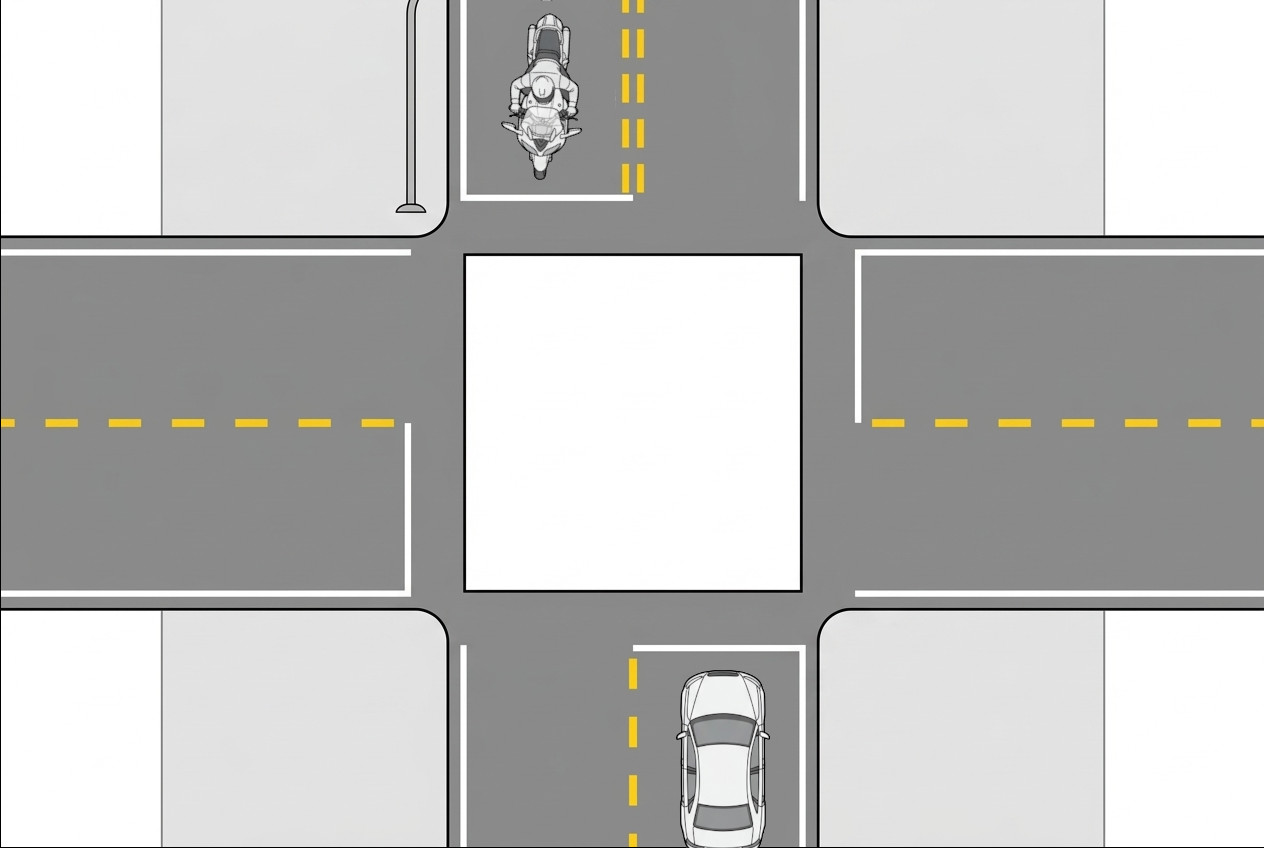
\includegraphics[width=0.8\linewidth]{ q_38.jpeg }
\captionof*{figure}{ Сцена на перекрёстке, где мотоцикл и автомобиль встречаются на перекрёстке. Мотоцикл движется прямо, а автомобиль поворачивает перед мотоциклом. Мотоцикл имеет преимущество в движении. }

\begin{itemize}[nosep,leftmargin=2em]
\item [A.] Сохранять скорость и держаться в центре полосы движения.
\item [B.] Снизить скорость и держаться подальше от приближающихся транспортных средств.
\item [C.] Увеличить скорость и двигаться влево.
\item [D.] Увеличить скорость и оставаться в центре полосы движения.

\end{itemize}
\end{minipage}


\begin{minipage}{\linewidth}
\vspace{1em}\noindent\textbf{39. Вам следует уделять особое внимание проверке обстановки сзади:}

\begin{itemize}[nosep,leftmargin=2em]
\item [A.] Перед входом в поворот.
\item [B.] При приближении к перекрёстку.
\item [C.] Когда везёте пассажира.
\item [D.] Перед тем, как снизить скорость.

\end{itemize}
\end{minipage}


\begin{minipage}{\linewidth}
\vspace{1em}\noindent\textbf{40. При подготовке к обгону обычно лучше:}

\begin{itemize}[nosep,leftmargin=2em]
\item [A.] Подать сигнал, посмотреть в левое зеркало,  посмотреть налево повернув голову.
\item [B.] Подать сигнал, перестроиться в левый ряд, ускориться.
\item [C.] Подать сигнал, посмотреть в левое зеркало.
\item [D.] Включить поворотник, посмотреть в левое зеркало, ускориться.

\end{itemize}
\end{minipage}


\begin{minipage}{\linewidth}
\vspace{1em}\noindent\textbf{41. Движение по центру полосы:}

\begin{itemize}[nosep,leftmargin=2em]
\item [A.] Мешает другим участникам движения увидеть вас.
\item [B.] Является самым безопасным местом при приближении к перекрёсткам.
\item [C.] Не позволяет другим транспортным средствам занимать вашу полосу.
\item [D.] По возможности следует избегать.

\end{itemize}
\end{minipage}


\begin{minipage}{\linewidth}
\vspace{1em}\noindent\textbf{42. Чтобы предотвратить попытки других водителей занять вашу полосу вместе с вами, обычно лучше всего:}

\begin{itemize}[nosep,leftmargin=2em]
\item [A.] Двигаться по левой части полосы.
\item [B.] Двигаться по центральной части полосы.
\item [C.] Ехать рядом с другим транспортным средством.
\item [D.] Двигаться по правой части полосы.

\end{itemize}
\end{minipage}


\begin{minipage}{\linewidth}
\vspace{1em}\noindent\textbf{43. Поддержание зоны безопасности (пространственного буфера) вокруг мотоцикла:}

\begin{itemize}[nosep,leftmargin=2em]
\item [A.] Необходимо только начинающим мотоциклистам.
\item [B.] Даёт вам время и пространство для реакции.
\item [C.] Позволяет лавировать в потоке при необходимости.
\item [D.] Делает вас более уязвимым.

\end{itemize}
\end{minipage}


\begin{minipage}{\linewidth}
\vspace{1em}\noindent\textbf{44. Чтобы вовремя заметить встречный транспорт и сохранить зону безопасности, как показано на иллюстрации выше:}

\vspace{1ex}
\centering
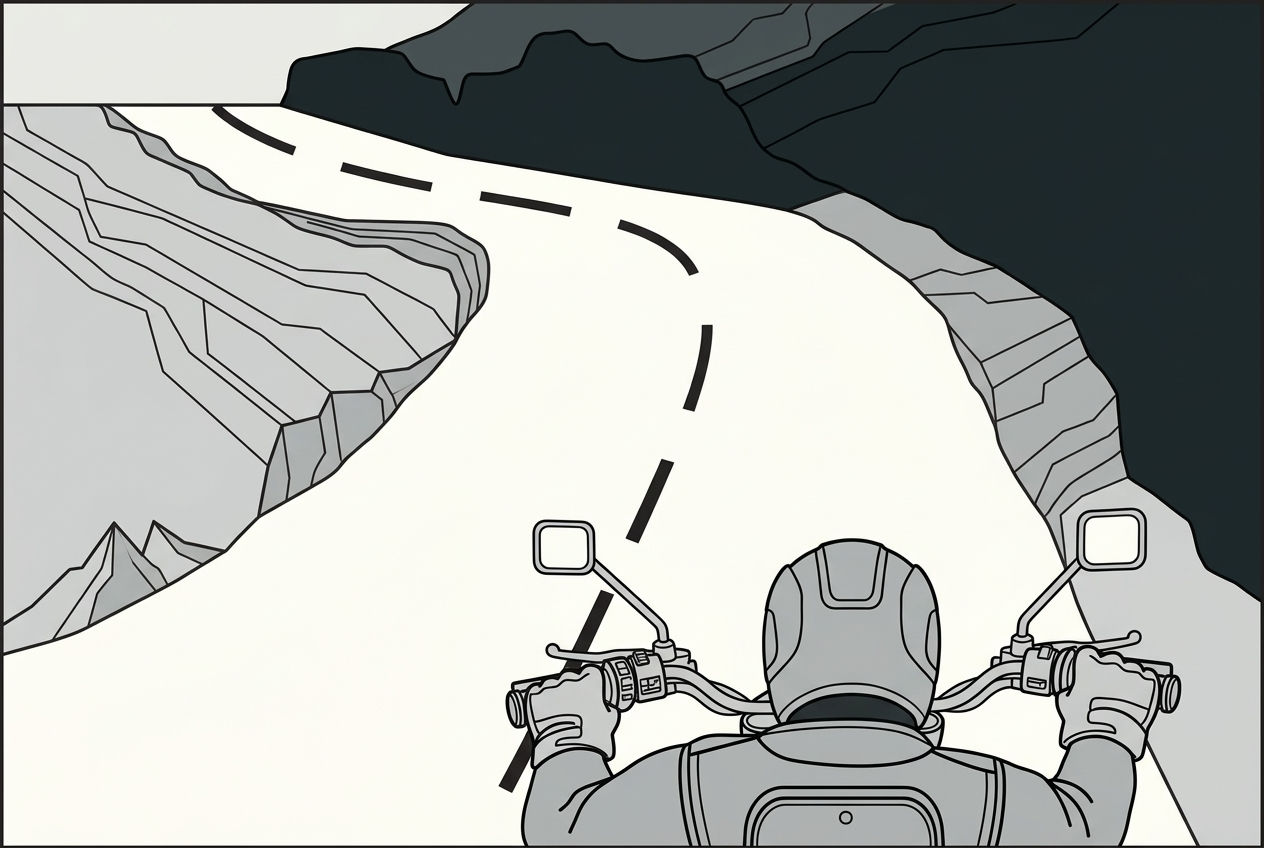
\includegraphics[width=0.8\linewidth]{ q_44.jpeg }
\captionof*{figure}{ Вид вперёд на извилистую дорогу }

\begin{itemize}[nosep,leftmargin=2em]
\item [A.] Двигайтесь по центру полосы.
\item [B.] Сместитесь вправо и отклонитесь в сторону, противоположную повороту.
\item [C.] Не наклоняйте мотоцикл.
\item [D.] Двигайтесь по левой части полосы.

\end{itemize}
\end{minipage}


\begin{minipage}{\linewidth}
\vspace{1em}\noindent\textbf{45. Вы планируете повернуть направо после остановки на перекрёстке. Обычно лучше всего:}

\begin{itemize}[nosep,leftmargin=2em]
\item [A.] Позволить авто сзади, объехать вас.
\item [B.] Выполнять поворот из центральной части полосы.
\item [C.] Выполнять поворот из правой части полосы.
\item [D.] Выполнять поворот из левой части полосы.

\end{itemize}
\end{minipage}


\begin{minipage}{\linewidth}
\vspace{1em}\noindent\textbf{46. Движение на близкой дистанции за впереди идущим транспортом:}

\begin{itemize}[nosep,leftmargin=2em]
\item [A.] Помогает видеть опасности на дороге.
\item [B.] Безопаснее в ночное время.
\item [C.] Защищает вас при плотном движении.
\item [D.] Является одной из причин ДТП по вине мотоциклистов.

\end{itemize}
\end{minipage}


\begin{minipage}{\linewidth}
\vspace{1em}\noindent\textbf{47. Двигаясь за автомобилем, вам следует стараться:}

\begin{itemize}[nosep,leftmargin=2em]
\item [A.] Ехать так, чтобы водитель видел вас в зеркало заднего вида.
\item [B.] Ехать рядом с другим автомобилем, чтобы быть заметнее.
\item [C.] Двигаться по левой стороне полосы.
\item [D.] Двигаться по правой стороне полосы.

\end{itemize}
\end{minipage}


\begin{minipage}{\linewidth}
\vspace{1em}\noindent\textbf{48. Самой частой причиной ДТП с участием мотоциклов и автомобилей на перекрёстках является:}

\begin{itemize}[nosep,leftmargin=2em]
\item [A.] Нарушение водителями преимущественного права проезда мотоциклиста.
\item [B.] То, что мотоциклистов не замечают выезжающие со второстепенных улиц автомобили.
\item [C.] Несоблюдение водителями дистанции позади мотоциклиста.
\item [D.] Непредоставление мотоциклистами преимущества встречному транспорту.

\end{itemize}
\end{minipage}


\begin{minipage}{\linewidth}
\vspace{1em}\noindent\textbf{49. ДТП с участием автомобилей и мотоциклов чаще всего происходят:}

\begin{itemize}[nosep,leftmargin=2em]
\item [A.] На перекрёстках.
\item [B.] Ночью.
\item [C.] При превышении скорости мотоциклистом.
\item [D.] На автомагистралях.

\end{itemize}
\end{minipage}


\begin{minipage}{\linewidth}
\vspace{1em}\noindent\textbf{50. Зрительный контакт с водителем на перекрёстке:}

\begin{itemize}[nosep,leftmargin=2em]
\item [A.] Является верным признаком того, что водитель, скорее всего, уступит дорогу.
\item [B.] Важен, если водитель выезжает со второстепенной улицы.
\item [C.] Не означает, что водитель действительно вас видит.
\item [D.] Вводит водителя в заблуждение.

\end{itemize}
\end{minipage}


\begin{minipage}{\linewidth}
\vspace{1em}\noindent\textbf{51. Наибольшая опасность для мотоциклиста при проезде мимо припаркованных автомобилей — это:}

\begin{itemize}[nosep,leftmargin=2em]
\item [A.] Автомобиль, заезжающий на парковочное место задним ходом.
\item [B.] Автомобиль, выезжающий с парковки на дорогу.
\item [C.] Открывающаяся дверь автомобиля.
\item [D.] Пешеход, выходящий из-за припаркованных машин.

\end{itemize}
\end{minipage}


\begin{minipage}{\linewidth}
\vspace{1em}\noindent\textbf{52. На этом рисунке световой сигнал, который скорее всего сделает мотоцикл заметным для водителя автомобиля — это:}

\vspace{1ex}
\centering
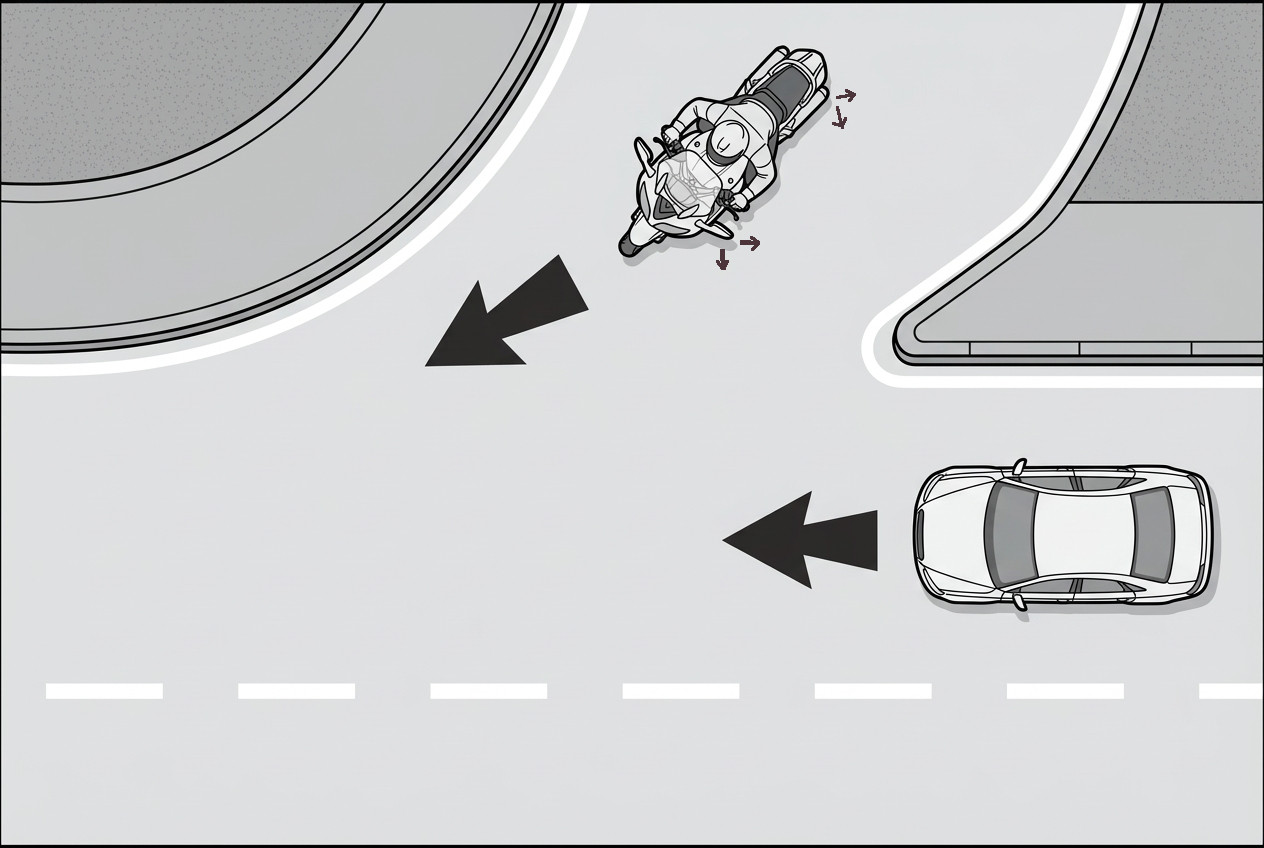
\includegraphics[width=0.8\linewidth]{ q_52.jpeg }
\captionof*{figure}{ Мотоциклист выезжает на шоссе, когда по правой полосе едет автомобиль }

\begin{itemize}[nosep,leftmargin=2em]
\item [A.] Стоп-сигнал.
\item [B.] Задний габаритный огонь.
\item [C.] Фара.
\item [D.] Указатель поворота.

\end{itemize}
\end{minipage}


\begin{minipage}{\linewidth}
\vspace{1em}\noindent\textbf{53. При движении в потоке ночью лучший способ обнаружить неровности на дороге — это:}

\begin{itemize}[nosep,leftmargin=2em]
\item [A.] Смотреть поверх едущих впереди автомобилей.
\item [B.] Включить дальний свет фар.
\item [C.] Следить за дорожными знаками.
\item [D.] Следить за задними габаритными огнями впереди идущего автомобиля.

\end{itemize}
\end{minipage}


\begin{minipage}{\linewidth}
\vspace{1em}\noindent\textbf{54. Лучший способ сделать ваш мотоцикл заметнее для других — это:}

\begin{itemize}[nosep,leftmargin=2em]
\item [A.] Двигаться по левой части полосы.
\item [B.] Надевать белый шлем.
\item [C.] Держаться в центральной части полосы.
\item [D.] Ездить с включённой фарой.

\end{itemize}
\end{minipage}


\begin{minipage}{\linewidth}
\vspace{1em}\noindent\textbf{55. Забытый включённый указатель поворота скорее всего:}

\begin{itemize}[nosep,leftmargin=2em]
\item [A.] Спровоцирует других водителей выехать на вашу траекторию движения.
\item [B.] Помешает другим заметить ваш стоп-сигнал.
\item [C.] Снизит вероятность аварии, так как другие водители будут держаться подальше.
\item [D.] Заставит других ехать слишком близко за вами.

\end{itemize}
\end{minipage}


\begin{minipage}{\linewidth}
\vspace{1em}\noindent\textbf{56. Особенно важно проверять зеркала заднего вида:}

\begin{itemize}[nosep,leftmargin=2em]
\item [A.] В дальних поездках.
\item [B.] При проезде перекрёстка.
\item [C.] При движении за другим транспортным средством.
\item [D.] Перед замедлением или остановкой.

\end{itemize}
\end{minipage}


\begin{minipage}{\linewidth}
\vspace{1em}\noindent\textbf{57. Перед перестроением на левую полосу:}

\begin{itemize}[nosep,leftmargin=2em]
\item [A.] Проверьте левое зеркало и поверните голову влево для проверки слепой зоны.
\item [B.] Проверьте правое зеркало, затем левое.
\item [C.] Проверьте левое зеркало, затем правое.
\item [D.] Подайте звуковой сигнал и ускорьтесь.

\end{itemize}
\end{minipage}


\begin{minipage}{\linewidth}
\vspace{1em}\noindent\textbf{58. Лучшая экипировка, чтобы быть заметным ночью — это:}

\begin{itemize}[nosep,leftmargin=2em]
\item [A.] Флуоресцентная одежда.
\item [B.] Белый шлем.
\item [C.] Одежда со световозвращающими элементами.
\item [D.] Красная куртка.

\end{itemize}
\end{minipage}


\begin{minipage}{\linewidth}
\vspace{1em}\noindent\textbf{59. Чтобы лучше видеть дорогу при движении за автомобилем ночью:}

\begin{itemize}[nosep,leftmargin=2em]
\item [A.] Увеличьте дистанцию и используйте ближний свет.
\item [B.] Используйте свет фар впереди идущего автомобиля.
\item [C.] Совершите обгон при безопасности и включите дальний свет.
\item [D.] Отстаньте подальше и включите дальний свет.

\end{itemize}
\end{minipage}


\begin{minipage}{\linewidth}
\vspace{1em}\noindent\textbf{60. При езде в ночное время:}

\begin{itemize}[nosep,leftmargin=2em]
\item [A.] Всегда двигайтесь по центральной полосе.
\item [B.] Ездите с включённой аварийной сигнализацией.
\item [C.] Носите световозвращающую одежду.
\item [D.] Держитесь ближе к едущему впереди транспорту для безопасности.

\end{itemize}
\end{minipage}


\begin{minipage}{\linewidth}
\vspace{1em}\noindent\textbf{61. Если при остановке вы заблокировали переднее колесо:}

\begin{itemize}[nosep,leftmargin=2em]
\item [A.] Отпустить задний тормоз.
\item [B.] Держать передний тормоз заблокированным до полной остановки.
\item [C.] Держать заблокированными оба тормоза.
\item [D.] Отпустить и снова нажать передний тормоз.

\end{itemize}
\end{minipage}


\begin{minipage}{\linewidth}
\vspace{1em}\noindent\textbf{62. На рисунке выше при попытке экстренной остановки заблокировалось заднее колесо. Как правило, лучше всего:}

\vspace{1ex}
\centering
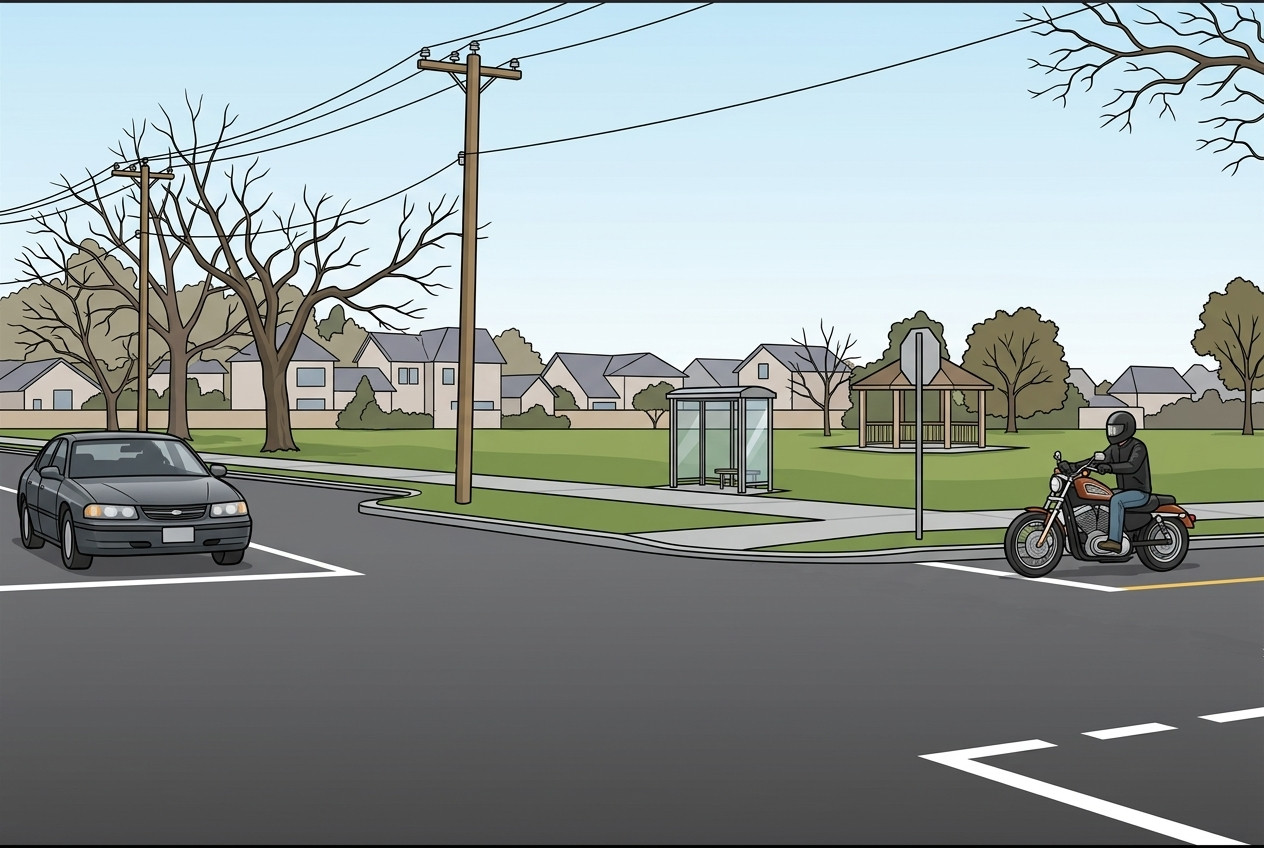
\includegraphics[width=0.8\linewidth]{ q_62.jpeg }
\captionof*{figure}{ Перекресток улиц в пригородном районе: слева автомобиль, справа мотоцикл, приближающиеся друг к другу. }

\begin{itemize}[nosep,leftmargin=2em]
\item [A.] Сохранять положение и отпустить задний тормоз.
\item [B.] Наклонить мотоцикл и отпустить задний тормоз.
\item [C.] Отпустить передний тормоз и держать задний тормоз заблокированным.
\item [D.] Держать заднее колесо заблокированным до полной остановки.

\end{itemize}
\end{minipage}


\begin{minipage}{\linewidth}
\vspace{1em}\noindent\textbf{63. При резком объезде препятствия важно:}

\begin{itemize}[nosep,leftmargin=2em]
\item [A.] Всегда тормозить перед объездом.
\item [B.] Разделять торможение и маневр.
\item [C.] Всегда тормозить после маневра.
\item [D.] Сворачивать в сторону движения опасности.

\end{itemize}
\end{minipage}


\begin{minipage}{\linewidth}
\vspace{1em}\noindent\textbf{64. Для проезда по металлическим решетчатым настилам моста:}

\begin{itemize}[nosep,leftmargin=2em]
\item [A.] Двигаться прямо.
\item [B.] Двигаться зигзагом.
\item [C.] Пересекать под острым углом, не меняя полосы.
\item [D.] Увеличить скорость.

\end{itemize}
\end{minipage}


\begin{minipage}{\linewidth}
\vspace{1em}\noindent\textbf{65. При переезде через предмет на дороге:}

\begin{itemize}[nosep,leftmargin=2em]
\item [A.] Оставаться в сиденье, пока не переедете его.
\item [B.] Приподняться над сиденьем.
\item [C.] Переезжать его по самому краю.
\item [D.] Сжать бензобак коленями.

\end{itemize}
\end{minipage}


\begin{minipage}{\linewidth}
\vspace{1em}\noindent\textbf{66. При проезде препятствия лучше всего:}

\begin{itemize}[nosep,leftmargin=2em]
\item [A.] Сохранять обычную посадку.
\item [B.] Приподняться над сиденьем.
\item [C.] Сжать бензобак коленями.
\item [D.] Максимально наклониться вперед.

\end{itemize}
\end{minipage}


\begin{minipage}{\linewidth}
\vspace{1em}\noindent\textbf{67. На двухполосной дороге с твердым покрытием песок и гравий чаще всего скапливаются:}

\begin{itemize}[nosep,leftmargin=2em]
\item [A.] В левой колее.
\item [B.] Ближе к центру дороги.
\item [C.] У краев дороги (у обочин).
\item [D.] По центру полосы.

\end{itemize}
\end{minipage}


\begin{minipage}{\linewidth}
\vspace{1em}\noindent\textbf{68. На мокрой дороге наиболее скользко обычно:}

\begin{itemize}[nosep,leftmargin=2em]
\item [A.] На мелком гравии.
\item [B.] В левой колее.
\item [C.] В правой колее.
\item [D.] В центральной части полосы.

\end{itemize}
\end{minipage}


\begin{minipage}{\linewidth}
\vspace{1em}\noindent\textbf{69. Чтобы безопасно проехать скользкий участок дороги, лучше всего:}

\begin{itemize}[nosep,leftmargin=2em]
\item [A.] Легко притормаживать задним тормозом во время движения по нему.
\item [B.] Снизить скорость до въезда на него.
\item [C.] Постепенно ускоряться.
\item [D.] Переключиться на пониженную передачу при въезде на него.

\end{itemize}
\end{minipage}


\begin{minipage}{\linewidth}
\vspace{1em}\noindent\textbf{70. Для остановки на мокром асфальте:}

\begin{itemize}[nosep,leftmargin=2em]
\item [A.] Использовать передний тормоз только если колесо начинает скользить.
\item [B.] Двигаться накатом до полной остановки.
\item [C.] Использовать только задний тормоз.
\item [D.] Использовать передний и задний тормоза одновременно.

\end{itemize}
\end{minipage}


\begin{minipage}{\linewidth}
\vspace{1em}\noindent\textbf{71. При движении по дорогам с твердым покрытием в местах скопления песка и гравия следует:}

\begin{itemize}[nosep,leftmargin=2em]
\item [A.] Переключиться на пониженную передачу и добавить газ.
\item [B.] Выжать сцепление.
\item [C.] Использовать только задний тормоз для замедления.
\item [D.] Избегать резких изменений скорости или направления движения.

\end{itemize}
\end{minipage}


\begin{minipage}{\linewidth}
\vspace{1em}\noindent\textbf{72. Если спущено заднее колесо:}

\begin{itemize}[nosep,leftmargin=2em]
\item [A.] Вы не сможете сохранить контроль.
\item [B.] Вы потеряете передачу мощности на заднее колесо.
\item [C.] Задняя часть мотоцикла будет вилять из стороны в сторону.
\item [D.] Рулевое управление станет «тяжелым».

\end{itemize}
\end{minipage}


\begin{minipage}{\linewidth}
\vspace{1em}\noindent\textbf{73. Если во время движения у вас пробило колесо, крепко держитесь за руль и:}

\begin{itemize}[nosep,leftmargin=2em]
\item [A.] Плавно задействуйте оба тормоза.
\item [B.] Используйте тормоз исправного колеса или избегайте торможения.
\item [C.] Продолжайте движение до ближайшей мастерской.
\item [D.] Используйте только тормоз спущенного колеса.

\end{itemize}
\end{minipage}


\begin{minipage}{\linewidth}
\vspace{1em}\noindent\textbf{74. Если во время движения спущено переднее колесо:}

\begin{itemize}[nosep,leftmargin=2em]
\item [A.] Используйте передний тормоз.
\item [B.] Вы не сможете управлять мотоциклом.
\item [C.] Используйте задний тормоз и съедьте к краю дороги.
\item [D.] Поверните вправо и примените оба тормоза.

\end{itemize}
\end{minipage}


\begin{minipage}{\linewidth}
\vspace{1em}\noindent\textbf{75. При спущенном переднем колесе:}

\begin{itemize}[nosep,leftmargin=2em]
\item [A.] Рулевое управление станет тяжелым.
\item [B.] Это никак не повлияет на управляемость.
\item [C.] Задняя часть мотоцикла будет вилять из стороны в сторону.
\item [D.] Вы потеряете эффективность тормозов.

\end{itemize}
\end{minipage}


\begin{minipage}{\linewidth}
\vspace{1em}\noindent\textbf{76. Если заклинило ручку газа:}

\begin{itemize}[nosep,leftmargin=2em]
\item [A.] Выжмите сцепление и используйте аварийный выключатель двигателя.
\item [B.] Переключитесь на нейтраль и примените оба тормоза.
\item [C.] Переключитесь на пониженную передачу и примените оба тормоза.
\item [D.] Используйте передний тормоз.

\end{itemize}
\end{minipage}


\begin{minipage}{\linewidth}
\vspace{1em}\noindent\textbf{77. На рисунке выше обычно лучше всего:}

\vspace{1ex}
\centering
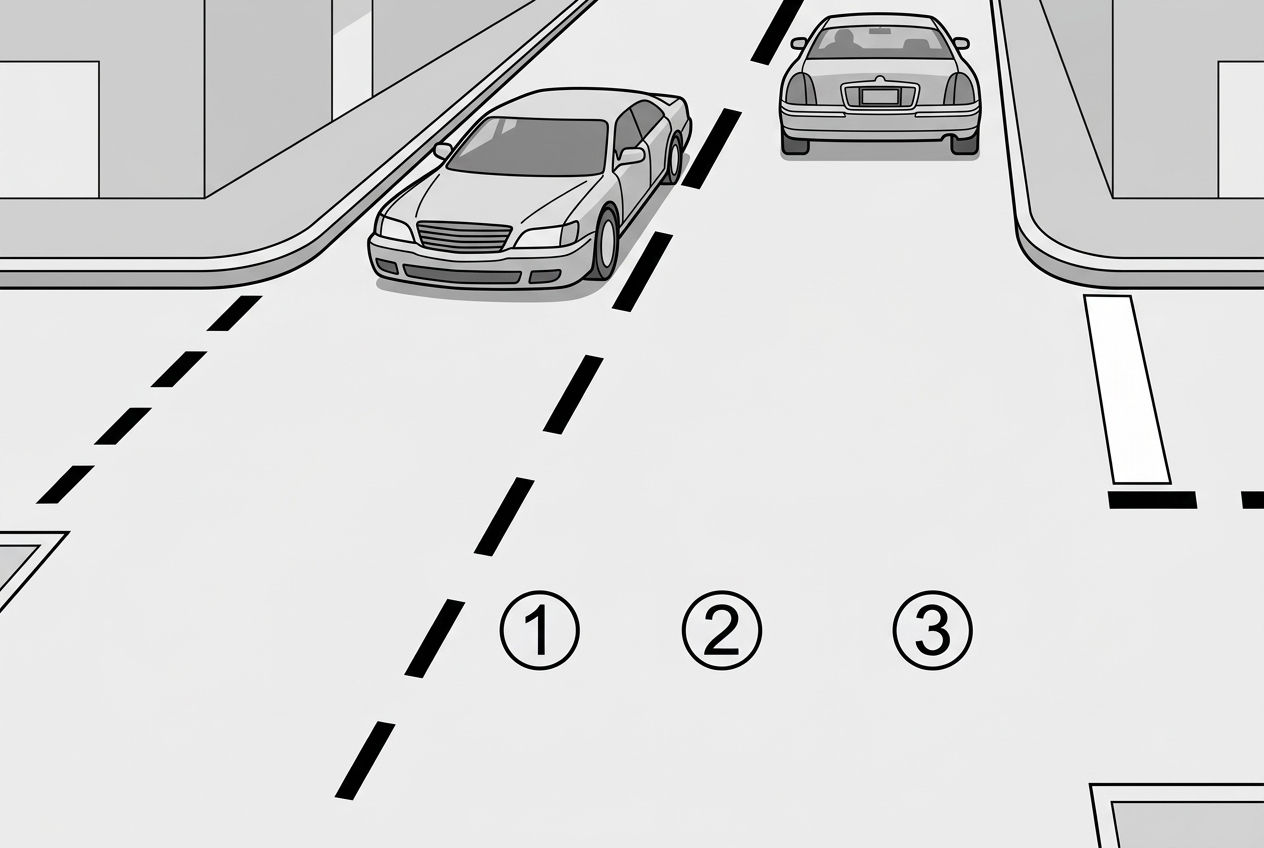
\includegraphics[width=0.8\linewidth]{ q_77.jpeg }
\captionof*{figure}{ Иллюстрация полосы движения с тремя пронумерованными частями: 1 — левая, 2 — центральная, 3 — правая. }

\begin{itemize}[nosep,leftmargin=2em]
\item [A.] Увеличить скорость, чтобы быстро проехать.
\item [B.] Двигаться в позиции 3.
\item [C.] Двигаться в позиции 1.
\item [D.] Двигаться в позиции 2 или 3.

\end{itemize}
\end{minipage}


\begin{minipage}{\linewidth}
\vspace{1em}\noindent\textbf{78. На этом рисунке A, B и C едут в группе. Для обгона мотоциклист B должен:}

\vspace{1ex}
\centering
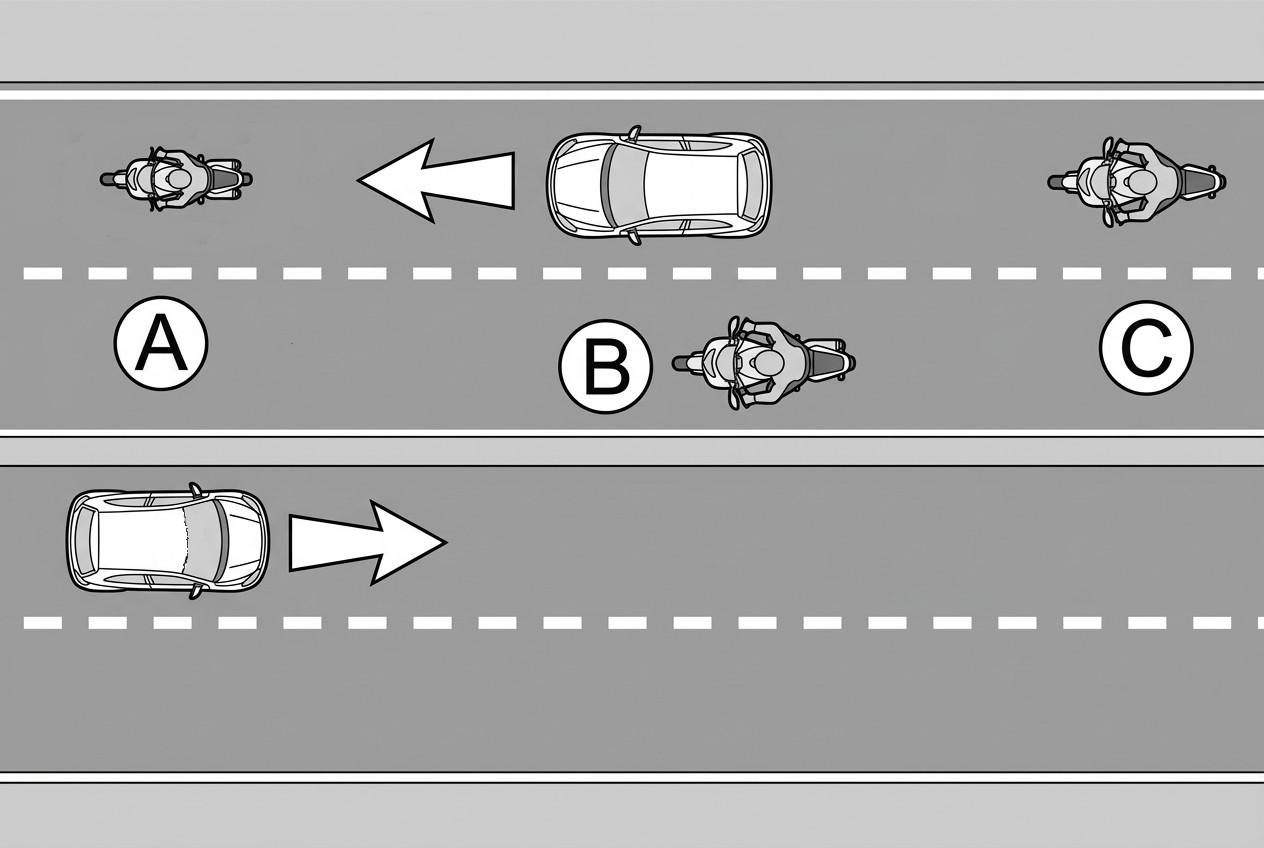
\includegraphics[width=0.8\linewidth]{ q_78.jpeg }
\captionof*{figure}{ Иллюстрация группы мотоциклов, обгоняющих автомобиль: A уже завершил обгон, B совершает обгон, C ожидает. }

\begin{itemize}[nosep,leftmargin=2em]
\item [A.] Завершить обгон перед мотоциклистом A.
\item [B.] Совершать обгон одновременно с C.
\item [C.] Вернуться в полосу и ехать рядом с A.
\item [D.] Вернуться в правую часть полосы позади A.

\end{itemize}
\end{minipage}


\begin{minipage}{\linewidth}
\vspace{1em}\noindent\textbf{79. Чтобы создать больше пространства в ситуации, изображенной выше, вам следует:}

\vspace{1ex}
\centering
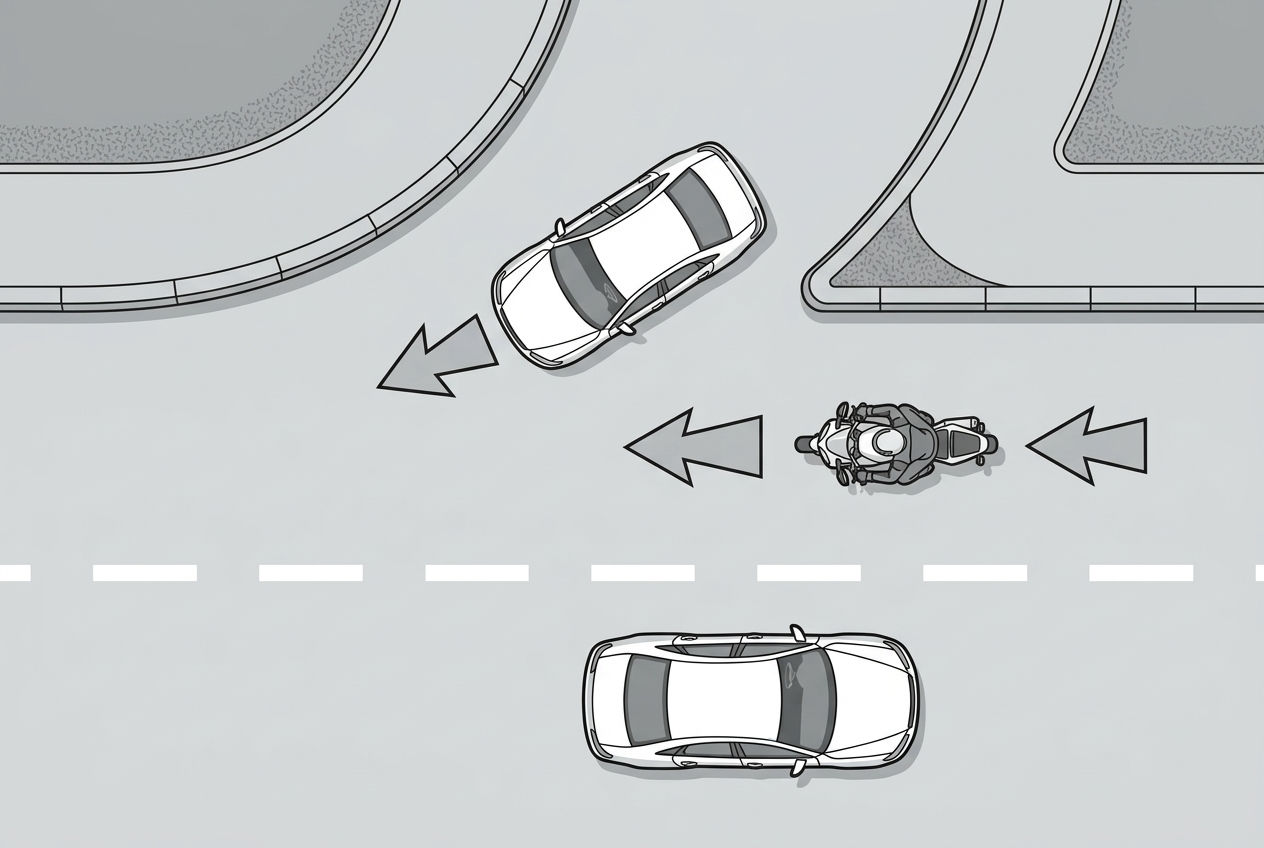
\includegraphics[width=0.8\linewidth]{ q_79.jpeg }
\captionof*{figure}{ Мотоцикл едет по правой полосе шоссе, автомобиль перестраивается в правую полосу перед мотоциклом. }

\begin{itemize}[nosep,leftmargin=2em]
\item [A.] Ехать в правой части полосы.
\item [B.] Скорректировать скорость и оставаться по центру полосы.
\item [C.] Перестроиться в левую полосу.
\item [D.] Обогнать автомобиль слева от вас.

\end{itemize}
\end{minipage}


\begin{minipage}{\linewidth}
\vspace{1em}\noindent\textbf{80. Большинство аварий с участием мотоцикла и автомобиля:}

\begin{itemize}[nosep,leftmargin=2em]
\item [A.] Происходят из-за того, что водитель автомобиля выезжает на траекторию движения мотоцикла.
\item [B.] Приводят к незначительным травмам.
\item [C.] Происходят из-за того, что мотоциклист поворачивает налево перед транспортным средством.
\item [D.] Происходят из-за превышения скорости.

\end{itemize}
\end{minipage}


\begin{minipage}{\linewidth}
\vspace{1em}\noindent\textbf{81. Вы собираетесь перестроиться в левую полосу, как показано на рисунке выше. Чтобы заметить автомобили, проезжающие рядом с вами, лучше всего:}

\vspace{1ex}
\centering
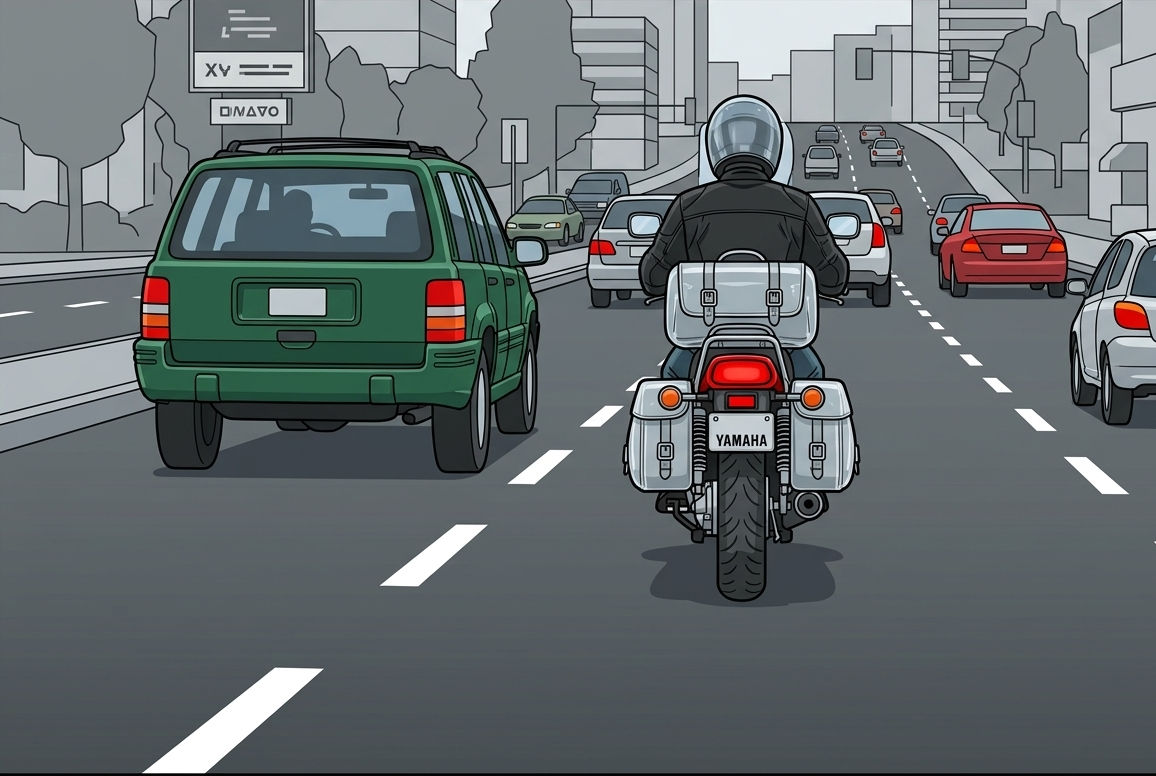
\includegraphics[width=0.8\linewidth]{ q_81.jpeg }
\captionof*{figure}{ Мотоцикл по центру средней полосы, готовится к перестроению в левую полосу. }

\begin{itemize}[nosep,leftmargin=2em]
\item [A.] Замедлиться и посмотреть в левое зеркало.
\item [B.] Посмотреть в левое зеркало.
\item [C.] Ускориться и посмотреть в левое зеркало.
\item [D.] Повернуть голову влево.

\end{itemize}
\end{minipage}


\begin{minipage}{\linewidth}
\vspace{1em}\noindent\textbf{82. Чтобы подстроиться под дорожное движение и избежать мусора на повороте, показанном на рисунке, следует ехать:}

\vspace{1ex}
\centering

\includegraphics[width=0.8\linewidth]{ q_82.jpeg }
\captionof*{figure}{ Поворот дороги без разделительного барьера, где правая сторона имеет пронумерованные части: 1 — левая часть, 2 — центральная часть, 3 — правая часть. }

\begin{itemize}[nosep,leftmargin=2em]
\item [A.] В позиции 3.
\item [B.] В позиции 2.
\item [C.] Без наклона.
\item [D.] В позиции 1.

\end{itemize}
\end{minipage}


\begin{minipage}{\linewidth}
\vspace{1em}\noindent\textbf{83. Чтобы пересечь рельсы, идущие параллельно вашему курсу:}

\begin{itemize}[nosep,leftmargin=2em]
\item [A.] Постепенно переезжать их под острым углом.
\item [B.] Выехать на встречную полосу, чтобы пересечь их под углом 90 градусов.
\item [C.] Подождать, пока рельсы закончатся.
\item [D.] Отъехать в сторону, затем повернуть и пересечь их под углом не менее 45 градусов.

\end{itemize}
\end{minipage}


\begin{minipage}{\linewidth}
\vspace{1em}\noindent\textbf{84. На этом рисунке мотоциклист, находящийся в наиболее опасном положении, это:}

\vspace{1ex}
\centering
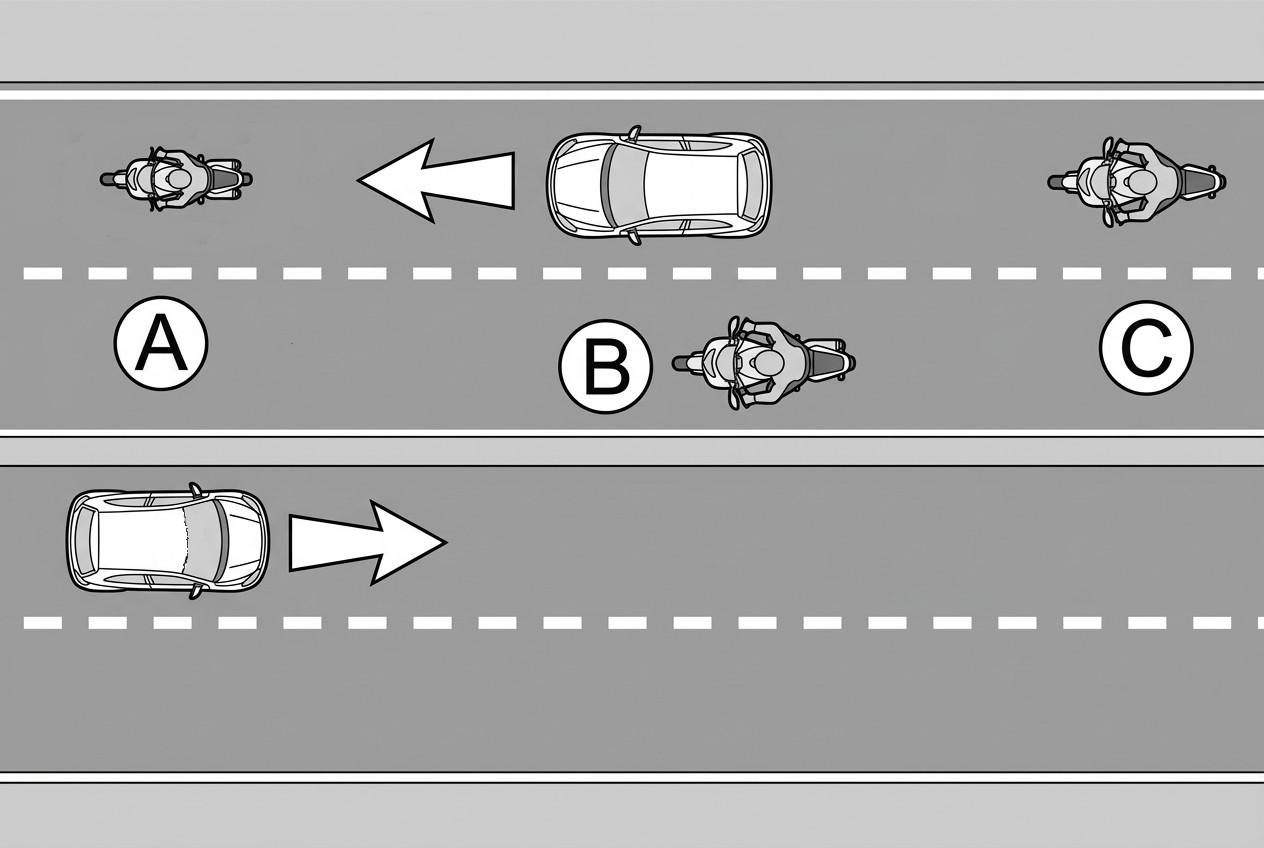
\includegraphics[width=0.8\linewidth]{ q_84.jpeg }
\captionof*{figure}{ Иллюстрация группы мотоциклистов, обгоняющих автомобиль: A уже завершил обгон, B совершает обгон, C ожидает. }

\begin{itemize}[nosep,leftmargin=2em]
\item [A.] Мотоциклист B.
\item [B.] Мотоциклист C.
\item [C.] Мотоциклист A.
\item [D.] Никто.

\end{itemize}
\end{minipage}


	
\end{multicols}


\clearpage
\subsection{\ru{Ответы с пояснениями RU}}	
\begin{multicols}{2}
	\raggedcolumns
	\begin{minipage}{\linewidth}
\noindent\textbf{1.}  -- \textbf {(B).} Регулировка зеркал при перевозке пассажира. Пассажир должен:  \textbf {Сесть на сиденье рядом с вами.} \par \textit {Вес пассажира влияет на подвеску мотоцикла и вашу позу, поэтому зеркала необходимо настраивать, когда вы оба сидите на байке.} \\
\end{minipage}

\begin{minipage}{\linewidth}
\noindent\textbf{2.}  -- \textbf {(C).} Пассажир должен:  \textbf {Держаться за талию водителя.} \par \textit {Держась за талию водителя (или за бедра/пояс), пассажир будет синхронно двигаться и наклоняться вместе с водителем, обеспечивая устойчивость байка. Даже если вам от этого неловко.} \\
\end{minipage}

\begin{minipage}{\linewidth}
\noindent\textbf{3.}  -- \textbf {(A).} Когда мотоцикл останавливается на перекрёстке, пассажир должен:  \textbf {Держать ноги на подножках.} \par \textit {Если пасажир будет двигаться или опустит ноги на землю это может нарушить равновесие мотоцикла и создать риск получения травмы, поэтому во время остановки только водитель должен контролировать баланс и равновесие мотоцикла.} \\
\end{minipage}

\begin{minipage}{\linewidth}
\noindent\textbf{4.}  -- \textbf {(C).} При езде с пассажиром:  \textbf {Разгон и торможение займут больше времени.} \par \textit {Даже небольшой пассажир составляет значительную долю от общей массы мотоцикла — гораздо больше, чем два или три пассажира в автомобиле. Из-за этого мотоциклом сложнее управлять, а разгон и торможение занимают больше времени. Езды с пасажиром лучше избегать в принципе.} \\
\end{minipage}

\begin{minipage}{\linewidth}
\noindent\textbf{5.}  -- \textbf {(A).} При езде с пассажирами вам следует:  \textbf {Начинать тормозить раньше чем обычно.} \par \textit {Даже небольшой пассажир составляет значительную долю от общей массы мотоцикла — гораздо большую, чем два или три пассажира в автомобиле. Это затрудняет управление мотоциклом и замедляет его разгон и торможение.} \\
\end{minipage}

\begin{minipage}{\linewidth}
\noindent\textbf{6.}  -- \textbf {(D).} При перевозке грузов:  \textbf {Располагайте груз низко и как можно ближе к передней части.} \par \textit {Низко расположенный и смещенный вперед груз позволяет сохранить исходный центр тяжести байка, обеспечивая стабильность и управляемость. Груз, расположенный позади задней оси, может вызвать вудди или занос.} \\
\end{minipage}

\begin{minipage}{\linewidth}
\noindent\textbf{7.}  -- \textbf {(D).} Группа байкеров переходит из шахматного порядка в колонну по одному, в случае:  \textbf {При прохождении поворотов.} \par \textit {Повороты, изгибы, а также съезд-въезд на автомагистраль требуют, чтобы у мотоциклиста было достаточно места как впереди так и по бокам. Для маневра и реагирования. Поэтому группа едет гуськом. А затем вновь пересобираивается в шахматную формацию.} \\
\end{minipage}

\begin{minipage}{\linewidth}
\noindent\textbf{8.}  -- \textbf {(D).} На этом изображении мотоциклисты едут в шахматном порядке. Дистанция между A и C должна составлять не менее:  \textbf {Две секунды.} \par \textit {Езда в шахматном порядке позволяет группе оставаться компактной, при этом каждый мотоциклист сохраняет 2-х секундный интервал до мотоцикла непосредственно впереди, что дает пространство для реакции и маневра. Это минимум. Реальная дистанция должна соответствовать вашим навыкам и обстановке.} \\
\end{minipage}

\begin{minipage}{\linewidth}
\noindent\textbf{9.}  -- \textbf {(C).} Мотоциклисты, едущие в шахматном порядке, будут обгонять автомобиль. После того как лидер закончит обгон, он должен:  \textbf {Занять левую часть полосы движения.} \par \textit {Мотоциклисты обгоняют по одному, даже в при езде в шахматной колонне. После обгона ведущий мотоциклист встает в левую часть полосы движения где он и был до обгона, проезжает достаточно вперед освобождая место для следующего, который выходит вперед в качестве нового лидера и обгоняет автомобиль таким же образом. Повторить пока вся группа не проедет и не восстановит прежний шахматный порядок перед обгоняемым авто.} \\
\end{minipage}

\begin{minipage}{\linewidth}
\noindent\textbf{10.}  -- \textbf {(A).} Алкоголь попадает в кровоток и быстро достигает мозга. На что это влияет в первую очередь?  \textbf {Способность принимать адекватные решения.} \par \textit {Алкоголь в первую очередь ухудшает способность к правильной оценке ситуации и ослабляет сдерживающие факторы, поэтому водитель может идти на риск и неправильно оценивать степень своего опьянения до того, как проявятся физические симптомы, такие как невнятная речь, нарушение равновесия или проблемы со зрением.} \\
\end{minipage}

\begin{minipage}{\linewidth}
\noindent\textbf{11.}  -- \textbf {(C).} Алкоголь в первую очередь влияет на:  \textbf {Способность принимать адекватные решения.} \par \textit {Алкоголь в первую очередь ухудшает способность к правильной оценке ситуации и ослабляет сдерживающие факторы, поэтому мотоциклист может идти на риск с большей легкостью и неправильно оценивать степень своего опьянения до того, как проявятся такие физические симптомы, как невнятная речь, нарушение равновесия или проблемы со зрением.} \\
\end{minipage}

\begin{minipage}{\linewidth}
\noindent\textbf{12.}  -- \textbf {(C).} Примерно половина всех смертельных случаев в результате ДТП с участием мотоциклов происходит по причине:  \textbf {Из-за воздействия алкоголя.} \par \textit {Алкоголь ухудшает способность к правильной оценке ситуации и ослабляет сдерживающие факторы, поэтому мотоциклист может идти на риск и неправильно оценивать степень своего опьянения до появления таких физических симптомов, как невнятная речь, нарушение равновесия или проблемы со зрением.} \\
\end{minipage}

\begin{minipage}{\linewidth}
\noindent\textbf{13.}  -- \textbf {(B).} Если вы не контролируете количество выпитого:  \textbf {Перед поездкой выдержите как минимум час после каждой порции алкоголя.} \par \textit {Только время выводит алкоголь из организма — примерно по одной порции алкоголя в час (что означает порция см. раздел про алкоголь, описание термина BAC). Езда на более низкой скорости, физические упражнения или кофе не снижают степень опьянения.} \\
\end{minipage}

\begin{minipage}{\linewidth}
\noindent\textbf{14.}  -- \textbf {(B).} Исследования показывают, что почти половина всех мотоциклистов, погибших в ДТП:  \textbf {Употребляли алкоголь.} \par \textit {Алкоголь является фактором в значительной части смертельных ДТП с участием мотоциклов. Не садитесь за руль в нетрезвом состоянии.} \\
\end{minipage}

\begin{minipage}{\linewidth}
\noindent\textbf{15.}  -- \textbf {(A).} Какое количество алкоголя начинает влять на способность ясно мыслить и безопасно управлять мотоциклом?  \textbf {1 порция алкоголя.} \par \textit {Даже одна порция алкоголя может замедлить реакцию и ухудшить способность принимать ответственные, адекватные, взвешенные решения, поэтому для мотоциклиста не существует безопасного количества алкоголя. Не садитесь за руль в нетрезвом состоянии.} \\
\end{minipage}

\begin{minipage}{\linewidth}
\noindent\textbf{16.}  -- \textbf {(A).} Если вы выпьете 4 стандартных порции алкоголя, какое минимальное количество алкоголя останется в вашем организме через 2 часа?  \textbf {2 порции.} \par \textit {Организм выводит примерно одну порцию алкоголя в час, поэтому через 2 часа из 4 порций исчезнут не более 2, а в организме останется не менее 2 (см. раздел про алкоголь, термин BAC).} \\
\end{minipage}

\begin{minipage}{\linewidth}
\noindent\textbf{17.}  -- \textbf {(C).} Для максимальной безопасности ваш шлем должен:  \textbf {Плотно прилегать по всему периметру.} \par \textit {Плотное и равномерное прилегание предотвращает смещение или срыв шлема при аварии. Шлемы спасают жизни. Носите полнолицевой шлем. Не искушайте судьбу. Не рискуйте.} \\
\end{minipage}

\begin{minipage}{\linewidth}
\noindent\textbf{18.}  -- \textbf {(B).} Самое важное, что вы можете сделать, чтобы повысить свои шансы на выживание при аварии это:  \textbf {Носить надежно закрепленный шлем.} \par \textit {Травмы головы являются основной причиной смертности среди мотоциклистов, а правильно закрепленный шлем — самая эффективная защита от них. Шлемы спасают жизни. Носите полнолицевой шлем. Не искушайте судьбу. Не рискуйте.} \\
\end{minipage}

\begin{minipage}{\linewidth}
\noindent\textbf{19.}  -- \textbf {(C).} Ношение шлема может снизить вероятность получения смертельной травмы головы при:  \textbf {Любом ДТП, независимо от скорости.} \par \textit {Шлем снижает риск смертельной травмы головы при любом типе ДТП. Шлемы спасают жизни. Носите полнолицевой шлем. Не искушайте судьбу. Не рискуйте.} \\
\end{minipage}

\begin{minipage}{\linewidth}
\noindent\textbf{20.}  -- \textbf {(A).} Ношение шлема:  \textbf {Снизит вероятность травм шеи и головы.} \par \textit {Шлем не вызывает травм шеи и не ограничивает обзор. Все это — городские легенды. ОБС. Носите полнолицевой шлем. Не искушайте судьбу. Не рискуйте.} \\
\end{minipage}

\begin{minipage}{\linewidth}
\noindent\textbf{21.}  -- \textbf {(C).} Что из перечисленного ниже обеспечивает наилучшую защиту глаз и лица во время езды?  \textbf {Защитный щиток шлема.} \par \textit {Защитный щиток шлема полностью закрывает лицо и глаза, защищая их от ветра, мусора и ударов. Все остальные варианты обеспечивают лишь частичную защиту.} \\
\end{minipage}

\begin{minipage}{\linewidth}
\noindent\textbf{22.}  -- \textbf {(D).} При езде на незнакомом мотоцикле:  \textbf {Оставляйте больше дистанции для торможения.} \par \textit {Незнакомые тормоза и управляемость сложно оценить, поэтому оставляйте большее запас расстояния для остановки, пока не освоите мотоцикл.} \\
\end{minipage}

\begin{minipage}{\linewidth}
\noindent\textbf{23.}  -- \textbf {(C).} Аварийный выключатель двигателя обычно расположен:  \textbf {Рядом с правой ручкой} \par \textit {Аварийный выключатель двигателя — важный элемент системы безопасности. Представьте себе мотоцикл, скользящий на боку, при этом заднее колесо продолжает бешенно вращаться. Обычно кнопка находится рядом с правой ручкой, чтобы вы могли ее нажать одним движением большого пальца. Тренируйте рефлекс выключения — глушите мото на порковке с помощью Cut-off switch.} \\
\end{minipage}

\begin{minipage}{\linewidth}
\noindent\textbf{24.}  -- \textbf {(C).} При правильной регулировке зеркала вы можете видеть:  \textbf {Часть полосы движения рядом с вами и позади вас.} \par \textit {Зеркала мотоцикла маленькие и показывают только часть полосы движения сзади и сбоку от вас. Всегда остаются слепые зоны, и вам нужно поворачивать голову, чтобы проверить обстановку (Head-Checks).} \\
\end{minipage}

\begin{minipage}{\linewidth}
\noindent\textbf{25.}  -- \textbf {(C).} При замедлении перед обычной остановкой:  \textbf {При замедлении переключайтесь на более низкую передачу.} \par \textit {Переключение на более низкую передачу при замедлении позволяет оставаться на правильной передаче, если придется разгоняться, а к моменту полной остановки (например, на красном светофоре) вы уже будете на 1-й передаче, готовые  продолжить движение. Использование только одного тормоза или движение накатом с выжатым сцеплением снижает управляемость.} \\
\end{minipage}

\begin{minipage}{\linewidth}
\noindent\textbf{26.}  -- \textbf {(D).} При повороте следует:  \textbf {Смотреть вперед, в сторону поворота.} \par \textit {Мотоцикл имеет тенденцию двигаться туда, куда вы смотрите, поэтому смотрите вперед, в сторону поворота, туда, куда вы хотите ехать. Если вы будете фиксировать взгляд на центральной линии или ограждении, это потянет вас в их сторону. Смотреть надо на точку выхода из поворота, а следить за обстановкой боковым зрением.} \\
\end{minipage}

\begin{minipage}{\linewidth}
\noindent\textbf{27.}  -- \textbf {(B).} Какое из следующих утверждений верно:  \textbf {Нажми с левой стороны, наклонись влево, поедешь влево.} \par \textit {Технически, просто чтобы запомнить ответ: нажатие, наклон и направление движения всегда совпадают. А чтобы сделать поворот правильно надо потянуть подбородок к зеркалу. Это еще называют mirror kiss. Это автоматически сделает за вас три действия: правильный наклон тела вперед и в сторону, нажатие на правильныю рукоятнку с нужной силой и взгляд повер дороги. Одно простое действие. Легкий наклон вперед снимает страх свалиться с байка, а также вызывает рефлекс сжатия бака коленями. Это магия.} \\
\end{minipage}

\begin{minipage}{\linewidth}
\noindent\textbf{28.}  -- \textbf {(A).} Во время поворота лучше всего:  \textbf {Сохранять постоянную скорость или плавно ускоряться.} \par \textit {Равномерное или плавное увеличение газа позволяет сохранить стабильный угол наклона мотоцикла и сцепление шин с дорогой. Резкие ускорение, замедление или торможение в процессе поворота нарушают сцепление с дорогой, изменяют угол наклона мотоцикла и, следовательно, траекторию поворота.} \\
\end{minipage}

\begin{minipage}{\linewidth}
\noindent\textbf{29.}  -- \textbf {(C).} Если вам нужно замедлиться во время поворота:  \textbf {Аккуратно задействуйте оба тормоза.} \par \textit {Основное правило — всегда использовать оба тормоза. Резкое торможение может привести к заносу, но само по себе торможение в повороте не запрещено. Изменение в скорости или тяге в повороте меняет радиус.} \\
\end{minipage}

\begin{minipage}{\linewidth}
\noindent\textbf{30.}  -- \textbf {(B).} Для обычной остановки используйте:  \textbf {Оба тормоза и переключение на пониженную передачу.} \par \textit {Одновременное использование обоих тормозов обеспечивает максимальную тормозную силу и контроль, а переключение на пониженную передачу позволяет остановиться на 1-й передаче, готовым к возобновлению движения. Использование только одного тормоза снижает контроль.} \\
\end{minipage}

\begin{minipage}{\linewidth}
\noindent\textbf{31.}  -- \textbf {(C).} У вашего мотоцикла два тормоза. Используйте оба тормоза:  \textbf {Каждый раз, когда вы замедляетесь или останавливаетесь.} \par \textit {Передний тормоз обеспечивает большую часть тормозного усилия, но использование обоих тормозов каждый раз формирует привычку, которая понадобится вам в экстренной ситуации. Используйте оба тормоза каждый раз, когда вы замедляетесь или останавливаетесь.} \\
\end{minipage}

\begin{minipage}{\linewidth}
\noindent\textbf{32.}  -- \textbf {(B).} При обычном повороте:  \textbf {Наклоняйте мотоцикл и тело под одинаковым углом.} \par \textit {При нормальной скорости поворота мотоцикл и мотоциклист наклоняются вместе под одним и тем же углом, что позволяет сохранить равновесие мотоцикла. Это базовое правило. На курсах BRC это будет разобрано более подробно.} \\
\end{minipage}

\begin{minipage}{\linewidth}
\noindent\textbf{33.}  -- \textbf {(A).} При медленных крутых поворотах:  \textbf {Наклоняйте только мотоцикл, а тело держите прямо.} \par \textit {На низкой скорости сам байк должен наклоняться, чтобы совершать крутые повороты, но ваше тело, остающееся в вертикальном положении, действуя как противовес.} \\
\end{minipage}

\begin{minipage}{\linewidth}
\noindent\textbf{34.}  -- \textbf {(D).} Чтобы снизить скорость перед поворотом:  \textbf {Закройте дроссель и задействуйте оба тормоза.} \par \textit {Снизьте скорость перед поворотом. Никогда не знаешь, насколько хорошее сцепление с дорогой. Выработайте привычку тормозить так: сбросить газ, задействовать оба тормоза.} \\
\end{minipage}

\begin{minipage}{\linewidth}
\noindent\textbf{35.}  -- \textbf {(D).} При повороте важно:  \textbf {Смотреть сквозь поворот туда, куда вы хотите ехать.} \par \textit {Мотоцикл имеет тенденцию двигаться туда, куда вы смотрите, поэтому смотрите сквозь поворот на то место, куда вы хотите выехать. Замедление следует производить до поворота, а не во время него или при выходе из него. Вы никогда не знаете, насколько хорошее сцепление с дорогой у вас будет в повороте.} \\
\end{minipage}

\begin{minipage}{\linewidth}
\noindent\textbf{36.}  -- \textbf {(B).} Важно искать на дороге пути отхода:  \textbf {На перекрестках.} \par \textit {Перекрестки, вероятно, являются самыми опасными местами, поэтому всегда прикидывайте, куда можно свернуть или уклониться, если что-то пойдет не так.} \\
\end{minipage}

\begin{minipage}{\linewidth}
\noindent\textbf{37.}  -- \textbf {(B).} Чтобы правильно принимать решения в дорожном движении, сначала нужно:  \textbf {Смотреть вперёд.} \par \textit {Правильное принятие решений начинается с информации: сначала осмотрите дорогу впереди, затем оцените то, что видите, и потом действуйте соответственно. Методика SEE (Search, Evaluate,Execute).} \\
\end{minipage}

\begin{minipage}{\linewidth}
\noindent\textbf{38.}  -- \textbf {(B).} Водитель автомобиля подаёт сигнал о повороте налево. Мотоциклист должен:  \textbf {Снизить скорость и держаться подальше от приближающихся транспортных средств.} \par \textit {Даже если у вас право проехать первым, водитель автомобиля может неправильно оценить вашу скорость или вообще не заметить вас. Снизте скорость и держитесь он него на безопасной дистанции.} \\
\end{minipage}

\begin{minipage}{\linewidth}
\noindent\textbf{39.}  -- \textbf {(D).} Вам следует уделять особое внимание проверке обстановки сзади:  \textbf {Перед тем, как снизить скорость.} \par \textit {Силуэт байка узкий, малозаметный. Оглянитесь назад перед тем, как снизить скорость, чтобы убедиться, что следующий за вами водитель видит вас и сможет вовремя остановиться. При необходимости вы можете дополнительно предупредить его, мигая стоп-сигналом.} \\
\end{minipage}

\begin{minipage}{\linewidth}
\noindent\textbf{40.}  -- \textbf {(A).} При подготовке к обгону обычно лучше:  \textbf {Подать сигнал, посмотреть в левое зеркало,  посмотреть налево повернув голову.} \par \textit {Каверзный вопрос о повороте головы (Head-checks). Сначала включается поворотник — это очевидно, затем смотрим в зеркало, потому что это просто, а потом поворачиваем голову и смотрим глазами, что ситуация не изменилась и никого нет в слепых зонах. То что доктор прописал.} \\
\end{minipage}

\begin{minipage}{\linewidth}
\noindent\textbf{41.}  -- \textbf {(C).} Движение по центру полосы:  \textbf {Не позволяет другим транспортным средствам занимать вашу полосу.} \par \textit {Центральная часть полосы делает вас более заметным и не даёт другому транспортному средству вклиниться в вашу полосу и ехать рядом с вами. О движении по центру полосы существует множество мифов. Внимание: хотя это лучшее решение, у него есть свои недостатки!} \\
\end{minipage}

\begin{minipage}{\linewidth}
\noindent\textbf{42.}  -- \textbf {(B).} Чтобы предотвратить попытки других водителей занять вашу полосу вместе с вами, обычно лучше всего:  \textbf {Двигаться по центральной части полосы.} \par \textit {Движение по центральной части полосы визуально занимает всю полосу, поэтому у других водителей меньше искушения обогнать вас или занять полосу рядом. Смещение к любому краю провоцирует их на это. О движении по центру полосы существует множество мифов. Обратите внимание: хотя это лучшее решение, у него есть свои недостатки.} \\
\end{minipage}

\begin{minipage}{\linewidth}
\noindent\textbf{43.}  -- \textbf {(B).} Поддержание зоны безопасности (пространственного буфера) вокруг мотоцикла:  \textbf {Даёт вам время и пространство для реакции.} \par \textit {Свободное пространство вокруг даёт время заметить опасность и место для торможения или манёвра. Это необходимо каждому мотоциклисту.} \\
\end{minipage}

\begin{minipage}{\linewidth}
\noindent\textbf{44.}  -- \textbf {(A).} Чтобы вовремя заметить встречный транспорт и сохранить зону безопасности, как показано на иллюстрации выше:  \textbf {Двигайтесь по центру полосы.} \par \textit {При прохождении извилистого поворота опасно приближаться к разделительной линии, так как встречный транспорт может срезать угол и выехать на вашу полосу. Правая сторона грязная и обеспечивает плохой обзор впереди. Центр полосы оставляет запас места с обеих сторон, сохраняя буфер как от встречного транспорта, так и от обочины.} \\
\end{minipage}

\begin{minipage}{\linewidth}
\noindent\textbf{45.}  -- \textbf {(B).} Вы планируете повернуть направо после остановки на перекрёстке. Обычно лучше всего:  \textbf {Выполнять поворот из центральной части полосы.} \par \textit {Нахождение в центральной части не позволяет другим транспортным средствам втиснуться мимо вас и проехать по вашей же полосе во время поворота. О движении по центру полосы существует множество мифов. Обратите внимание: хотя это лучшее решение, у него есть свои недостатки.} \\
\end{minipage}

\begin{minipage}{\linewidth}
\noindent\textbf{46.}  -- \textbf {(D).} Движение на близкой дистанции за впереди идущим транспортом:  \textbf {Является одной из причин ДТП по вине мотоциклистов.} \par \textit {Несоблюдение дистанции не оставляет времени и места для реакции или остановки, а также перекрывает обзор дороги и дорожного покрытия.} \\
\end{minipage}

\begin{minipage}{\linewidth}
\noindent\textbf{47.}  -- \textbf {(A).} Двигаясь за автомобилем, вам следует стараться:  \textbf {Ехать так, чтобы водитель видел вас в зеркало заднего вида.} \par \textit {Водители обычно смотрят только в зеркало заднего вида. Поэтому центральная часть полосы — ваш лучший выбор.} \\
\end{minipage}

\begin{minipage}{\linewidth}
\noindent\textbf{48.}  -- \textbf {(A).} Самой частой причиной ДТП с участием мотоциклов и автомобилей на перекрёстках является:  \textbf {Нарушение водителями преимущественного права проезда мотоциклиста.} \par \textit {Самый распространённый тип аварии — когда водитель не замечает мотоцикл и выезжает или поворачивает прямо перед мотоциклистом.} \\
\end{minipage}

\begin{minipage}{\linewidth}
\noindent\textbf{49.}  -- \textbf {(A).} ДТП с участием автомобилей и мотоциклов чаще всего происходят:  \textbf {На перекрёстках.} \par \textit {Перекрёстки — это места, где пересекаются траектории движения, а водители чаще всего просто не замечают мотоциклистов.} \\
\end{minipage}

\begin{minipage}{\linewidth}
\noindent\textbf{50.}  -- \textbf {(C).} Зрительный контакт с водителем на перекрёстке:  \textbf {Не означает, что водитель действительно вас видит.} \par \textit {Водитель может смотреть прямо на вас, но при этом не осознавать присутствие мотоцикла. Поэтому зрительный контакт не гарантирует, что вас заметили и уступят дорогу. Будьте готовы реагировать.} \\
\end{minipage}

\begin{minipage}{\linewidth}
\noindent\textbf{51.}  -- \textbf {(B).} Наибольшая опасность для мотоциклиста при проезде мимо припаркованных автомобилей — это:  \textbf {Автомобиль, выезжающий с парковки на дорогу.} \par \textit {Водитель, отъезжающий от бордюра, может перекрыть всю улицу, не оставив вам путей для отступления. Это наибольшая опасность, поэтому будьте внимательны и следите за водителями в припаркованных машинах.} \\
\end{minipage}

\begin{minipage}{\linewidth}
\noindent\textbf{52.}  -- \textbf {(D).} На этом рисунке световой сигнал, который скорее всего сделает мотоцикл заметным для водителя автомобиля — это:  \textbf {Указатель поворота.} \par \textit {Единственный полезный сигнал в этой ситуации — указатель поворота. Но имейте в виду, что водители всё равно его не замечают.} \\
\end{minipage}

\begin{minipage}{\linewidth}
\noindent\textbf{53.}  -- \textbf {(D).} При движении в потоке ночью лучший способ обнаружить неровности на дороге — это:  \textbf {Следить за задними габаритными огнями впереди идущего автомобиля.} \par \textit {Колебания задних огней вверх и вниз указывают на кочки или неровное покрытие впереди. Дальний свет мало помогает в плотном потоке и может ослепить других водителей.} \\
\end{minipage}

\begin{minipage}{\linewidth}
\noindent\textbf{54.}  -- \textbf {(D).} Лучший способ сделать ваш мотоцикл заметнее для других — это:  \textbf {Ездить с включённой фарой.} \par \textit {Включённая фара делает вас более заметным для других водителей в любое время суток. Положение на полосе и цвет шлема помогают значительно меньше.} \\
\end{minipage}

\begin{minipage}{\linewidth}
\noindent\textbf{55.}  -- \textbf {(A).} Забытый включённый указатель поворота скорее всего:  \textbf {Спровоцирует других водителей выехать на вашу траекторию движения.} \par \textit {На мотоцикле поворотник не выключается автоматически. Включённый сигнал поворота ошибочно информирует окружающих о том, что вы собираетесь повернуть, поэтому водители могут выехать или повернуть прямо перед вами.} \\
\end{minipage}

\begin{minipage}{\linewidth}
\noindent\textbf{56.}  -- \textbf {(D).} Особенно важно проверять зеркала заднего вида:  \textbf {Перед замедлением или остановкой.} \par \textit {Мотоцикл узкий, и водители сзади могут не заметить, что он замедляется. Сначала проверьте зеркала, чтобы оценить дистанцию до едущего сзади транспорта, а затем поморгате стоп-сигналом, чтобы привлечь внимание перед замедлением или остановкой.} \\
\end{minipage}

\begin{minipage}{\linewidth}
\noindent\textbf{57.}  -- \textbf {(A).} Перед перестроением на левую полосу:  \textbf {Проверьте левое зеркало и поверните голову влево для проверки слепой зоны.} \par \textit {У зеркал есть слепые зоны. Поворот головы — обязательное правило: поверните голову и посмотрите в нужную сторону перед перестроением.} \\
\end{minipage}

\begin{minipage}{\linewidth}
\noindent\textbf{58.}  -- \textbf {(C).} Лучшая экипировка, чтобы быть заметным ночью — это:  \textbf {Одежда со световозвращающими элементами.} \par \textit {Световозвращающий материал отражает свет фар. Это лучший выбор для ночной езды.} \\
\end{minipage}

\begin{minipage}{\linewidth}
\noindent\textbf{59.}  -- \textbf {(B).} Чтобы лучше видеть дорогу при движении за автомобилем ночью:  \textbf {Используйте свет фар впереди идущего автомобиля.} \par \textit {Фары едущего впереди автомобиля мощнее ваших и освещают дорогу для вас, позволяя видеть дальше и вовремя замечать опасности.} \\
\end{minipage}

\begin{minipage}{\linewidth}
\noindent\textbf{60.}  -- \textbf {(C).} При езде в ночное время:  \textbf {Носите световозвращающую одежду.} \par \textit {Световозвращающая одежда делает вас намного более заметным в темноте.} \\
\end{minipage}

\begin{minipage}{\linewidth}
\noindent\textbf{61.}  -- \textbf {(D).} Если при остановке вы заблокировали переднее колесо:  \textbf {Отпустить и снова нажать передний тормоз.} \par \textit {Вопрорс с подвохом. Для переднего и заднего тормозов действуют разные базовые правила. Заблокированное переднее колесо очень опасно: вы теряете управление и баланс, и мотоцикл может упасть. Немедленно отпустите передний тормоз, чтобы восстановить сцепление с дорогой, а затем снова нажмите его с меньшим усилием.} \\
\end{minipage}

\begin{minipage}{\linewidth}
\noindent\textbf{62.}  -- \textbf {(D).} На рисунке выше при попытке экстренной остановки заблокировалось заднее колесо. Как правило, лучше всего:  \textbf {Держать заднее колесо заблокированным до полной остановки.} \par \textit {Для переднего и заднего тормозов действуют разные правила. Заблокированное заднее колесо должно оставаться заблокированным до полной остановки. Высок риск поймать хайсайд (highside). Это базовое правило. Оно не идеальное. На BRC учат как с этим справиться.} \\
\end{minipage}

\begin{minipage}{\linewidth}
\noindent\textbf{63.}  -- \textbf {(B).} При резком объезде препятствия важно:  \textbf {Разделять торможение и маневр.} \par \textit {Торможение и маневр требуют сцепления шин с дорогой, поэтому их одновременное выполнение может привести к заносу. Сначала объезжайте, тормозите, когда мотоцикл выровняется, либо сначала затормозите, а затем отпустите тормоз и делайте маневр уклонения.} \\
\end{minipage}

\begin{minipage}{\linewidth}
\noindent\textbf{64.}  -- \textbf {(A).} Для проезда по металлическим решетчатым настилам моста:  \textbf {Двигаться прямо.} \par \textit {Металлические решетки вызывают ощущение неустойчивости мотоцикла, но шины сохраняют сцепление. Расслабьтесь, удерживайте постоянную скорость и двигайтесь прямо. Движение зигзагом или под углом только усугубит ситуацию.} \\
\end{minipage}

\begin{minipage}{\linewidth}
\noindent\textbf{65.}  -- \textbf {(B).} При переезде через предмет на дороге:  \textbf {Приподняться над сиденьем.} \par \textit {Небольшой подъем над сиденьем переносит ваш вес на подножки, что понижает центр тяжести и улучшает баланс. Кроме того, согнутые в коленях ноги амортизируют удар вместо позвоночника.} \\
\end{minipage}

\begin{minipage}{\linewidth}
\noindent\textbf{66.}  -- \textbf {(B).} При проезде препятствия лучше всего:  \textbf {Приподняться над сиденьем.} \par \textit {Положение стоя на подножках со слегка согнутыми коленями позволяет мотоциклу двигаться под вами. Это сохраняет низкий центр тяжести, гасит удар от препятствия и помогает сохранить контроль.} \\
\end{minipage}

\begin{minipage}{\linewidth}
\noindent\textbf{67.}  -- \textbf {(C).} На двухполосной дороге с твердым покрытием песок и гравий чаще всего скапливаются:  \textbf {У краев дороги (у обочин).} \par \textit {Поток автомобилей выталкивает песок и гравий из автомобильной колеи к краям дороги, поэтому они скапливаются ближе к обочине.} \\
\end{minipage}

\begin{minipage}{\linewidth}
\noindent\textbf{68.}  -- \textbf {(D).} На мокрой дороге наиболее скользко обычно:  \textbf {В центральной части полосы.} \par \textit {Обычно центр полосы — лучшее место для движения, но не во время дождя. Масло и технические жидкости капают именно туда и смешиваются с водой, поэтому центр становится очень скользким. Двигайтесь по автомобильной колее.} \\
\end{minipage}

\begin{minipage}{\linewidth}
\noindent\textbf{69.}  -- \textbf {(B).} Чтобы безопасно проехать скользкий участок дороги, лучше всего:  \textbf {Снизить скорость до въезда на него.} \par \textit {Торможение, ускорение и переключение передач вниз создают дополнительную нагрузку на сцепление шин. Снизьте скорость до скользкого участка, затем удерживайте мотоцикл ровно и стабильно при его проезде.} \\
\end{minipage}

\begin{minipage}{\linewidth}
\noindent\textbf{70.}  -- \textbf {(D).} Для остановки на мокром асфальте:  \textbf {Использовать передний и задний тормоза одновременно.} \par \textit {Использование обоих тормозов обеспечивает наилучшее торможение даже на мокрой дороге. Нажимайте на них плавно и мягко, так как на мокром асфальте колесо легче заблокировать.} \\
\end{minipage}

\begin{minipage}{\linewidth}
\noindent\textbf{71.}  -- \textbf {(D).} При движении по дорогам с твердым покрытием в местах скопления песка и гравия следует:  \textbf {Избегать резких изменений скорости или направления движения.} \par \textit {Сыпучие материалы обеспечивают слабое сцепление. Резкое торможение, ускорение или маневрирование могут вызвать занос, поэтому рулите плавно и степенно.} \\
\end{minipage}

\begin{minipage}{\linewidth}
\noindent\textbf{72.}  -- \textbf {(C).} Если спущено заднее колесо:  \textbf {Задняя часть мотоцикла будет вилять из стороны в сторону.} \par \textit {Спущенное заднее колесо заставляет заднюю часть мотоцикла раскачиваться или вилять из стороны в сторону. Вы все еще можете сохранить контроль, крепко удерживая руль.} \\
\end{minipage}

\begin{minipage}{\linewidth}
\noindent\textbf{73.}  -- \textbf {(B).} Если во время движения у вас пробило колесо, крепко держитесь за руль и:  \textbf {Используйте тормоз исправного колеса или избегайте торможения.} \par \textit {Торможение спущенным колесом может вызвать занос и падение. Если необходимо затормозить, аккуратно используйте тормоз исправного колеса или избегайте торможения вовсе, позволяя мотоциклу замедлиться самому.} \\
\end{minipage}

\begin{minipage}{\linewidth}
\noindent\textbf{74.}  -- \textbf {(C).} Если во время движения спущено переднее колесо:  \textbf {Используйте задний тормоз и съедьте к краю дороги.} \par \textit {Заднее колесо исправно, поэтому аккуратно задействуйте его тормоз. Никогда не тормозите спущенным колесом. Снизьте скорость и только затем съезжайте к краю дороги.} \\
\end{minipage}

\begin{minipage}{\linewidth}
\noindent\textbf{75.}  -- \textbf {(A).} При спущенном переднем колесе:  \textbf {Рулевое управление станет тяжелым.} \par \textit {Спущенное переднее колесо делает рулевое управление тяжелым и инертным. Виляние задней части из стороны в сторону — признак спущенного заднего колеса.} \\
\end{minipage}

\begin{minipage}{\linewidth}
\noindent\textbf{76.}  -- \textbf {(A).} Если заклинило ручку газа:  \textbf {Выжмите сцепление и используйте аварийный выключатель двигателя.} \par \textit {Выжатое сцепление не даст мотоциклу продолжать разгон, но заклинившая ручка газа раскрутит мотор до критических оборотов, что может его повредить. Аварийный выключатель двигателя заглушит мотор, позволив вам безопасно затормозить и съехать на обочину.} \\
\end{minipage}

\begin{minipage}{\linewidth}
\noindent\textbf{77.}  -- \textbf {(D).} На рисунке выше обычно лучше всего:  \textbf {Двигаться в позиции 2 или 3.} \par \textit {Позиции 2 и 3 позволяют держаться подальше от опасности в левой части полосы и оставляет запас для реакции.} \\
\end{minipage}

\begin{minipage}{\linewidth}
\noindent\textbf{78.}  -- \textbf {(D).} На этом рисунке A, B и C едут в группе. Для обгона мотоциклист B должен:  \textbf {Вернуться в правую часть полосы позади A.} \par \textit {Мотоциклисты в группе совершают обгон по одному. Каждый возвращается на свою исходную позицию в строю. Цель состоит в том, чтобы восстановить порядок колонны после обгона.} \\
\end{minipage}

\begin{minipage}{\linewidth}
\noindent\textbf{79.}  -- \textbf {(B).} Чтобы создать больше пространства в ситуации, изображенной выше, вам следует:  \textbf {Скорректировать скорость и оставаться по центру полосы.} \par \textit {Вливающийся в поток водитель, скорее всего, вас не заметит, поэтому дайте ему проехать. Да, вам обязаны уступить, но ваша безопасность важнее.} \\
\end{minipage}

\begin{minipage}{\linewidth}
\noindent\textbf{80.}  -- \textbf {(A).} Большинство аварий с участием мотоцикла и автомобиля:  \textbf {Происходят из-за того, что водитель автомобиля выезжает на траекторию движения мотоцикла.} \par \textit {Мотоцикл узкий, и водители их не замечают. Большинство аварий происходит, когда водитель не заметил мотоцикл и повернул или выехал перед ним.} \\
\end{minipage}

\begin{minipage}{\linewidth}
\noindent\textbf{81.}  -- \textbf {(D).} Вы собираетесь перестроиться в левую полосу, как показано на рисунке выше. Чтобы заметить автомобили, проезжающие рядом с вами, лучше всего:  \textbf {Повернуть голову влево.} \par \textit {Зеркала не показывают слепую зону, где может скрываться другой автомобиль. Проверяйте слепые зоны поворотом головы (head-checks), прежде чем перестраиваться.} \\
\end{minipage}

\begin{minipage}{\linewidth}
\noindent\textbf{82.}  -- \textbf {(B).} Чтобы подстроиться под дорожное движение и избежать мусора на повороте, показанном на рисунке, следует ехать:  \textbf {В позиции 2.} \par \textit {Центральная часть держит вас подальше от встречного транспорта слева и от песка и мусора возле края дороги справа.} \\
\end{minipage}

\begin{minipage}{\linewidth}
\noindent\textbf{83.}  -- \textbf {(D).} Чтобы пересечь рельсы, идущие параллельно вашему курсу:  \textbf {Отъехать в сторону, затем повернуть и пересечь их под углом не менее 45 градусов.} \par \textit {Пересечение путей опасно. Постепенный переезд под острым углом может привести к попаданию колеса в канавку (паз) и сбросить вас с мотоцикла. Пересекайте их под углом от 45 до 90 градусов. Не выезжайте на встречную полосу или обочину.} \\
\end{minipage}

\begin{minipage}{\linewidth}
\noindent\textbf{84.}  -- \textbf {(A).} На этом рисунке мотоциклист, находящийся в наиболее опасном положении, это:  \textbf {Мотоциклист B.} \par \textit {Мотоциклист B находится рядом с автомобилем на полосе обгона, что является самым уязвимым местом. B находится в слепой зоне автомобиля, и у него меньше всего места для маневра.} \\
\end{minipage}

	
\end{multicols}



\clearpage
\subsection*{Answer Key}
\begin{multicols}{3}
		\noindent 1.  -- (B) \\

\noindent 2.  -- (C) \\

\noindent 3.  -- (A) \\

\noindent 4.  -- (C) \\

\noindent 5.  -- (A) \\

\noindent 6.  -- (D) \\

\noindent 7.  -- (D) \\

\noindent 8.  -- (D) \\

\noindent 9.  -- (C) \\

\noindent 10.  -- (A) \\

\noindent 11.  -- (C) \\

\noindent 12.  -- (C) \\

\noindent 13.  -- (B) \\

\noindent 14.  -- (B) \\

\noindent 15.  -- (A) \\

\noindent 16.  -- (A) \\

\noindent 17.  -- (C) \\

\noindent 18.  -- (B) \\

\noindent 19.  -- (C) \\

\noindent 20.  -- (A) \\

\noindent 21.  -- (C) \\

\noindent 22.  -- (D) \\

\noindent 23.  -- (C) \\

\noindent 24.  -- (C) \\

\noindent 25.  -- (C) \\

\noindent 26.  -- (D) \\

\noindent 27.  -- (B) \\

\noindent 28.  -- (A) \\

\noindent 29.  -- (C) \\

\noindent 30.  -- (B) \\

\noindent 31.  -- (C) \\

\noindent 32.  -- (B) \\

\noindent 33.  -- (A) \\

\noindent 34.  -- (D) \\

\noindent 35.  -- (D) \\

\noindent 36.  -- (B) \\

\noindent 37.  -- (B) \\

\noindent 38.  -- (B) \\

\noindent 39.  -- (D) \\

\noindent 40.  -- (A) \\

\noindent 41.  -- (C) \\

\noindent 42.  -- (B) \\

\noindent 43.  -- (B) \\

\noindent 44.  -- (A) \\

\noindent 45.  -- (B) \\

\noindent 46.  -- (D) \\

\noindent 47.  -- (A) \\

\noindent 48.  -- (A) \\

\noindent 49.  -- (A) \\

\noindent 50.  -- (C) \\

\noindent 51.  -- (B) \\

\noindent 52.  -- (D) \\

\noindent 53.  -- (D) \\

\noindent 54.  -- (D) \\

\noindent 55.  -- (A) \\

\noindent 56.  -- (D) \\

\noindent 57.  -- (A) \\

\noindent 58.  -- (C) \\

\noindent 59.  -- (B) \\

\noindent 60.  -- (C) \\

\noindent 61.  -- (D) \\

\noindent 62.  -- (D) \\

\noindent 63.  -- (B) \\

\noindent 64.  -- (A) \\

\noindent 65.  -- (B) \\

\noindent 66.  -- (B) \\

\noindent 67.  -- (C) \\

\noindent 68.  -- (D) \\

\noindent 69.  -- (B) \\

\noindent 70.  -- (D) \\

\noindent 71.  -- (D) \\

\noindent 72.  -- (C) \\

\noindent 73.  -- (B) \\

\noindent 74.  -- (C) \\

\noindent 75.  -- (A) \\

\noindent 76.  -- (A) \\

\noindent 77.  -- (D) \\

\noindent 78.  -- (D) \\

\noindent 79.  -- (B) \\

\noindent 80.  -- (A) \\

\noindent 81.  -- (D) \\

\noindent 82.  -- (B) \\

\noindent 83.  -- (D) \\

\noindent 84.  -- (A) \\

	
\end{multicols}







%\immediate\closeout\ansfile
%\vspace{2em}
%\textbf{Correct Answers:}

%\vspace{1em}
%\begin{tabular}{|c|c|}
%	\hline
%	Quertion & Answer \\ \hline
%	\input{\jobname.ans}
%\end{tabular}

